\documentclass[twoside]{book}

% Packages required by doxygen
\usepackage{calc}
\usepackage{doxygen}
\usepackage{graphicx}
\usepackage[utf8]{inputenc}
\usepackage{makeidx}
\usepackage{multicol}
\usepackage{multirow}
\usepackage{textcomp}
\usepackage[table]{xcolor}

% Font selection
\usepackage[T1]{fontenc}
\usepackage{mathptmx}
\usepackage[scaled=.90]{helvet}
\usepackage{courier}
\usepackage{amssymb}
\usepackage{sectsty}
\renewcommand{\familydefault}{\sfdefault}
\allsectionsfont{%
  \fontseries{bc}\selectfont%
  \color{darkgray}%
}
\renewcommand{\DoxyLabelFont}{%
  \fontseries{bc}\selectfont%
  \color{darkgray}%
}

% Page & text layout
\usepackage{geometry}
\geometry{%
  a4paper,%
  top=2.5cm,%
  bottom=2.5cm,%
  left=2.5cm,%
  right=2.5cm%
}
\tolerance=750
\hfuzz=15pt
\hbadness=750
\setlength{\emergencystretch}{15pt}
\setlength{\parindent}{0cm}
\setlength{\parskip}{0.2cm}
\makeatletter
\renewcommand{\paragraph}{%
  \@startsection{paragraph}{4}{0ex}{-1.0ex}{1.0ex}{%
    \normalfont\normalsize\bfseries\SS@parafont%
  }%
}
\renewcommand{\subparagraph}{%
  \@startsection{subparagraph}{5}{0ex}{-1.0ex}{1.0ex}{%
    \normalfont\normalsize\bfseries\SS@subparafont%
  }%
}
\makeatother

% Headers & footers
\usepackage{fancyhdr}
\pagestyle{fancyplain}
\fancyhead[LE]{\fancyplain{}{\bfseries\thepage}}
\fancyhead[CE]{\fancyplain{}{}}
\fancyhead[RE]{\fancyplain{}{\bfseries\leftmark}}
\fancyhead[LO]{\fancyplain{}{\bfseries\rightmark}}
\fancyhead[CO]{\fancyplain{}{}}
\fancyhead[RO]{\fancyplain{}{\bfseries\thepage}}
\fancyfoot[LE]{\fancyplain{}{}}
\fancyfoot[CE]{\fancyplain{}{}}
\fancyfoot[RE]{\fancyplain{}{\bfseries\scriptsize 生成于 2017年 四月 7日 星期五 09\-:19\-:14 , 为 My Project使用  Doxygen }}
\fancyfoot[LO]{\fancyplain{}{\bfseries\scriptsize 生成于 2017年 四月 7日 星期五 09\-:19\-:14 , 为 My Project使用  Doxygen }}
\fancyfoot[CO]{\fancyplain{}{}}
\fancyfoot[RO]{\fancyplain{}{}}
\renewcommand{\footrulewidth}{0.4pt}
\renewcommand{\chaptermark}[1]{%
  \markboth{#1}{}%
}
\renewcommand{\sectionmark}[1]{%
  \markright{\thesection\ #1}%
}

% Indices & bibliography
\usepackage{natbib}
\usepackage[titles]{tocloft}
\setcounter{tocdepth}{3}
\setcounter{secnumdepth}{5}
\makeindex

% Hyperlinks (required, but should be loaded last)
\usepackage{ifpdf}
\ifpdf
  \usepackage[pdftex,pagebackref=true]{hyperref}
\else
  \usepackage[ps2pdf,pagebackref=true]{hyperref}
\fi
\hypersetup{%
  colorlinks=true,%
  linkcolor=blue,%
  citecolor=blue,%
  unicode%
}

% Custom commands
\newcommand{\clearemptydoublepage}{%
  \newpage{\pagestyle{empty}\cleardoublepage}%
}


%===== C O N T E N T S =====

\begin{document}

% Titlepage & ToC
\hypersetup{pageanchor=false}
\pagenumbering{roman}
\begin{titlepage}
\vspace*{7cm}
\begin{center}%
{\Large My Project }\\
\vspace*{1cm}
{\large 制作者 Doxygen 1.8.6}\\
\vspace*{0.5cm}
{\small 2017年 四月 7日 星期五 09:19:14}\\
\end{center}
\end{titlepage}
\clearemptydoublepage
\tableofcontents
\clearemptydoublepage
\pagenumbering{arabic}
\hypersetup{pageanchor=true}

%--- Begin generated contents ---
\chapter{命名空间索引}
\section{命名空间列表}
这里列出了所有命名空间定义,附带简要说明\-:\begin{DoxyCompactList}
\item\contentsline{section}{\hyperlink{namespace__setup__util}{\-\_\-setup\-\_\-util} }{\pageref{namespace__setup__util}}{}
\item\contentsline{section}{\hyperlink{namespacegenerate__cached__setup}{generate\-\_\-cached\-\_\-setup} }{\pageref{namespacegenerate__cached__setup}}{}
\item\contentsline{section}{\hyperlink{namespacepkg}{pkg} }{\pageref{namespacepkg}}{}
\item\contentsline{section}{\hyperlink{namespacerrt__plan}{rrt\-\_\-plan} }{\pageref{namespacerrt__plan}}{}
\end{DoxyCompactList}

\chapter{继承关系索引}
\section{类继承关系}
此继承关系列表按字典顺序粗略的排序\-: \begin{DoxyCompactList}
\item Base\-Global\-Planner\begin{DoxyCompactList}
\item \contentsline{section}{rrt\-\_\-plan\-:\-:rrt\-\_\-planner}{\pageref{classrrt__plan_1_1rrt__planner}}{}
\end{DoxyCompactList}
\item \contentsline{section}{rrt\-\_\-plan\-:\-:Cell}{\pageref{structrrt__plan_1_1Cell}}{}
\item \contentsline{section}{cells}{\pageref{structcells}}{}
\item \contentsline{section}{R\-R\-T}{\pageref{classRRT}}{}
\item \contentsline{section}{R\-R\-T\-:\-:rrt\-Node}{\pageref{structRRT_1_1rrtNode}}{}
\end{DoxyCompactList}

\chapter{类索引}
\section{类列表}
这里列出了所有类、结构、联合以及接口定义等,并附带简要说明\-:\begin{DoxyCompactList}
\item\contentsline{section}{\hyperlink{structrrt__plan_1_1Cell}{rrt\-\_\-plan\-::\-Cell} }{\pageref{structrrt__plan_1_1Cell}}{}
\item\contentsline{section}{\hyperlink{structcells}{cells} \\*A struct that represents a cell and its f\-Cost }{\pageref{structcells}}{}
\item\contentsline{section}{\hyperlink{classRRT}{R\-R\-T} }{\pageref{classRRT}}{}
\item\contentsline{section}{\hyperlink{classrrt__plan_1_1rrt__planner}{rrt\-\_\-plan\-::rrt\-\_\-planner} }{\pageref{classrrt__plan_1_1rrt__planner}}{}
\item\contentsline{section}{\hyperlink{structRRT_1_1rrtNode}{R\-R\-T\-::rrt\-Node} }{\pageref{structRRT_1_1rrtNode}}{}
\end{DoxyCompactList}

\chapter{文件索引}
\section{文件列表}
这里列出了所有文件,并附带简要说明\-:\begin{DoxyCompactList}
\item\contentsline{section}{build/catkin\-\_\-generated/\hyperlink{generate__cached__setup_8py}{generate\-\_\-cached\-\_\-setup.\-py} }{\pageref{generate__cached__setup_8py}}{}
\item\contentsline{section}{build/catkin\-\_\-generated/\hyperlink{pkg_8develspace_8context_8pc_8py}{pkg.\-develspace.\-context.\-pc.\-py} }{\pageref{pkg_8develspace_8context_8pc_8py}}{}
\item\contentsline{section}{build/catkin\-\_\-generated/\hyperlink{pkg_8installspace_8context_8pc_8py}{pkg.\-installspace.\-context.\-pc.\-py} }{\pageref{pkg_8installspace_8context_8pc_8py}}{}
\item\contentsline{section}{build/catkin\-\_\-generated/installspace/\hyperlink{catkin__generated_2installspace_2__setup__util_8py}{\-\_\-setup\-\_\-util.\-py} }{\pageref{catkin__generated_2installspace_2__setup__util_8py}}{}
\item\contentsline{section}{build/\-C\-Make\-Files/2.\-8.\-12.\-2/\-Compiler\-Id\-C/\hyperlink{CMakeCCompilerId_8c}{C\-Make\-C\-Compiler\-Id.\-c} }{\pageref{CMakeCCompilerId_8c}}{}
\item\contentsline{section}{build/\-C\-Make\-Files/2.\-8.\-12.\-2/\-Compiler\-Id\-C\-X\-X/\hyperlink{CMakeCXXCompilerId_8cpp}{C\-Make\-C\-X\-X\-Compiler\-Id.\-cpp} }{\pageref{CMakeCXXCompilerId_8cpp}}{}
\item\contentsline{section}{build/devel/\hyperlink{devel_2__setup__util_8py}{\-\_\-setup\-\_\-util.\-py} }{\pageref{devel_2__setup__util_8py}}{}
\item\contentsline{section}{src/\hyperlink{inspire__rrt__planner_8h}{inspire\-\_\-rrt\-\_\-planner.\-h} }{\pageref{inspire__rrt__planner_8h}}{}
\item\contentsline{section}{src/\hyperlink{rrt_8h}{rrt.\-h} }{\pageref{rrt_8h}}{}
\item\contentsline{section}{src/\hyperlink{rrt__planner_8cpp}{rrt\-\_\-planner.\-cpp} }{\pageref{rrt__planner_8cpp}}{}
\item\contentsline{section}{worlds/\hyperlink{chatterbox_8inc}{chatterbox.\-inc} }{\pageref{chatterbox_8inc}}{}
\item\contentsline{section}{worlds/\hyperlink{hokuyo_8inc}{hokuyo.\-inc} }{\pageref{hokuyo_8inc}}{}
\item\contentsline{section}{worlds/\hyperlink{irobot_8inc}{irobot.\-inc} }{\pageref{irobot_8inc}}{}
\item\contentsline{section}{worlds/\hyperlink{map_8inc}{map.\-inc} }{\pageref{map_8inc}}{}
\item\contentsline{section}{worlds/\hyperlink{pioneer_8inc}{pioneer.\-inc} }{\pageref{pioneer_8inc}}{}
\item\contentsline{section}{worlds/\hyperlink{sick_8inc}{sick.\-inc} }{\pageref{sick_8inc}}{}
\item\contentsline{section}{worlds/\hyperlink{turtlebot_8inc}{turtlebot.\-inc} }{\pageref{turtlebot_8inc}}{}
\end{DoxyCompactList}

\chapter{命名空间文档}
\hypertarget{namespace__setup__util}{\section{\-\_\-setup\-\_\-util 命名空间参考}
\label{namespace__setup__util}\index{\-\_\-setup\-\_\-util@{\-\_\-setup\-\_\-util}}
}
\subsection*{函数}
\begin{DoxyCompactItemize}
\item 
def \hyperlink{namespace__setup__util_a5b1728beb6e19ccf126bf9e02de6083e}{rollback\-\_\-env\-\_\-variables}
\item 
def \hyperlink{namespace__setup__util_a44654f701304ecab7e37798abf014d1a}{prepend\-\_\-env\-\_\-variables}
\item 
def \hyperlink{namespace__setup__util_a7983d4ea2ecdeaf54e133950d8a76e77}{assignment}
\item 
def \hyperlink{namespace__setup__util_a9d73115db9efca5c20b575f96b9eb065}{comment}
\item 
def \hyperlink{namespace__setup__util_a4ced140c2841c9a3e692bf39d98aa9eb}{prepend}
\item 
def \hyperlink{namespace__setup__util_aad4a41589ebc32e81406c63db26e721a}{find\-\_\-env\-\_\-hooks}
\end{DoxyCompactItemize}
\subsection*{变量}
\begin{DoxyCompactItemize}
\item 
string \hyperlink{namespace__setup__util_a3fa0ca5a460a71a43cbc3d4954ab1f10}{C\-A\-T\-K\-I\-N\-\_\-\-M\-A\-R\-K\-E\-R\-\_\-\-F\-I\-L\-E} = '.catkin'
\item 
tuple \hyperlink{namespace__setup__util_a5883fa688e2e824754a412ffc772863e}{system} = platform.\-system()
\item 
tuple \hyperlink{namespace__setup__util_aecbb100ce6f94bb3c7e16d58fde05f96}{I\-S\-\_\-\-D\-A\-R\-W\-I\-N} = (\hyperlink{namespace__setup__util_a5883fa688e2e824754a412ffc772863e}{system} == 'Darwin')
\item 
tuple \hyperlink{namespace__setup__util_a6fe69c2dbd92959b6651a28cbb846e6e}{I\-S\-\_\-\-W\-I\-N\-D\-O\-W\-S} = (\hyperlink{namespace__setup__util_a5883fa688e2e824754a412ffc772863e}{system} == 'Windows')
\item 
dictionary \hyperlink{namespace__setup__util_aa31804f1be8660156ce9394b33c68dc4}{E\-N\-V\-\_\-\-V\-A\-R\-\_\-\-S\-U\-B\-F\-O\-L\-D\-E\-R\-S}
\item 
tuple \hyperlink{namespace__setup__util_ac67cb2d93e0636936bcbeb363e2c87c3}{args} = \-\_\-parse\-\_\-arguments()
\item 
string \hyperlink{namespace__setup__util_a44bed5f85daa4641b3c144edb9e8c1c1}{C\-M\-A\-K\-E\-\_\-\-P\-R\-E\-F\-I\-X\-\_\-\-P\-A\-T\-H} = '/home/ljq/turtlebot/devel;/home/ljq/kobuki/devel;/home/ljq/rocon/devel;/opt/ros/indigo'
\item 
tuple \hyperlink{namespace__setup__util_aecc545d18611814ee5d7ccdf6aa55f90}{base\-\_\-path} = os.\-path.\-dirname(\-\_\-\-\_\-file\-\_\-\-\_\-)
\item 
tuple \hyperlink{namespace__setup__util_a0a3189a3fa13a696964c791ed2a5ea85}{environ} = dict(os.\-environ)
\item 
list \hyperlink{namespace__setup__util_a8618d8be5f729d4c9696daa5e083a001}{lines} = \mbox{[}$\,$\mbox{]}
\end{DoxyCompactItemize}


\subsection{函数说明}
\hypertarget{namespace__setup__util_a7983d4ea2ecdeaf54e133950d8a76e77}{\index{\-\_\-setup\-\_\-util@{\-\_\-setup\-\_\-util}!assignment@{assignment}}
\index{assignment@{assignment}!_setup_util@{\-\_\-setup\-\_\-util}}
\subsubsection[{assignment}]{\setlength{\rightskip}{0pt plus 5cm}def \-\_\-setup\-\_\-util.\-assignment (
\begin{DoxyParamCaption}
\item[{}]{key, }
\item[{}]{value}
\end{DoxyParamCaption}
)}}\label{namespace__setup__util_a7983d4ea2ecdeaf54e133950d8a76e77}


在文件 \-\_\-setup\-\_\-util.\-py 第 176 行定义.


\begin{DoxyCode}
176 
177 \textcolor{keyword}{def }\hyperlink{namespace__setup__util_a7983d4ea2ecdeaf54e133950d8a76e77}{assignment}(key, value):
178     \textcolor{keywordflow}{if} \textcolor{keywordflow}{not} IS\_WINDOWS:
179         \textcolor{keywordflow}{return} \textcolor{stringliteral}{'export %s="%s"'} % (key, value)
180     \textcolor{keywordflow}{else}:
181         \textcolor{keywordflow}{return} \textcolor{stringliteral}{'set %s=%s'} % (key, value)
182 

\end{DoxyCode}
\hypertarget{namespace__setup__util_a9d73115db9efca5c20b575f96b9eb065}{\index{\-\_\-setup\-\_\-util@{\-\_\-setup\-\_\-util}!comment@{comment}}
\index{comment@{comment}!_setup_util@{\-\_\-setup\-\_\-util}}
\subsubsection[{comment}]{\setlength{\rightskip}{0pt plus 5cm}def \-\_\-setup\-\_\-util.\-comment (
\begin{DoxyParamCaption}
\item[{}]{msg}
\end{DoxyParamCaption}
)}}\label{namespace__setup__util_a9d73115db9efca5c20b575f96b9eb065}


在文件 \-\_\-setup\-\_\-util.\-py 第 183 行定义.


\begin{DoxyCode}
183 
184 \textcolor{keyword}{def }\hyperlink{namespace__setup__util_a9d73115db9efca5c20b575f96b9eb065}{comment}(msg):
185     \textcolor{keywordflow}{if} \textcolor{keywordflow}{not} IS\_WINDOWS:
186         \textcolor{keywordflow}{return} \textcolor{stringliteral}{'# %s'} % msg
187     \textcolor{keywordflow}{else}:
188         \textcolor{keywordflow}{return} \textcolor{stringliteral}{'REM %s'} % msg
189 

\end{DoxyCode}
\hypertarget{namespace__setup__util_aad4a41589ebc32e81406c63db26e721a}{\index{\-\_\-setup\-\_\-util@{\-\_\-setup\-\_\-util}!find\-\_\-env\-\_\-hooks@{find\-\_\-env\-\_\-hooks}}
\index{find\-\_\-env\-\_\-hooks@{find\-\_\-env\-\_\-hooks}!_setup_util@{\-\_\-setup\-\_\-util}}
\subsubsection[{find\-\_\-env\-\_\-hooks}]{\setlength{\rightskip}{0pt plus 5cm}def \-\_\-setup\-\_\-util.\-find\-\_\-env\-\_\-hooks (
\begin{DoxyParamCaption}
\item[{}]{environ, }
\item[{}]{cmake\-\_\-prefix\-\_\-path}
\end{DoxyParamCaption}
)}}\label{namespace__setup__util_aad4a41589ebc32e81406c63db26e721a}
\begin{DoxyVerb}Generate shell code with found environment hooks
for the all workspaces.
\end{DoxyVerb}
 

在文件 \-\_\-setup\-\_\-util.\-py 第 199 行定义.


\begin{DoxyCode}
199 
200 \textcolor{keyword}{def }\hyperlink{namespace__setup__util_aad4a41589ebc32e81406c63db26e721a}{find\_env\_hooks}(environ, cmake\_prefix\_path):
201     \textcolor{stringliteral}{'''}
202 \textcolor{stringliteral}{    Generate shell code with found environment hooks}
203 \textcolor{stringliteral}{    for the all workspaces.}
204 \textcolor{stringliteral}{    '''}
205     lines = []
206     lines.append(\hyperlink{namespace__setup__util_a9d73115db9efca5c20b575f96b9eb065}{comment}(\textcolor{stringliteral}{'found environment hooks in workspaces'}))
207 
208     generic\_env\_hooks = []
209     generic\_env\_hooks\_workspace = []
210     specific\_env\_hooks = []
211     specific\_env\_hooks\_workspace = []
212     generic\_env\_hooks\_by\_filename = \{\}
213     specific\_env\_hooks\_by\_filename = \{\}
214     generic\_env\_hook\_ext = \textcolor{stringliteral}{'bat'} \textcolor{keywordflow}{if} IS\_WINDOWS \textcolor{keywordflow}{else} \textcolor{stringliteral}{'sh'}
215     specific\_env\_hook\_ext = environ[\textcolor{stringliteral}{'CATKIN\_SHELL'}] \textcolor{keywordflow}{if} \textcolor{keywordflow}{not} IS\_WINDOWS \textcolor{keywordflow}{and} \textcolor{stringliteral}{'CATKIN\_SHELL'} \textcolor{keywordflow}{in} environ \textcolor{keywordflow}{and} 
      environ[\textcolor{stringliteral}{'CATKIN\_SHELL'}] \textcolor{keywordflow}{else} \textcolor{keywordtype}{None}
216     \textcolor{comment}{# remove non-workspace paths}
217     workspaces = [path \textcolor{keywordflow}{for} path \textcolor{keywordflow}{in} cmake\_prefix\_path.split(os.pathsep) \textcolor{keywordflow}{if} path \textcolor{keywordflow}{and} os.path.isfile(
      os.path.join(path, CATKIN\_MARKER\_FILE))]
218     \textcolor{keywordflow}{for} workspace \textcolor{keywordflow}{in} reversed(workspaces):
219         env\_hook\_dir = os.path.join(workspace, \textcolor{stringliteral}{'etc'}, \textcolor{stringliteral}{'catkin'}, \textcolor{stringliteral}{'profile.d'})
220         \textcolor{keywordflow}{if} os.path.isdir(env\_hook\_dir):
221             \textcolor{keywordflow}{for} filename \textcolor{keywordflow}{in} sorted(os.listdir(env\_hook\_dir)):
222                 \textcolor{keywordflow}{if} filename.endswith(\textcolor{stringliteral}{'.%s'} % generic\_env\_hook\_ext):
223                     \textcolor{comment}{# remove previous env hook with same name if present}
224                     \textcolor{keywordflow}{if} filename \textcolor{keywordflow}{in} generic\_env\_hooks\_by\_filename:
225                         i = generic\_env\_hooks.index(generic\_env\_hooks\_by\_filename[filename])
226                         generic\_env\_hooks.pop(i)
227                         generic\_env\_hooks\_workspace.pop(i)
228                     \textcolor{comment}{# append env hook}
229                     generic\_env\_hooks.append(os.path.join(env\_hook\_dir, filename))
230                     generic\_env\_hooks\_workspace.append(workspace)
231                     generic\_env\_hooks\_by\_filename[filename] = generic\_env\_hooks[-1]
232                 \textcolor{keywordflow}{elif} specific\_env\_hook\_ext \textcolor{keywordflow}{is} \textcolor{keywordflow}{not} \textcolor{keywordtype}{None} \textcolor{keywordflow}{and} filename.endswith(\textcolor{stringliteral}{'.%s'} % specific\_env\_hook\_ext)
      :
233                     \textcolor{comment}{# remove previous env hook with same name if present}
234                     \textcolor{keywordflow}{if} filename \textcolor{keywordflow}{in} specific\_env\_hooks\_by\_filename:
235                         i = specific\_env\_hooks.index(specific\_env\_hooks\_by\_filename[filename])
236                         specific\_env\_hooks.pop(i)
237                         specific\_env\_hooks\_workspace.pop(i)
238                     \textcolor{comment}{# append env hook}
239                     specific\_env\_hooks.append(os.path.join(env\_hook\_dir, filename))
240                     specific\_env\_hooks\_workspace.append(workspace)
241                     specific\_env\_hooks\_by\_filename[filename] = specific\_env\_hooks[-1]
242     env\_hooks = generic\_env\_hooks + specific\_env\_hooks
243     env\_hooks\_workspace = generic\_env\_hooks\_workspace + specific\_env\_hooks\_workspace
244     count = len(env\_hooks)
245     lines.append(\hyperlink{namespace__setup__util_a7983d4ea2ecdeaf54e133950d8a76e77}{assignment}(\textcolor{stringliteral}{'\_CATKIN\_ENVIRONMENT\_HOOKS\_COUNT'}, count))
246     \textcolor{keywordflow}{for} i \textcolor{keywordflow}{in} range(count):
247         lines.append(\hyperlink{namespace__setup__util_a7983d4ea2ecdeaf54e133950d8a76e77}{assignment}(\textcolor{stringliteral}{'\_CATKIN\_ENVIRONMENT\_HOOKS\_%d'} % i, env\_hooks[i]))
248         lines.append(\hyperlink{namespace__setup__util_a7983d4ea2ecdeaf54e133950d8a76e77}{assignment}(\textcolor{stringliteral}{'\_CATKIN\_ENVIRONMENT\_HOOKS\_%d\_WORKSPACE'} % i, env\_hooks\_workspace
      [i]))
249     \textcolor{keywordflow}{return} lines
250 

\end{DoxyCode}
\hypertarget{namespace__setup__util_a4ced140c2841c9a3e692bf39d98aa9eb}{\index{\-\_\-setup\-\_\-util@{\-\_\-setup\-\_\-util}!prepend@{prepend}}
\index{prepend@{prepend}!_setup_util@{\-\_\-setup\-\_\-util}}
\subsubsection[{prepend}]{\setlength{\rightskip}{0pt plus 5cm}def \-\_\-setup\-\_\-util.\-prepend (
\begin{DoxyParamCaption}
\item[{}]{environ, }
\item[{}]{key, }
\item[{}]{prefix}
\end{DoxyParamCaption}
)}}\label{namespace__setup__util_a4ced140c2841c9a3e692bf39d98aa9eb}


在文件 \-\_\-setup\-\_\-util.\-py 第 190 行定义.


\begin{DoxyCode}
190 
191 \textcolor{keyword}{def }\hyperlink{namespace__setup__util_a4ced140c2841c9a3e692bf39d98aa9eb}{prepend}(environ, key, prefix):
192     \textcolor{keywordflow}{if} key \textcolor{keywordflow}{not} \textcolor{keywordflow}{in} environ \textcolor{keywordflow}{or} \textcolor{keywordflow}{not} environ[key]:
193         \textcolor{keywordflow}{return} \hyperlink{namespace__setup__util_a7983d4ea2ecdeaf54e133950d8a76e77}{assignment}(key, prefix)
194     \textcolor{keywordflow}{if} \textcolor{keywordflow}{not} IS\_WINDOWS:
195         \textcolor{keywordflow}{return} \textcolor{stringliteral}{'export %s="%s$%s"'} % (key, prefix, key)
196     \textcolor{keywordflow}{else}:
197         \textcolor{keywordflow}{return} \textcolor{stringliteral}{'set %s=%s%%%s%%'} % (key, prefix, key)
198 

\end{DoxyCode}
\hypertarget{namespace__setup__util_a44654f701304ecab7e37798abf014d1a}{\index{\-\_\-setup\-\_\-util@{\-\_\-setup\-\_\-util}!prepend\-\_\-env\-\_\-variables@{prepend\-\_\-env\-\_\-variables}}
\index{prepend\-\_\-env\-\_\-variables@{prepend\-\_\-env\-\_\-variables}!_setup_util@{\-\_\-setup\-\_\-util}}
\subsubsection[{prepend\-\_\-env\-\_\-variables}]{\setlength{\rightskip}{0pt plus 5cm}def \-\_\-setup\-\_\-util.\-prepend\-\_\-env\-\_\-variables (
\begin{DoxyParamCaption}
\item[{}]{environ, }
\item[{}]{env\-\_\-var\-\_\-subfolders, }
\item[{}]{workspaces}
\end{DoxyParamCaption}
)}}\label{namespace__setup__util_a44654f701304ecab7e37798abf014d1a}
\begin{DoxyVerb}Generate shell code to prepend environment variables
for the all workspaces.
\end{DoxyVerb}
 

在文件 \-\_\-setup\-\_\-util.\-py 第 130 行定义.


\begin{DoxyCode}
130 
131 \textcolor{keyword}{def }\hyperlink{namespace__setup__util_a44654f701304ecab7e37798abf014d1a}{prepend\_env\_variables}(environ, env\_var\_subfolders, workspaces):
132     \textcolor{stringliteral}{'''}
133 \textcolor{stringliteral}{    Generate shell code to prepend environment variables}
134 \textcolor{stringliteral}{    for the all workspaces.}
135 \textcolor{stringliteral}{    '''}
136     lines = []
137     lines.append(\hyperlink{namespace__setup__util_a9d73115db9efca5c20b575f96b9eb065}{comment}(\textcolor{stringliteral}{'prepend folders of workspaces to environment variables'}))
138 
139     paths = [path \textcolor{keywordflow}{for} path \textcolor{keywordflow}{in} workspaces.split(os.pathsep) \textcolor{keywordflow}{if} path]
140 
141     prefix = \_prefix\_env\_variable(environ, \textcolor{stringliteral}{'CMAKE\_PREFIX\_PATH'}, paths, \textcolor{stringliteral}{''})
142     lines.append(\hyperlink{namespace__setup__util_a4ced140c2841c9a3e692bf39d98aa9eb}{prepend}(environ, \textcolor{stringliteral}{'CMAKE\_PREFIX\_PATH'}, prefix))
143 
144     \textcolor{keywordflow}{for} key \textcolor{keywordflow}{in} sorted([key \textcolor{keywordflow}{for} key \textcolor{keywordflow}{in} env\_var\_subfolders.keys() \textcolor{keywordflow}{if} key != \textcolor{stringliteral}{'CMAKE\_PREFIX\_PATH'}]):
145         subfolder = env\_var\_subfolders[key]
146         prefix = \_prefix\_env\_variable(environ, key, paths, subfolder)
147         lines.append(\hyperlink{namespace__setup__util_a4ced140c2841c9a3e692bf39d98aa9eb}{prepend}(environ, key, prefix))
148     \textcolor{keywordflow}{return} lines
149 

\end{DoxyCode}
\hypertarget{namespace__setup__util_a5b1728beb6e19ccf126bf9e02de6083e}{\index{\-\_\-setup\-\_\-util@{\-\_\-setup\-\_\-util}!rollback\-\_\-env\-\_\-variables@{rollback\-\_\-env\-\_\-variables}}
\index{rollback\-\_\-env\-\_\-variables@{rollback\-\_\-env\-\_\-variables}!_setup_util@{\-\_\-setup\-\_\-util}}
\subsubsection[{rollback\-\_\-env\-\_\-variables}]{\setlength{\rightskip}{0pt plus 5cm}def \-\_\-setup\-\_\-util.\-rollback\-\_\-env\-\_\-variables (
\begin{DoxyParamCaption}
\item[{}]{environ, }
\item[{}]{env\-\_\-var\-\_\-subfolders}
\end{DoxyParamCaption}
)}}\label{namespace__setup__util_a5b1728beb6e19ccf126bf9e02de6083e}
\begin{DoxyVerb}Generate shell code to reset environment variables
by unrolling modifications based on all workspaces in CMAKE_PREFIX_PATH.
This does not cover modifications performed by environment hooks.
\end{DoxyVerb}
 

在文件 \-\_\-setup\-\_\-util.\-py 第 63 行定义.


\begin{DoxyCode}
63 
64 \textcolor{keyword}{def }\hyperlink{namespace__setup__util_a5b1728beb6e19ccf126bf9e02de6083e}{rollback\_env\_variables}(environ, env\_var\_subfolders):
65     \textcolor{stringliteral}{'''}
66 \textcolor{stringliteral}{    Generate shell code to reset environment variables}
67 \textcolor{stringliteral}{    by unrolling modifications based on all workspaces in CMAKE\_PREFIX\_PATH.}
68 \textcolor{stringliteral}{    This does not cover modifications performed by environment hooks.}
69 \textcolor{stringliteral}{    '''}
70     lines = []
71     unmodified\_environ = copy.copy(environ)
72     \textcolor{keywordflow}{for} key \textcolor{keywordflow}{in} sorted(env\_var\_subfolders.keys()):
73         subfolders = env\_var\_subfolders[key]
74         \textcolor{keywordflow}{if} \textcolor{keywordflow}{not} isinstance(subfolders, list):
75             subfolders = [subfolders]
76         \textcolor{keywordflow}{for} subfolder \textcolor{keywordflow}{in} subfolders:
77             value = \_rollback\_env\_variable(unmodified\_environ, key, subfolder)
78             \textcolor{keywordflow}{if} value \textcolor{keywordflow}{is} \textcolor{keywordflow}{not} \textcolor{keywordtype}{None}:
79                 environ[key] = value
80                 lines.append(\hyperlink{namespace__setup__util_a7983d4ea2ecdeaf54e133950d8a76e77}{assignment}(key, value))
81     \textcolor{keywordflow}{if} lines:
82         lines.insert(0, \hyperlink{namespace__setup__util_a9d73115db9efca5c20b575f96b9eb065}{comment}(\textcolor{stringliteral}{'reset environment variables by unrolling modifications based on all
       workspaces in CMAKE\_PREFIX\_PATH'}))
83     \textcolor{keywordflow}{return} lines
84 

\end{DoxyCode}


\subsection{变量说明}
\hypertarget{namespace__setup__util_ac67cb2d93e0636936bcbeb363e2c87c3}{\index{\-\_\-setup\-\_\-util@{\-\_\-setup\-\_\-util}!args@{args}}
\index{args@{args}!_setup_util@{\-\_\-setup\-\_\-util}}
\subsubsection[{args}]{\setlength{\rightskip}{0pt plus 5cm}tuple \-\_\-setup\-\_\-util.\-args = \-\_\-parse\-\_\-arguments()}}\label{namespace__setup__util_ac67cb2d93e0636936bcbeb363e2c87c3}


在文件 \-\_\-setup\-\_\-util.\-py 第 260 行定义.

\hypertarget{namespace__setup__util_aecc545d18611814ee5d7ccdf6aa55f90}{\index{\-\_\-setup\-\_\-util@{\-\_\-setup\-\_\-util}!base\-\_\-path@{base\-\_\-path}}
\index{base\-\_\-path@{base\-\_\-path}!_setup_util@{\-\_\-setup\-\_\-util}}
\subsubsection[{base\-\_\-path}]{\setlength{\rightskip}{0pt plus 5cm}tuple \-\_\-setup\-\_\-util.\-base\-\_\-path = os.\-path.\-dirname(\-\_\-\-\_\-file\-\_\-\-\_\-)}}\label{namespace__setup__util_aecc545d18611814ee5d7ccdf6aa55f90}


在文件 \-\_\-setup\-\_\-util.\-py 第 268 行定义.

\hypertarget{namespace__setup__util_a3fa0ca5a460a71a43cbc3d4954ab1f10}{\index{\-\_\-setup\-\_\-util@{\-\_\-setup\-\_\-util}!C\-A\-T\-K\-I\-N\-\_\-\-M\-A\-R\-K\-E\-R\-\_\-\-F\-I\-L\-E@{C\-A\-T\-K\-I\-N\-\_\-\-M\-A\-R\-K\-E\-R\-\_\-\-F\-I\-L\-E}}
\index{C\-A\-T\-K\-I\-N\-\_\-\-M\-A\-R\-K\-E\-R\-\_\-\-F\-I\-L\-E@{C\-A\-T\-K\-I\-N\-\_\-\-M\-A\-R\-K\-E\-R\-\_\-\-F\-I\-L\-E}!_setup_util@{\-\_\-setup\-\_\-util}}
\subsubsection[{C\-A\-T\-K\-I\-N\-\_\-\-M\-A\-R\-K\-E\-R\-\_\-\-F\-I\-L\-E}]{\setlength{\rightskip}{0pt plus 5cm}string \-\_\-setup\-\_\-util.\-C\-A\-T\-K\-I\-N\-\_\-\-M\-A\-R\-K\-E\-R\-\_\-\-F\-I\-L\-E = '.catkin'}}\label{namespace__setup__util_a3fa0ca5a460a71a43cbc3d4954ab1f10}


在文件 \-\_\-setup\-\_\-util.\-py 第 46 行定义.

\hypertarget{namespace__setup__util_a44bed5f85daa4641b3c144edb9e8c1c1}{\index{\-\_\-setup\-\_\-util@{\-\_\-setup\-\_\-util}!C\-M\-A\-K\-E\-\_\-\-P\-R\-E\-F\-I\-X\-\_\-\-P\-A\-T\-H@{C\-M\-A\-K\-E\-\_\-\-P\-R\-E\-F\-I\-X\-\_\-\-P\-A\-T\-H}}
\index{C\-M\-A\-K\-E\-\_\-\-P\-R\-E\-F\-I\-X\-\_\-\-P\-A\-T\-H@{C\-M\-A\-K\-E\-\_\-\-P\-R\-E\-F\-I\-X\-\_\-\-P\-A\-T\-H}!_setup_util@{\-\_\-setup\-\_\-util}}
\subsubsection[{C\-M\-A\-K\-E\-\_\-\-P\-R\-E\-F\-I\-X\-\_\-\-P\-A\-T\-H}]{\setlength{\rightskip}{0pt plus 5cm}tuple \-\_\-setup\-\_\-util.\-C\-M\-A\-K\-E\-\_\-\-P\-R\-E\-F\-I\-X\-\_\-\-P\-A\-T\-H = '/home/ljq/turtlebot/devel;/home/ljq/kobuki/devel;/home/ljq/rocon/devel;/opt/ros/indigo'}}\label{namespace__setup__util_a44bed5f85daa4641b3c144edb9e8c1c1}


在文件 \-\_\-setup\-\_\-util.\-py 第 266 行定义.

\hypertarget{namespace__setup__util_aa31804f1be8660156ce9394b33c68dc4}{\index{\-\_\-setup\-\_\-util@{\-\_\-setup\-\_\-util}!E\-N\-V\-\_\-\-V\-A\-R\-\_\-\-S\-U\-B\-F\-O\-L\-D\-E\-R\-S@{E\-N\-V\-\_\-\-V\-A\-R\-\_\-\-S\-U\-B\-F\-O\-L\-D\-E\-R\-S}}
\index{E\-N\-V\-\_\-\-V\-A\-R\-\_\-\-S\-U\-B\-F\-O\-L\-D\-E\-R\-S@{E\-N\-V\-\_\-\-V\-A\-R\-\_\-\-S\-U\-B\-F\-O\-L\-D\-E\-R\-S}!_setup_util@{\-\_\-setup\-\_\-util}}
\subsubsection[{E\-N\-V\-\_\-\-V\-A\-R\-\_\-\-S\-U\-B\-F\-O\-L\-D\-E\-R\-S}]{\setlength{\rightskip}{0pt plus 5cm}dictionary \-\_\-setup\-\_\-util.\-E\-N\-V\-\_\-\-V\-A\-R\-\_\-\-S\-U\-B\-F\-O\-L\-D\-E\-R\-S}}\label{namespace__setup__util_aa31804f1be8660156ce9394b33c68dc4}
{\bfseries 初始值\-:}
\begin{DoxyCode}
1 = \{
2     \textcolor{stringliteral}{'CMAKE\_PREFIX\_PATH'}: \textcolor{stringliteral}{''},
3     \textcolor{stringliteral}{'CPATH'}: \textcolor{stringliteral}{'include'},
4     \textcolor{stringliteral}{'LD\_LIBRARY\_PATH'} \textcolor{keywordflow}{if} \textcolor{keywordflow}{not} IS\_DARWIN \textcolor{keywordflow}{else} \textcolor{stringliteral}{'DYLD\_LIBRARY\_PATH'}: [\textcolor{stringliteral}{'lib'}, os.path.join(\textcolor{stringliteral}{'lib'}, \textcolor{stringliteral}{'
      x86\_64-linux-gnu'})],
5     \textcolor{stringliteral}{'PATH'}: \textcolor{stringliteral}{'bin'},
6     \textcolor{stringliteral}{'PKG\_CONFIG\_PATH'}: [os.path.join(\textcolor{stringliteral}{'lib'}, \textcolor{stringliteral}{'pkgconfig'}), os.path.join(\textcolor{stringliteral}{'lib'}, \textcolor{stringliteral}{'x86\_64-linux-gnu'}, \textcolor{stringliteral}{'
      pkgconfig'})],
7     \textcolor{stringliteral}{'PYTHONPATH'}: \textcolor{stringliteral}{'lib/python2.7/dist-packages'},
8 \}
\end{DoxyCode}


在文件 \-\_\-setup\-\_\-util.\-py 第 53 行定义.

\hypertarget{namespace__setup__util_a0a3189a3fa13a696964c791ed2a5ea85}{\index{\-\_\-setup\-\_\-util@{\-\_\-setup\-\_\-util}!environ@{environ}}
\index{environ@{environ}!_setup_util@{\-\_\-setup\-\_\-util}}
\subsubsection[{environ}]{\setlength{\rightskip}{0pt plus 5cm}tuple \-\_\-setup\-\_\-util.\-environ = dict(os.\-environ)}}\label{namespace__setup__util_a0a3189a3fa13a696964c791ed2a5ea85}


在文件 \-\_\-setup\-\_\-util.\-py 第 273 行定义.

\hypertarget{namespace__setup__util_aecbb100ce6f94bb3c7e16d58fde05f96}{\index{\-\_\-setup\-\_\-util@{\-\_\-setup\-\_\-util}!I\-S\-\_\-\-D\-A\-R\-W\-I\-N@{I\-S\-\_\-\-D\-A\-R\-W\-I\-N}}
\index{I\-S\-\_\-\-D\-A\-R\-W\-I\-N@{I\-S\-\_\-\-D\-A\-R\-W\-I\-N}!_setup_util@{\-\_\-setup\-\_\-util}}
\subsubsection[{I\-S\-\_\-\-D\-A\-R\-W\-I\-N}]{\setlength{\rightskip}{0pt plus 5cm}tuple \-\_\-setup\-\_\-util.\-I\-S\-\_\-\-D\-A\-R\-W\-I\-N = ({\bf system} == 'Darwin')}}\label{namespace__setup__util_aecbb100ce6f94bb3c7e16d58fde05f96}


在文件 \-\_\-setup\-\_\-util.\-py 第 49 行定义.

\hypertarget{namespace__setup__util_a6fe69c2dbd92959b6651a28cbb846e6e}{\index{\-\_\-setup\-\_\-util@{\-\_\-setup\-\_\-util}!I\-S\-\_\-\-W\-I\-N\-D\-O\-W\-S@{I\-S\-\_\-\-W\-I\-N\-D\-O\-W\-S}}
\index{I\-S\-\_\-\-W\-I\-N\-D\-O\-W\-S@{I\-S\-\_\-\-W\-I\-N\-D\-O\-W\-S}!_setup_util@{\-\_\-setup\-\_\-util}}
\subsubsection[{I\-S\-\_\-\-W\-I\-N\-D\-O\-W\-S}]{\setlength{\rightskip}{0pt plus 5cm}tuple \-\_\-setup\-\_\-util.\-I\-S\-\_\-\-W\-I\-N\-D\-O\-W\-S = ({\bf system} == 'Windows')}}\label{namespace__setup__util_a6fe69c2dbd92959b6651a28cbb846e6e}


在文件 \-\_\-setup\-\_\-util.\-py 第 50 行定义.

\hypertarget{namespace__setup__util_a8618d8be5f729d4c9696daa5e083a001}{\index{\-\_\-setup\-\_\-util@{\-\_\-setup\-\_\-util}!lines@{lines}}
\index{lines@{lines}!_setup_util@{\-\_\-setup\-\_\-util}}
\subsubsection[{lines}]{\setlength{\rightskip}{0pt plus 5cm}list \-\_\-setup\-\_\-util.\-lines = \mbox{[}$\,$\mbox{]}}}\label{namespace__setup__util_a8618d8be5f729d4c9696daa5e083a001}


在文件 \-\_\-setup\-\_\-util.\-py 第 274 行定义.

\hypertarget{namespace__setup__util_a5883fa688e2e824754a412ffc772863e}{\index{\-\_\-setup\-\_\-util@{\-\_\-setup\-\_\-util}!system@{system}}
\index{system@{system}!_setup_util@{\-\_\-setup\-\_\-util}}
\subsubsection[{system}]{\setlength{\rightskip}{0pt plus 5cm}tuple \-\_\-setup\-\_\-util.\-system = platform.\-system()}}\label{namespace__setup__util_a5883fa688e2e824754a412ffc772863e}


在文件 \-\_\-setup\-\_\-util.\-py 第 48 行定义.


\hypertarget{namespacegenerate__cached__setup}{\section{generate\-\_\-cached\-\_\-setup 命名空间参考}
\label{namespacegenerate__cached__setup}\index{generate\-\_\-cached\-\_\-setup@{generate\-\_\-cached\-\_\-setup}}
}
\subsection*{变量}
\begin{DoxyCompactItemize}
\item 
tuple \hyperlink{namespacegenerate__cached__setup_a770288702e38f06cf1b86a33bc07723e}{python\-\_\-path} = os.\-path.\-join(workspace, 'lib/python2.\-7/dist-\/packages')
\item 
tuple \hyperlink{namespacegenerate__cached__setup_a4ed71aac3acd6cda6640f912559b5408}{code} = generate\-\_\-environment\-\_\-script('/home/ljq/mic\-R\-O\-S-\/S\-A\-R\-R\-T-\/Global\-Planner/rrt\-\_\-planner/build/devel/env.\-sh')
\item 
string \hyperlink{namespacegenerate__cached__setup_a0265aee5075ee1eb701ff69c98ad6793}{output\-\_\-filename} = '/home/ljq/mic\-R\-O\-S-\/S\-A\-R\-R\-T-\/Global\-Planner/rrt\-\_\-planner/build/catkin\-\_\-generated/setup\-\_\-cached.\-sh'
\item 
tuple \hyperlink{namespacegenerate__cached__setup_afd1a431f16a2a78ef0438a658e4ac3cf}{mode} = os.\-stat(\hyperlink{namespacegenerate__cached__setup_a0265aee5075ee1eb701ff69c98ad6793}{output\-\_\-filename})
\end{DoxyCompactItemize}


\subsection{变量说明}
\hypertarget{namespacegenerate__cached__setup_a4ed71aac3acd6cda6640f912559b5408}{\index{generate\-\_\-cached\-\_\-setup@{generate\-\_\-cached\-\_\-setup}!code@{code}}
\index{code@{code}!generate_cached_setup@{generate\-\_\-cached\-\_\-setup}}
\subsubsection[{code}]{\setlength{\rightskip}{0pt plus 5cm}tuple generate\-\_\-cached\-\_\-setup.\-code = generate\-\_\-environment\-\_\-script('/home/ljq/mic\-R\-O\-S-\/S\-A\-R\-R\-T-\/Global\-Planner/rrt\-\_\-planner/build/devel/env.\-sh')}}\label{namespacegenerate__cached__setup_a4ed71aac3acd6cda6640f912559b5408}


在文件 generate\-\_\-cached\-\_\-setup.\-py 第 22 行定义.

\hypertarget{namespacegenerate__cached__setup_afd1a431f16a2a78ef0438a658e4ac3cf}{\index{generate\-\_\-cached\-\_\-setup@{generate\-\_\-cached\-\_\-setup}!mode@{mode}}
\index{mode@{mode}!generate_cached_setup@{generate\-\_\-cached\-\_\-setup}}
\subsubsection[{mode}]{\setlength{\rightskip}{0pt plus 5cm}tuple generate\-\_\-cached\-\_\-setup.\-mode = os.\-stat({\bf output\-\_\-filename})}}\label{namespacegenerate__cached__setup_afd1a431f16a2a78ef0438a658e4ac3cf}


在文件 generate\-\_\-cached\-\_\-setup.\-py 第 29 行定义.

\hypertarget{namespacegenerate__cached__setup_a0265aee5075ee1eb701ff69c98ad6793}{\index{generate\-\_\-cached\-\_\-setup@{generate\-\_\-cached\-\_\-setup}!output\-\_\-filename@{output\-\_\-filename}}
\index{output\-\_\-filename@{output\-\_\-filename}!generate_cached_setup@{generate\-\_\-cached\-\_\-setup}}
\subsubsection[{output\-\_\-filename}]{\setlength{\rightskip}{0pt plus 5cm}string generate\-\_\-cached\-\_\-setup.\-output\-\_\-filename = '/home/ljq/mic\-R\-O\-S-\/S\-A\-R\-R\-T-\/Global\-Planner/rrt\-\_\-planner/build/catkin\-\_\-generated/setup\-\_\-cached.\-sh'}}\label{namespacegenerate__cached__setup_a0265aee5075ee1eb701ff69c98ad6793}


在文件 generate\-\_\-cached\-\_\-setup.\-py 第 24 行定义.

\hypertarget{namespacegenerate__cached__setup_a770288702e38f06cf1b86a33bc07723e}{\index{generate\-\_\-cached\-\_\-setup@{generate\-\_\-cached\-\_\-setup}!python\-\_\-path@{python\-\_\-path}}
\index{python\-\_\-path@{python\-\_\-path}!generate_cached_setup@{generate\-\_\-cached\-\_\-setup}}
\subsubsection[{python\-\_\-path}]{\setlength{\rightskip}{0pt plus 5cm}tuple generate\-\_\-cached\-\_\-setup.\-python\-\_\-path = os.\-path.\-join(workspace, 'lib/python2.\-7/dist-\/packages')}}\label{namespacegenerate__cached__setup_a770288702e38f06cf1b86a33bc07723e}


在文件 generate\-\_\-cached\-\_\-setup.\-py 第 16 行定义.


\hypertarget{namespacepkg}{\section{pkg 命名空间参考}
\label{namespacepkg}\index{pkg@{pkg}}
}
\subsection*{变量}
\begin{DoxyCompactItemize}
\item 
string \hyperlink{namespacepkg_ae26c7a5a06b7d738f4d210ca449e6bee}{C\-A\-T\-K\-I\-N\-\_\-\-P\-A\-C\-K\-A\-G\-E\-\_\-\-P\-R\-E\-F\-I\-X} = \char`\"{}\char`\"{}
\item 
string \hyperlink{namespacepkg_a2760bf8266ff58da440f65ee91b203ab}{P\-R\-O\-J\-E\-C\-T\-\_\-\-P\-K\-G\-\_\-\-C\-O\-N\-F\-I\-G\-\_\-\-I\-N\-C\-L\-U\-D\-E\-\_\-\-D\-I\-R\-S} = \char`\"{}\char`\"{}
\item 
string \hyperlink{namespacepkg_a17c18447fad253ee1c0d76deec88028c}{P\-R\-O\-J\-E\-C\-T\-\_\-\-C\-A\-T\-K\-I\-N\-\_\-\-D\-E\-P\-E\-N\-D\-S} = \char`\"{}roscpp;rospy;std\-\_\-msgs;nav\-\_\-core;pluginlib;costmap\-\_\-2d\char`\"{}
\item 
string \hyperlink{namespacepkg_a433e30cecb4a0123a7c4b384d168e336}{P\-K\-G\-\_\-\-C\-O\-N\-F\-I\-G\-\_\-\-L\-I\-B\-R\-A\-R\-I\-E\-S\-\_\-\-W\-I\-T\-H\-\_\-\-P\-R\-E\-F\-I\-X} = \char`\"{}\char`\"{}
\item 
string \hyperlink{namespacepkg_a7dfbe99257c26f5e4a3a5483995d9ddc}{P\-R\-O\-J\-E\-C\-T\-\_\-\-N\-A\-M\-E} = \char`\"{}rrt\-\_\-planner\char`\"{}
\item 
string \hyperlink{namespacepkg_a3f0f1b4bc03c596525e025539ca4332f}{P\-R\-O\-J\-E\-C\-T\-\_\-\-S\-P\-A\-C\-E\-\_\-\-D\-I\-R} = \char`\"{}/home/ljq/mic\-R\-O\-S-\/S\-A\-R\-R\-T-\/Global\-Planner/rrt\-\_\-planner/build/devel\char`\"{}
\item 
string \hyperlink{namespacepkg_ab1037914b9286bb61855131c06149648}{P\-R\-O\-J\-E\-C\-T\-\_\-\-V\-E\-R\-S\-I\-O\-N} = \char`\"{}0.\-0.\-0\char`\"{}
\end{DoxyCompactItemize}


\subsection{变量说明}
\hypertarget{namespacepkg_ae26c7a5a06b7d738f4d210ca449e6bee}{\index{pkg@{pkg}!C\-A\-T\-K\-I\-N\-\_\-\-P\-A\-C\-K\-A\-G\-E\-\_\-\-P\-R\-E\-F\-I\-X@{C\-A\-T\-K\-I\-N\-\_\-\-P\-A\-C\-K\-A\-G\-E\-\_\-\-P\-R\-E\-F\-I\-X}}
\index{C\-A\-T\-K\-I\-N\-\_\-\-P\-A\-C\-K\-A\-G\-E\-\_\-\-P\-R\-E\-F\-I\-X@{C\-A\-T\-K\-I\-N\-\_\-\-P\-A\-C\-K\-A\-G\-E\-\_\-\-P\-R\-E\-F\-I\-X}!pkg@{pkg}}
\subsubsection[{C\-A\-T\-K\-I\-N\-\_\-\-P\-A\-C\-K\-A\-G\-E\-\_\-\-P\-R\-E\-F\-I\-X}]{\setlength{\rightskip}{0pt plus 5cm}string pkg.\-C\-A\-T\-K\-I\-N\-\_\-\-P\-A\-C\-K\-A\-G\-E\-\_\-\-P\-R\-E\-F\-I\-X = \char`\"{}\char`\"{}}}\label{namespacepkg_ae26c7a5a06b7d738f4d210ca449e6bee}


在文件 pkg.\-develspace.\-context.\-pc.\-py 第 2 行定义.

\hypertarget{namespacepkg_a433e30cecb4a0123a7c4b384d168e336}{\index{pkg@{pkg}!P\-K\-G\-\_\-\-C\-O\-N\-F\-I\-G\-\_\-\-L\-I\-B\-R\-A\-R\-I\-E\-S\-\_\-\-W\-I\-T\-H\-\_\-\-P\-R\-E\-F\-I\-X@{P\-K\-G\-\_\-\-C\-O\-N\-F\-I\-G\-\_\-\-L\-I\-B\-R\-A\-R\-I\-E\-S\-\_\-\-W\-I\-T\-H\-\_\-\-P\-R\-E\-F\-I\-X}}
\index{P\-K\-G\-\_\-\-C\-O\-N\-F\-I\-G\-\_\-\-L\-I\-B\-R\-A\-R\-I\-E\-S\-\_\-\-W\-I\-T\-H\-\_\-\-P\-R\-E\-F\-I\-X@{P\-K\-G\-\_\-\-C\-O\-N\-F\-I\-G\-\_\-\-L\-I\-B\-R\-A\-R\-I\-E\-S\-\_\-\-W\-I\-T\-H\-\_\-\-P\-R\-E\-F\-I\-X}!pkg@{pkg}}
\subsubsection[{P\-K\-G\-\_\-\-C\-O\-N\-F\-I\-G\-\_\-\-L\-I\-B\-R\-A\-R\-I\-E\-S\-\_\-\-W\-I\-T\-H\-\_\-\-P\-R\-E\-F\-I\-X}]{\setlength{\rightskip}{0pt plus 5cm}string pkg.\-P\-K\-G\-\_\-\-C\-O\-N\-F\-I\-G\-\_\-\-L\-I\-B\-R\-A\-R\-I\-E\-S\-\_\-\-W\-I\-T\-H\-\_\-\-P\-R\-E\-F\-I\-X = \char`\"{}\char`\"{}}}\label{namespacepkg_a433e30cecb4a0123a7c4b384d168e336}


在文件 pkg.\-develspace.\-context.\-pc.\-py 第 5 行定义.

\hypertarget{namespacepkg_a17c18447fad253ee1c0d76deec88028c}{\index{pkg@{pkg}!P\-R\-O\-J\-E\-C\-T\-\_\-\-C\-A\-T\-K\-I\-N\-\_\-\-D\-E\-P\-E\-N\-D\-S@{P\-R\-O\-J\-E\-C\-T\-\_\-\-C\-A\-T\-K\-I\-N\-\_\-\-D\-E\-P\-E\-N\-D\-S}}
\index{P\-R\-O\-J\-E\-C\-T\-\_\-\-C\-A\-T\-K\-I\-N\-\_\-\-D\-E\-P\-E\-N\-D\-S@{P\-R\-O\-J\-E\-C\-T\-\_\-\-C\-A\-T\-K\-I\-N\-\_\-\-D\-E\-P\-E\-N\-D\-S}!pkg@{pkg}}
\subsubsection[{P\-R\-O\-J\-E\-C\-T\-\_\-\-C\-A\-T\-K\-I\-N\-\_\-\-D\-E\-P\-E\-N\-D\-S}]{\setlength{\rightskip}{0pt plus 5cm}string pkg.\-P\-R\-O\-J\-E\-C\-T\-\_\-\-C\-A\-T\-K\-I\-N\-\_\-\-D\-E\-P\-E\-N\-D\-S = \char`\"{}roscpp;rospy;std\-\_\-msgs;nav\-\_\-core;pluginlib;costmap\-\_\-2d\char`\"{}}}\label{namespacepkg_a17c18447fad253ee1c0d76deec88028c}


在文件 pkg.\-develspace.\-context.\-pc.\-py 第 4 行定义.

\hypertarget{namespacepkg_a7dfbe99257c26f5e4a3a5483995d9ddc}{\index{pkg@{pkg}!P\-R\-O\-J\-E\-C\-T\-\_\-\-N\-A\-M\-E@{P\-R\-O\-J\-E\-C\-T\-\_\-\-N\-A\-M\-E}}
\index{P\-R\-O\-J\-E\-C\-T\-\_\-\-N\-A\-M\-E@{P\-R\-O\-J\-E\-C\-T\-\_\-\-N\-A\-M\-E}!pkg@{pkg}}
\subsubsection[{P\-R\-O\-J\-E\-C\-T\-\_\-\-N\-A\-M\-E}]{\setlength{\rightskip}{0pt plus 5cm}string pkg.\-P\-R\-O\-J\-E\-C\-T\-\_\-\-N\-A\-M\-E = \char`\"{}rrt\-\_\-planner\char`\"{}}}\label{namespacepkg_a7dfbe99257c26f5e4a3a5483995d9ddc}


在文件 pkg.\-develspace.\-context.\-pc.\-py 第 6 行定义.

\hypertarget{namespacepkg_a2760bf8266ff58da440f65ee91b203ab}{\index{pkg@{pkg}!P\-R\-O\-J\-E\-C\-T\-\_\-\-P\-K\-G\-\_\-\-C\-O\-N\-F\-I\-G\-\_\-\-I\-N\-C\-L\-U\-D\-E\-\_\-\-D\-I\-R\-S@{P\-R\-O\-J\-E\-C\-T\-\_\-\-P\-K\-G\-\_\-\-C\-O\-N\-F\-I\-G\-\_\-\-I\-N\-C\-L\-U\-D\-E\-\_\-\-D\-I\-R\-S}}
\index{P\-R\-O\-J\-E\-C\-T\-\_\-\-P\-K\-G\-\_\-\-C\-O\-N\-F\-I\-G\-\_\-\-I\-N\-C\-L\-U\-D\-E\-\_\-\-D\-I\-R\-S@{P\-R\-O\-J\-E\-C\-T\-\_\-\-P\-K\-G\-\_\-\-C\-O\-N\-F\-I\-G\-\_\-\-I\-N\-C\-L\-U\-D\-E\-\_\-\-D\-I\-R\-S}!pkg@{pkg}}
\subsubsection[{P\-R\-O\-J\-E\-C\-T\-\_\-\-P\-K\-G\-\_\-\-C\-O\-N\-F\-I\-G\-\_\-\-I\-N\-C\-L\-U\-D\-E\-\_\-\-D\-I\-R\-S}]{\setlength{\rightskip}{0pt plus 5cm}string pkg.\-P\-R\-O\-J\-E\-C\-T\-\_\-\-P\-K\-G\-\_\-\-C\-O\-N\-F\-I\-G\-\_\-\-I\-N\-C\-L\-U\-D\-E\-\_\-\-D\-I\-R\-S = \char`\"{}\char`\"{}}}\label{namespacepkg_a2760bf8266ff58da440f65ee91b203ab}


在文件 pkg.\-develspace.\-context.\-pc.\-py 第 3 行定义.

\hypertarget{namespacepkg_a3f0f1b4bc03c596525e025539ca4332f}{\index{pkg@{pkg}!P\-R\-O\-J\-E\-C\-T\-\_\-\-S\-P\-A\-C\-E\-\_\-\-D\-I\-R@{P\-R\-O\-J\-E\-C\-T\-\_\-\-S\-P\-A\-C\-E\-\_\-\-D\-I\-R}}
\index{P\-R\-O\-J\-E\-C\-T\-\_\-\-S\-P\-A\-C\-E\-\_\-\-D\-I\-R@{P\-R\-O\-J\-E\-C\-T\-\_\-\-S\-P\-A\-C\-E\-\_\-\-D\-I\-R}!pkg@{pkg}}
\subsubsection[{P\-R\-O\-J\-E\-C\-T\-\_\-\-S\-P\-A\-C\-E\-\_\-\-D\-I\-R}]{\setlength{\rightskip}{0pt plus 5cm}string pkg.\-P\-R\-O\-J\-E\-C\-T\-\_\-\-S\-P\-A\-C\-E\-\_\-\-D\-I\-R = \char`\"{}/home/ljq/mic\-R\-O\-S-\/S\-A\-R\-R\-T-\/Global\-Planner/rrt\-\_\-planner/build/devel\char`\"{}}}\label{namespacepkg_a3f0f1b4bc03c596525e025539ca4332f}


在文件 pkg.\-develspace.\-context.\-pc.\-py 第 7 行定义.

\hypertarget{namespacepkg_ab1037914b9286bb61855131c06149648}{\index{pkg@{pkg}!P\-R\-O\-J\-E\-C\-T\-\_\-\-V\-E\-R\-S\-I\-O\-N@{P\-R\-O\-J\-E\-C\-T\-\_\-\-V\-E\-R\-S\-I\-O\-N}}
\index{P\-R\-O\-J\-E\-C\-T\-\_\-\-V\-E\-R\-S\-I\-O\-N@{P\-R\-O\-J\-E\-C\-T\-\_\-\-V\-E\-R\-S\-I\-O\-N}!pkg@{pkg}}
\subsubsection[{P\-R\-O\-J\-E\-C\-T\-\_\-\-V\-E\-R\-S\-I\-O\-N}]{\setlength{\rightskip}{0pt plus 5cm}string pkg.\-P\-R\-O\-J\-E\-C\-T\-\_\-\-V\-E\-R\-S\-I\-O\-N = \char`\"{}0.\-0.\-0\char`\"{}}}\label{namespacepkg_ab1037914b9286bb61855131c06149648}


在文件 pkg.\-develspace.\-context.\-pc.\-py 第 8 行定义.


\hypertarget{namespacerrt__plan}{\section{rrt\-\_\-plan 命名空间参考}
\label{namespacerrt__plan}\index{rrt\-\_\-plan@{rrt\-\_\-plan}}
}
\subsection*{类}
\begin{DoxyCompactItemize}
\item 
struct \hyperlink{structrrt__plan_1_1Cell}{Cell}
\item 
class \hyperlink{classrrt__plan_1_1rrt__planner}{rrt\-\_\-planner}
\end{DoxyCompactItemize}

\chapter{类说明}
\hypertarget{structrrt__plan_1_1Cell}{\section{rrt\-\_\-plan\-:\-:Cell结构体 参考}
\label{structrrt__plan_1_1Cell}\index{rrt\-\_\-plan\-::\-Cell@{rrt\-\_\-plan\-::\-Cell}}
}


{\ttfamily \#include $<$inspire\-\_\-rrt\-\_\-planner.\-h$>$}

\subsection*{Public 属性}
\begin{DoxyCompactItemize}
\item 
int \hyperlink{structrrt__plan_1_1Cell_a41e05f3b625c736b59db8abcb0ff0d1e}{pos\-X}
\item 
int \hyperlink{structrrt__plan_1_1Cell_afe1da476d8e6a1bff52531e2c6d10be8}{pos\-Y}
\end{DoxyCompactItemize}


\subsection{详细描述}


在文件 inspire\-\_\-rrt\-\_\-planner.\-h 第 70 行定义.



\subsection{类成员变量说明}
\hypertarget{structrrt__plan_1_1Cell_a41e05f3b625c736b59db8abcb0ff0d1e}{\index{rrt\-\_\-plan\-::\-Cell@{rrt\-\_\-plan\-::\-Cell}!pos\-X@{pos\-X}}
\index{pos\-X@{pos\-X}!rrt_plan::Cell@{rrt\-\_\-plan\-::\-Cell}}
\subsubsection[{pos\-X}]{\setlength{\rightskip}{0pt plus 5cm}int rrt\-\_\-plan\-::\-Cell\-::pos\-X}}\label{structrrt__plan_1_1Cell_a41e05f3b625c736b59db8abcb0ff0d1e}


在文件 inspire\-\_\-rrt\-\_\-planner.\-h 第 72 行定义.

\hypertarget{structrrt__plan_1_1Cell_afe1da476d8e6a1bff52531e2c6d10be8}{\index{rrt\-\_\-plan\-::\-Cell@{rrt\-\_\-plan\-::\-Cell}!pos\-Y@{pos\-Y}}
\index{pos\-Y@{pos\-Y}!rrt_plan::Cell@{rrt\-\_\-plan\-::\-Cell}}
\subsubsection[{pos\-Y}]{\setlength{\rightskip}{0pt plus 5cm}int rrt\-\_\-plan\-::\-Cell\-::pos\-Y}}\label{structrrt__plan_1_1Cell_afe1da476d8e6a1bff52531e2c6d10be8}


在文件 inspire\-\_\-rrt\-\_\-planner.\-h 第 73 行定义.



该结构体的文档由以下文件生成\-:\begin{DoxyCompactItemize}
\item 
src/\hyperlink{inspire__rrt__planner_8h}{inspire\-\_\-rrt\-\_\-planner.\-h}\end{DoxyCompactItemize}

\hypertarget{structcells}{\section{cells结构体 参考}
\label{structcells}\index{cells@{cells}}
}


A struct that represents a cell and its f\-Cost.  




{\ttfamily \#include $<$inspire\-\_\-rrt\-\_\-planner.\-h$>$}



\subsection{详细描述}
A struct that represents a cell and its f\-Cost. 

该结构体的文档由以下文件生成\-:\begin{DoxyCompactItemize}
\item 
src/\hyperlink{inspire__rrt__planner_8h}{inspire\-\_\-rrt\-\_\-planner.\-h}\end{DoxyCompactItemize}

\hypertarget{classRRT}{\section{R\-R\-T类 参考}
\label{classRRT}\index{R\-R\-T@{R\-R\-T}}
}


{\ttfamily \#include $<$rrt.\-h$>$}

\subsection*{类}
\begin{DoxyCompactItemize}
\item 
struct \hyperlink{structRRT_1_1rrtNode}{rrt\-Node}
\end{DoxyCompactItemize}
\subsection*{Public 成员函数}
\begin{DoxyCompactItemize}
\item 
\hyperlink{classRRT_a0a7bb3a3af2d70c656764fbe8f6ae671}{R\-R\-T} ()
\item 
\hyperlink{classRRT_a09ca68517ff0379f90b7c549136fc5eb}{R\-R\-T} (float input\-\_\-\-Pos\-X, float input\-\_\-\-Pos\-Y)
\item 
vector$<$ \hyperlink{structRRT_1_1rrtNode}{rrt\-Node} $>$ \hyperlink{classRRT_a45db97004bbd467c8747f67039b84874}{get\-Tree} ()
\item 
void \hyperlink{classRRT_aa87cbb894114472098a8081e05546537}{set\-Tree} (vector$<$ \hyperlink{structRRT_1_1rrtNode}{rrt\-Node} $>$ input\-\_\-rrt\-Tree)
\item 
int \hyperlink{classRRT_a05dc852e0b777042e290dcc96bf605bb}{get\-Tree\-Size} ()
\item 
void \hyperlink{classRRT_a5a0591369964c82b95f08c9f868dbd54}{add\-New\-Node} (\hyperlink{structRRT_1_1rrtNode}{rrt\-Node} node)
\item 
\hyperlink{structRRT_1_1rrtNode}{rrt\-Node} \hyperlink{classRRT_a480c7bcf17aef6c0d406829e16ec24c6}{remove\-Node} (int node\-I\-D)
\item 
\hyperlink{structRRT_1_1rrtNode}{rrt\-Node} \hyperlink{classRRT_afde36442771a9552bb97572098396c2b}{get\-Node} (int node\-I\-D)
\item 
float \hyperlink{classRRT_a54760030f6b61b258b6eec4472ced906}{get\-Pos\-X} (int node\-I\-D)
\item 
float \hyperlink{classRRT_a499a6d42d47b76c306a80573cba0a555}{get\-Pos\-Y} (int node\-I\-D)
\item 
void \hyperlink{classRRT_af97e1958775e9dcaedaddaae6701d176}{set\-Pos\-X} (int node\-I\-D, float input\-\_\-\-Pos\-X)
\item 
void \hyperlink{classRRT_ad83a4a28dadc2f1c396364af356871c7}{set\-Pos\-Y} (int node\-I\-D, float input\-\_\-\-Pos\-Y)
\item 
\hyperlink{structRRT_1_1rrtNode}{rrt\-Node} \hyperlink{classRRT_ae781d9ea50b05718fb1e1f26e375f5f8}{get\-Parent} (int node\-I\-D)
\item 
void \hyperlink{classRRT_a8abb3cac74e30a830c01478ded18dc50}{set\-Parent\-I\-D} (int node\-I\-D, int parent\-I\-D)
\item 
void \hyperlink{classRRT_a2754f5aa8d9c4e725a0c4c2d73576bd9}{add\-Child\-I\-D} (int node\-I\-D, int child\-I\-D)
\item 
vector$<$ int $>$ \hyperlink{classRRT_a5a873a31d26a94d60ff9359dcc0cda3f}{get\-Children} (int node\-I\-D)
\item 
int \hyperlink{classRRT_a886561ecaaa6b048cd56054d09e271ef}{get\-Children\-Size} (int node\-I\-D)
\item 
int \hyperlink{classRRT_af35d650011a6b834fc1b2d75b879817c}{get\-Nearest\-Node\-I\-D} (float X, float Y)
\item 
int \hyperlink{classRRT_ac53bff8e47b1c8200363dc9be966a522}{get\-Nearest\-Node\-I\-D} (float X, float Y, float goal\-X, float goal\-Y, int \hyperlink{rrt_8h_aaac2d108c57a5722b9d816baaed80945}{rrt\-Step\-Size})
\item 
vector$<$ int $>$ \hyperlink{classRRT_a487dc3036806a9fb506a718257d8a846}{get\-Root\-To\-End\-Path} (int end\-Node\-I\-D)
\item 
vector$<$ int $>$ \hyperlink{classRRT_ac5480e38a9dad9e0f6e73b23cac804b3}{get\-Start\-To\-End\-Path} (int start\-Node\-I\-D, int end\-Node\-I\-D)
\item 
void \hyperlink{classRRT_affd1f4f4e35541cdca748bac5c1bbd34}{clear\-R\-R\-T} ()
\end{DoxyCompactItemize}


\subsection{详细描述}


在文件 rrt.\-h 第 27 行定义.



\subsection{构造及析构函数说明}
\hypertarget{classRRT_a0a7bb3a3af2d70c656764fbe8f6ae671}{\index{R\-R\-T@{R\-R\-T}!R\-R\-T@{R\-R\-T}}
\index{R\-R\-T@{R\-R\-T}!RRT@{R\-R\-T}}
\subsubsection[{R\-R\-T}]{\setlength{\rightskip}{0pt plus 5cm}R\-R\-T\-::\-R\-R\-T (
\begin{DoxyParamCaption}
{}
\end{DoxyParamCaption}
)}}\label{classRRT_a0a7bb3a3af2d70c656764fbe8f6ae671}


在文件 rrt.\-h 第 79 行定义.


\begin{DoxyCode}
80 \{
81     \hyperlink{structRRT_1_1rrtNode}{RRT::rrtNode} newNode;
82     newNode.\hyperlink{structRRT_1_1rrtNode_a4c2096fa1d719cf2aa49cf21916a5a4b}{posX} = 0;
83     newNode.\hyperlink{structRRT_1_1rrtNode_a219cf78a0f5689bc84744df52c37e84d}{posY} = 0;
84     newNode.\hyperlink{structRRT_1_1rrtNode_a9f5b9bfca61e25fe7f80d361ed7996ff}{parentID} = 0;
85     newNode.\hyperlink{structRRT_1_1rrtNode_aa8adf5b50e1a2a466771ae3af56b1658}{nodeID} = 0;
86     newNode.\hyperlink{structRRT_1_1rrtNode_ab20e6f5be075c8feed605c935924df30}{depth}=0;  \textcolor{comment}{//根结点深度为0}
87     rrtTree.push\_back(newNode);
88 \}
\end{DoxyCode}
\hypertarget{classRRT_a09ca68517ff0379f90b7c549136fc5eb}{\index{R\-R\-T@{R\-R\-T}!R\-R\-T@{R\-R\-T}}
\index{R\-R\-T@{R\-R\-T}!RRT@{R\-R\-T}}
\subsubsection[{R\-R\-T}]{\setlength{\rightskip}{0pt plus 5cm}R\-R\-T\-::\-R\-R\-T (
\begin{DoxyParamCaption}
\item[{float}]{input\-\_\-\-Pos\-X, }
\item[{float}]{input\-\_\-\-Pos\-Y}
\end{DoxyParamCaption}
)}}\label{classRRT_a09ca68517ff0379f90b7c549136fc5eb}
default constructor for \hyperlink{classRRT}{R\-R\-T} class initializes source to input X,Y adds sorce to rrt\-Tree 

在文件 rrt.\-h 第 95 行定义.


\begin{DoxyCode}
96 \{
97     \hyperlink{structRRT_1_1rrtNode}{RRT::rrtNode} newNode;
98     newNode.\hyperlink{structRRT_1_1rrtNode_a4c2096fa1d719cf2aa49cf21916a5a4b}{posX} = input\_PosX;
99     newNode.\hyperlink{structRRT_1_1rrtNode_a219cf78a0f5689bc84744df52c37e84d}{posY} = input\_PosY;
100     newNode.\hyperlink{structRRT_1_1rrtNode_a9f5b9bfca61e25fe7f80d361ed7996ff}{parentID} = 0;
101     newNode.\hyperlink{structRRT_1_1rrtNode_aa8adf5b50e1a2a466771ae3af56b1658}{nodeID} = 0;
102     newNode.\hyperlink{structRRT_1_1rrtNode_ab20e6f5be075c8feed605c935924df30}{depth}=0;
103     rrtTree.push\_back(newNode);
104 
105     \textcolor{comment}{//cout<<"---RRT init successfully. posX="<<newNode.posX<<",posY="<<newNode.posY<<"---"<<endl;}
106 \}
\end{DoxyCode}


\subsection{成员函数说明}
\hypertarget{classRRT_a2754f5aa8d9c4e725a0c4c2d73576bd9}{\index{R\-R\-T@{R\-R\-T}!add\-Child\-I\-D@{add\-Child\-I\-D}}
\index{add\-Child\-I\-D@{add\-Child\-I\-D}!RRT@{R\-R\-T}}
\subsubsection[{add\-Child\-I\-D}]{\setlength{\rightskip}{0pt plus 5cm}void R\-R\-T\-::add\-Child\-I\-D (
\begin{DoxyParamCaption}
\item[{int}]{node\-I\-D, }
\item[{int}]{child\-I\-D}
\end{DoxyParamCaption}
)}}\label{classRRT_a2754f5aa8d9c4e725a0c4c2d73576bd9}
add a new child\-I\-D to the children list of the given node 

在文件 rrt.\-h 第 239 行定义.


\begin{DoxyCode}
240 \{
241     rrtTree[nodeID].children.push\_back(childID);
242 \}
\end{DoxyCode}
\hypertarget{classRRT_a5a0591369964c82b95f08c9f868dbd54}{\index{R\-R\-T@{R\-R\-T}!add\-New\-Node@{add\-New\-Node}}
\index{add\-New\-Node@{add\-New\-Node}!RRT@{R\-R\-T}}
\subsubsection[{add\-New\-Node}]{\setlength{\rightskip}{0pt plus 5cm}void R\-R\-T\-::add\-New\-Node (
\begin{DoxyParamCaption}
\item[{{\bf R\-R\-T\-::rrt\-Node}}]{node}
\end{DoxyParamCaption}
)}}\label{classRRT_a5a0591369964c82b95f08c9f868dbd54}
adding a new node to the rrt Tree 

在文件 rrt.\-h 第 138 行定义.


\begin{DoxyCode}
139 \{
140     rrtTree.push\_back(node);
141 \}
\end{DoxyCode}
\hypertarget{classRRT_affd1f4f4e35541cdca748bac5c1bbd34}{\index{R\-R\-T@{R\-R\-T}!clear\-R\-R\-T@{clear\-R\-R\-T}}
\index{clear\-R\-R\-T@{clear\-R\-R\-T}!RRT@{R\-R\-T}}
\subsubsection[{clear\-R\-R\-T}]{\setlength{\rightskip}{0pt plus 5cm}void R\-R\-T\-::clear\-R\-R\-T (
\begin{DoxyParamCaption}
{}
\end{DoxyParamCaption}
)}}\label{classRRT_affd1f4f4e35541cdca748bac5c1bbd34}


在文件 rrt.\-h 第 297 行定义.


\begin{DoxyCode}
298 \{
299     rrtTree.clear();
300     \textcolor{comment}{//cout<<"clear the rrtTree successfully."<<endl;}
301 \}
\end{DoxyCode}
\hypertarget{classRRT_a5a873a31d26a94d60ff9359dcc0cda3f}{\index{R\-R\-T@{R\-R\-T}!get\-Children@{get\-Children}}
\index{get\-Children@{get\-Children}!RRT@{R\-R\-T}}
\subsubsection[{get\-Children}]{\setlength{\rightskip}{0pt plus 5cm}vector$<$ int $>$ R\-R\-T\-::get\-Children (
\begin{DoxyParamCaption}
\item[{int}]{id}
\end{DoxyParamCaption}
)}}\label{classRRT_a5a873a31d26a94d60ff9359dcc0cda3f}
returns the children list of the given node 

在文件 rrt.\-h 第 247 行定义.


\begin{DoxyCode}
248 \{
249     \textcolor{keywordflow}{return} rrtTree[id].children;
250 \}
\end{DoxyCode}
\hypertarget{classRRT_a886561ecaaa6b048cd56054d09e271ef}{\index{R\-R\-T@{R\-R\-T}!get\-Children\-Size@{get\-Children\-Size}}
\index{get\-Children\-Size@{get\-Children\-Size}!RRT@{R\-R\-T}}
\subsubsection[{get\-Children\-Size}]{\setlength{\rightskip}{0pt plus 5cm}int R\-R\-T\-::get\-Children\-Size (
\begin{DoxyParamCaption}
\item[{int}]{node\-I\-D}
\end{DoxyParamCaption}
)}}\label{classRRT_a886561ecaaa6b048cd56054d09e271ef}
returns number of children of a given node 

在文件 rrt.\-h 第 255 行定义.


\begin{DoxyCode}
256 \{
257     \textcolor{keywordflow}{return} rrtTree[nodeID].children.size();
258 \}
\end{DoxyCode}
\hypertarget{classRRT_af35d650011a6b834fc1b2d75b879817c}{\index{R\-R\-T@{R\-R\-T}!get\-Nearest\-Node\-I\-D@{get\-Nearest\-Node\-I\-D}}
\index{get\-Nearest\-Node\-I\-D@{get\-Nearest\-Node\-I\-D}!RRT@{R\-R\-T}}
\subsubsection[{get\-Nearest\-Node\-I\-D}]{\setlength{\rightskip}{0pt plus 5cm}int R\-R\-T\-::get\-Nearest\-Node\-I\-D (
\begin{DoxyParamCaption}
\item[{float}]{X, }
\item[{float}]{Y}
\end{DoxyParamCaption}
)}}\label{classRRT_af35d650011a6b834fc1b2d75b879817c}
return a node from the rrt tree nearest to the given point 
\begin{DoxyParams}{参数}
{\em X} & position in X cordinate \\
\hline
{\em Y} & position in Y cordinate \\
\hline
\end{DoxyParams}
\begin{DoxyReturn}{返回}
node\-I\-D of the nearest Node 
\end{DoxyReturn}


在文件 rrt.\-h 第 170 行定义.


\begin{DoxyCode}
171 \{
172     \textcolor{keywordtype}{int} i, returnID=-1;
173     \textcolor{keywordtype}{float} distance = \hyperlink{rrt_8h_a8bb5664c6d1d0848c059844294c05988}{infinity}, tempDistance;
174 
175     \textcolor{keywordflow}{for}(i=0; i<(this->\hyperlink{classRRT_a05dc852e0b777042e290dcc96bf605bb}{getTreeSize}()); i++)
176     \{
177         tempDistance = pow(\hyperlink{classRRT_a54760030f6b61b258b6eec4472ced906}{getPosX}(i) - X,2) + pow(\hyperlink{classRRT_a499a6d42d47b76c306a80573cba0a555}{getPosY}(i) - Y,2);\textcolor{comment}{//使用平方距离作为比较值,减少开方运算}
178         \textcolor{keywordflow}{if} (tempDistance < distance)
179         \{
180             distance = tempDistance;
181             returnID = i;
182         \}
183     \}
184 
185     \textcolor{keywordflow}{return} returnID;
186 \}
\end{DoxyCode}
\hypertarget{classRRT_ac53bff8e47b1c8200363dc9be966a522}{\index{R\-R\-T@{R\-R\-T}!get\-Nearest\-Node\-I\-D@{get\-Nearest\-Node\-I\-D}}
\index{get\-Nearest\-Node\-I\-D@{get\-Nearest\-Node\-I\-D}!RRT@{R\-R\-T}}
\subsubsection[{get\-Nearest\-Node\-I\-D}]{\setlength{\rightskip}{0pt plus 5cm}int R\-R\-T\-::get\-Nearest\-Node\-I\-D (
\begin{DoxyParamCaption}
\item[{float}]{X, }
\item[{float}]{Y, }
\item[{float}]{goal\-X, }
\item[{float}]{goal\-Y, }
\item[{int}]{rrt\-Step\-Size}
\end{DoxyParamCaption}
)}}\label{classRRT_ac53bff8e47b1c8200363dc9be966a522}
\hypertarget{classRRT_afde36442771a9552bb97572098396c2b}{\index{R\-R\-T@{R\-R\-T}!get\-Node@{get\-Node}}
\index{get\-Node@{get\-Node}!RRT@{R\-R\-T}}
\subsubsection[{get\-Node}]{\setlength{\rightskip}{0pt plus 5cm}{\bf R\-R\-T\-::rrt\-Node} R\-R\-T\-::get\-Node (
\begin{DoxyParamCaption}
\item[{int}]{id}
\end{DoxyParamCaption}
)}}\label{classRRT_afde36442771a9552bb97572098396c2b}
getting a specific node 
\begin{DoxyParams}{参数}
{\em node} & id for the required node \\
\hline
\end{DoxyParams}
\begin{DoxyReturn}{返回}
node in the \hyperlink{structRRT_1_1rrtNode}{rrt\-Node} structure 
\end{DoxyReturn}


在文件 rrt.\-h 第 159 行定义.


\begin{DoxyCode}
160 \{
161     \textcolor{keywordflow}{return} rrtTree[id];
162 \}
\end{DoxyCode}
\hypertarget{classRRT_ae781d9ea50b05718fb1e1f26e375f5f8}{\index{R\-R\-T@{R\-R\-T}!get\-Parent@{get\-Parent}}
\index{get\-Parent@{get\-Parent}!RRT@{R\-R\-T}}
\subsubsection[{get\-Parent}]{\setlength{\rightskip}{0pt plus 5cm}{\bf R\-R\-T\-::rrt\-Node} R\-R\-T\-::get\-Parent (
\begin{DoxyParamCaption}
\item[{int}]{id}
\end{DoxyParamCaption}
)}}\label{classRRT_ae781d9ea50b05718fb1e1f26e375f5f8}
returns parent\-I\-D of the given node 

在文件 rrt.\-h 第 223 行定义.


\begin{DoxyCode}
224 \{
225     \textcolor{keywordflow}{return} rrtTree[rrtTree[id].parentID];
226 \}
\end{DoxyCode}
\hypertarget{classRRT_a54760030f6b61b258b6eec4472ced906}{\index{R\-R\-T@{R\-R\-T}!get\-Pos\-X@{get\-Pos\-X}}
\index{get\-Pos\-X@{get\-Pos\-X}!RRT@{R\-R\-T}}
\subsubsection[{get\-Pos\-X}]{\setlength{\rightskip}{0pt plus 5cm}float R\-R\-T\-::get\-Pos\-X (
\begin{DoxyParamCaption}
\item[{int}]{node\-I\-D}
\end{DoxyParamCaption}
)}}\label{classRRT_a54760030f6b61b258b6eec4472ced906}
returns X coordinate of the given node 

在文件 rrt.\-h 第 191 行定义.


\begin{DoxyCode}
192 \{
193     \textcolor{keywordflow}{return} rrtTree[nodeID].posX;
194 \}
\end{DoxyCode}
\hypertarget{classRRT_a499a6d42d47b76c306a80573cba0a555}{\index{R\-R\-T@{R\-R\-T}!get\-Pos\-Y@{get\-Pos\-Y}}
\index{get\-Pos\-Y@{get\-Pos\-Y}!RRT@{R\-R\-T}}
\subsubsection[{get\-Pos\-Y}]{\setlength{\rightskip}{0pt plus 5cm}float R\-R\-T\-::get\-Pos\-Y (
\begin{DoxyParamCaption}
\item[{int}]{node\-I\-D}
\end{DoxyParamCaption}
)}}\label{classRRT_a499a6d42d47b76c306a80573cba0a555}
returns Y coordinate of the given node 

在文件 rrt.\-h 第 199 行定义.


\begin{DoxyCode}
200 \{
201     \textcolor{keywordflow}{return} rrtTree[nodeID].posY;
202 \}
\end{DoxyCode}
\hypertarget{classRRT_a487dc3036806a9fb506a718257d8a846}{\index{R\-R\-T@{R\-R\-T}!get\-Root\-To\-End\-Path@{get\-Root\-To\-End\-Path}}
\index{get\-Root\-To\-End\-Path@{get\-Root\-To\-End\-Path}!RRT@{R\-R\-T}}
\subsubsection[{get\-Root\-To\-End\-Path}]{\setlength{\rightskip}{0pt plus 5cm}vector$<$ int $>$ R\-R\-T\-::get\-Root\-To\-End\-Path (
\begin{DoxyParamCaption}
\item[{int}]{end\-Node\-I\-D}
\end{DoxyParamCaption}
)}}\label{classRRT_a487dc3036806a9fb506a718257d8a846}
returns path from root to end node 
\begin{DoxyParams}{参数}
{\em end\-Node\-I\-D} & of the end node \\
\hline
\end{DoxyParams}
\begin{DoxyReturn}{返回}
path containing I\-D of member nodes in the vector form 
\end{DoxyReturn}


在文件 rrt.\-h 第 273 行定义.


\begin{DoxyCode}
274 \{
275     vector<int> path;
276     path.push\_back(endNodeID);
277     \textcolor{keywordflow}{while}(rrtTree[path.front()].nodeID != 0)
278     \{
279         \textcolor{comment}{//std::cout<<rrtTree[path.front()].nodeID<<endl;}
280         path.insert(path.begin(),rrtTree[path.front()].parentID);
281     \}
282     \textcolor{keywordflow}{return} path;
283 \}
\end{DoxyCode}
\hypertarget{classRRT_ac5480e38a9dad9e0f6e73b23cac804b3}{\index{R\-R\-T@{R\-R\-T}!get\-Start\-To\-End\-Path@{get\-Start\-To\-End\-Path}}
\index{get\-Start\-To\-End\-Path@{get\-Start\-To\-End\-Path}!RRT@{R\-R\-T}}
\subsubsection[{get\-Start\-To\-End\-Path}]{\setlength{\rightskip}{0pt plus 5cm}vector$<$ int $>$ R\-R\-T\-::get\-Start\-To\-End\-Path (
\begin{DoxyParamCaption}
\item[{int}]{start\-Node\-I\-D, }
\item[{int}]{end\-Node\-I\-D}
\end{DoxyParamCaption}
)}}\label{classRRT_ac5480e38a9dad9e0f6e73b23cac804b3}


在文件 rrt.\-h 第 285 行定义.


\begin{DoxyCode}
286 \{
287     vector<int> path;
288     path.push\_back(endNodeID);
289     \textcolor{keywordflow}{while}(rrtTree[path.front()].nodeID != startNodeID)
290     \{
291         \textcolor{comment}{//std::cout<<rrtTree[path.front()].nodeID<<endl;}
292         path.insert(path.begin(),rrtTree[path.front()].parentID);
293     \}
294     \textcolor{keywordflow}{return} path;
295 \}
\end{DoxyCode}
\hypertarget{classRRT_a45db97004bbd467c8747f67039b84874}{\index{R\-R\-T@{R\-R\-T}!get\-Tree@{get\-Tree}}
\index{get\-Tree@{get\-Tree}!RRT@{R\-R\-T}}
\subsubsection[{get\-Tree}]{\setlength{\rightskip}{0pt plus 5cm}vector$<$ {\bf R\-R\-T\-::rrt\-Node} $>$ R\-R\-T\-::get\-Tree (
\begin{DoxyParamCaption}
{}
\end{DoxyParamCaption}
)}}\label{classRRT_a45db97004bbd467c8747f67039b84874}
Returns the current \hyperlink{classRRT}{R\-R\-T} tree \begin{DoxyReturn}{返回}
\hyperlink{classRRT}{R\-R\-T} Tree 
\end{DoxyReturn}


在文件 rrt.\-h 第 112 行定义.


\begin{DoxyCode}
113 \{
114     \textcolor{keywordflow}{return} rrtTree;
115 \}
\end{DoxyCode}
\hypertarget{classRRT_a05dc852e0b777042e290dcc96bf605bb}{\index{R\-R\-T@{R\-R\-T}!get\-Tree\-Size@{get\-Tree\-Size}}
\index{get\-Tree\-Size@{get\-Tree\-Size}!RRT@{R\-R\-T}}
\subsubsection[{get\-Tree\-Size}]{\setlength{\rightskip}{0pt plus 5cm}int R\-R\-T\-::get\-Tree\-Size (
\begin{DoxyParamCaption}
{}
\end{DoxyParamCaption}
)}}\label{classRRT_a05dc852e0b777042e290dcc96bf605bb}
to get the number of nodes in the rrt Tree \begin{DoxyReturn}{返回}
tree size 
\end{DoxyReturn}


在文件 rrt.\-h 第 130 行定义.


\begin{DoxyCode}
131 \{
132     \textcolor{keywordflow}{return} rrtTree.size();
133 \}
\end{DoxyCode}
\hypertarget{classRRT_a480c7bcf17aef6c0d406829e16ec24c6}{\index{R\-R\-T@{R\-R\-T}!remove\-Node@{remove\-Node}}
\index{remove\-Node@{remove\-Node}!RRT@{R\-R\-T}}
\subsubsection[{remove\-Node}]{\setlength{\rightskip}{0pt plus 5cm}{\bf R\-R\-T\-::rrt\-Node} R\-R\-T\-::remove\-Node (
\begin{DoxyParamCaption}
\item[{int}]{id}
\end{DoxyParamCaption}
)}}\label{classRRT_a480c7bcf17aef6c0d406829e16ec24c6}
removing a node from the \hyperlink{classRRT}{R\-R\-T} Tree \begin{DoxyReturn}{返回}
the removed tree 
\end{DoxyReturn}


在文件 rrt.\-h 第 147 行定义.


\begin{DoxyCode}
148 \{
149     \hyperlink{structRRT_1_1rrtNode}{RRT::rrtNode} tempNode = rrtTree[id];
150     rrtTree.erase(rrtTree.begin()+id);
151     \textcolor{keywordflow}{return} tempNode;
152 \}
\end{DoxyCode}
\hypertarget{classRRT_a8abb3cac74e30a830c01478ded18dc50}{\index{R\-R\-T@{R\-R\-T}!set\-Parent\-I\-D@{set\-Parent\-I\-D}}
\index{set\-Parent\-I\-D@{set\-Parent\-I\-D}!RRT@{R\-R\-T}}
\subsubsection[{set\-Parent\-I\-D}]{\setlength{\rightskip}{0pt plus 5cm}void R\-R\-T\-::set\-Parent\-I\-D (
\begin{DoxyParamCaption}
\item[{int}]{node\-I\-D, }
\item[{int}]{parent\-I\-D}
\end{DoxyParamCaption}
)}}\label{classRRT_a8abb3cac74e30a830c01478ded18dc50}
set parent\-I\-D of the given node 

在文件 rrt.\-h 第 231 行定义.


\begin{DoxyCode}
232 \{
233     rrtTree[nodeID].parentID = parentID;
234 \}
\end{DoxyCode}
\hypertarget{classRRT_af97e1958775e9dcaedaddaae6701d176}{\index{R\-R\-T@{R\-R\-T}!set\-Pos\-X@{set\-Pos\-X}}
\index{set\-Pos\-X@{set\-Pos\-X}!RRT@{R\-R\-T}}
\subsubsection[{set\-Pos\-X}]{\setlength{\rightskip}{0pt plus 5cm}void R\-R\-T\-::set\-Pos\-X (
\begin{DoxyParamCaption}
\item[{int}]{node\-I\-D, }
\item[{float}]{input\-\_\-\-Pos\-X}
\end{DoxyParamCaption}
)}}\label{classRRT_af97e1958775e9dcaedaddaae6701d176}
set X coordinate of the given node 

在文件 rrt.\-h 第 207 行定义.


\begin{DoxyCode}
208 \{
209     rrtTree[nodeID].posX = input\_PosX;
210 \}
\end{DoxyCode}
\hypertarget{classRRT_ad83a4a28dadc2f1c396364af356871c7}{\index{R\-R\-T@{R\-R\-T}!set\-Pos\-Y@{set\-Pos\-Y}}
\index{set\-Pos\-Y@{set\-Pos\-Y}!RRT@{R\-R\-T}}
\subsubsection[{set\-Pos\-Y}]{\setlength{\rightskip}{0pt plus 5cm}void R\-R\-T\-::set\-Pos\-Y (
\begin{DoxyParamCaption}
\item[{int}]{node\-I\-D, }
\item[{float}]{input\-\_\-\-Pos\-Y}
\end{DoxyParamCaption}
)}}\label{classRRT_ad83a4a28dadc2f1c396364af356871c7}
set Y coordinate of the given node 

在文件 rrt.\-h 第 215 行定义.


\begin{DoxyCode}
216 \{
217     rrtTree[nodeID].posY = input\_PosY;
218 \}
\end{DoxyCode}
\hypertarget{classRRT_aa87cbb894114472098a8081e05546537}{\index{R\-R\-T@{R\-R\-T}!set\-Tree@{set\-Tree}}
\index{set\-Tree@{set\-Tree}!RRT@{R\-R\-T}}
\subsubsection[{set\-Tree}]{\setlength{\rightskip}{0pt plus 5cm}void R\-R\-T\-::set\-Tree (
\begin{DoxyParamCaption}
\item[{vector$<$ {\bf rrt\-Node} $>$}]{input\-\_\-rrt\-Tree}
\end{DoxyParamCaption}
)}}\label{classRRT_aa87cbb894114472098a8081e05546537}
For setting the rrt\-Tree to the input\-Tree 
\begin{DoxyParams}{参数}
{\em rrt\-Tree} & \\
\hline
\end{DoxyParams}


在文件 rrt.\-h 第 121 行定义.


\begin{DoxyCode}
122 \{
123     rrtTree = input\_rrtTree;
124 \}
\end{DoxyCode}


该类的文档由以下文件生成\-:\begin{DoxyCompactItemize}
\item 
src/\hyperlink{rrt_8h}{rrt.\-h}\end{DoxyCompactItemize}

\hypertarget{classrrt__plan_1_1rrt__planner}{\section{rrt\-\_\-plan\-:\-:rrt\-\_\-planner类 参考}
\label{classrrt__plan_1_1rrt__planner}\index{rrt\-\_\-plan\-::rrt\-\_\-planner@{rrt\-\_\-plan\-::rrt\-\_\-planner}}
}


{\ttfamily \#include $<$inspire\-\_\-rrt\-\_\-planner.\-h$>$}

类 rrt\-\_\-plan\-:\-:rrt\-\_\-planner 继承关系图\-:\begin{figure}[H]
\begin{center}
\leavevmode
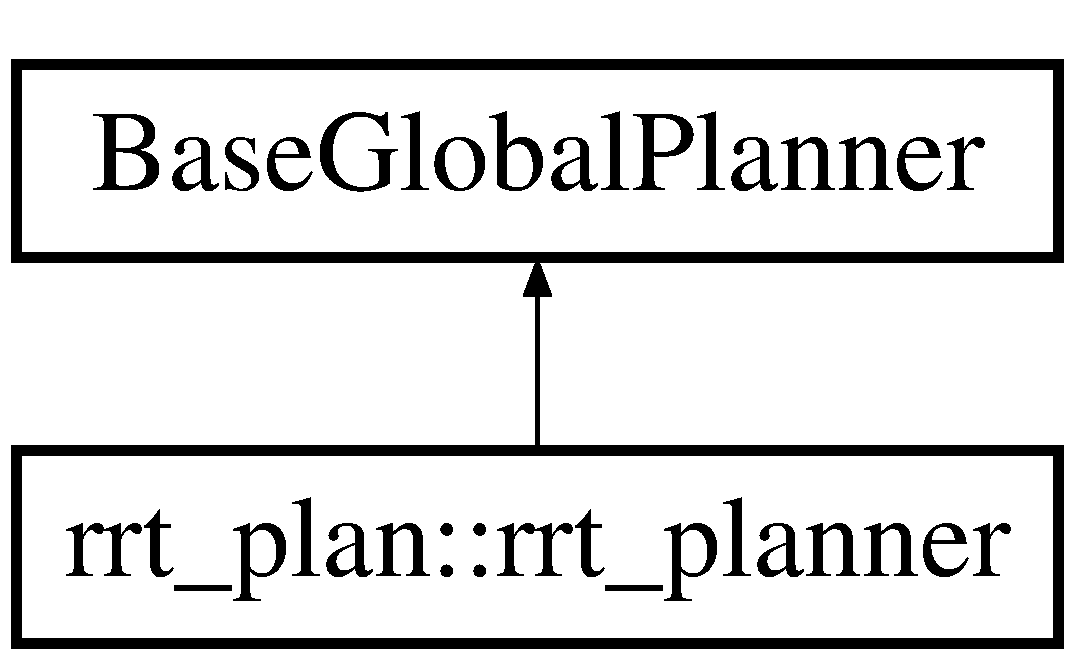
\includegraphics[height=2.000000cm]{classrrt__plan_1_1rrt__planner}
\end{center}
\end{figure}
\subsection*{Public 成员函数}
\begin{DoxyCompactItemize}
\item 
\hyperlink{classrrt__plan_1_1rrt__planner_a188d2961064c51462f133f656b5595ce}{rrt\-\_\-planner} (ros\-::\-Node\-Handle \&)
\item 
\hyperlink{classrrt__plan_1_1rrt__planner_aff0490fe901b891f586fae31433f72f0}{rrt\-\_\-planner} ()
\item 
\hyperlink{classrrt__plan_1_1rrt__planner_a0c6d148e4c72d2cd780831b7b2e7ad2c}{rrt\-\_\-planner} (std\-::string name, costmap\-\_\-2d\-::\-Costmap2\-D\-R\-O\-S $\ast$costmap\-\_\-ros)
\item 
void \hyperlink{classrrt__plan_1_1rrt__planner_aec216e5abd94aa73b71a4db4a3e89c9d}{initialize} (std\-::string name, costmap\-\_\-2d\-::\-Costmap2\-D\-R\-O\-S $\ast$costmap\-\_\-ros)
\item 
bool \hyperlink{classrrt__plan_1_1rrt__planner_a211f1d665d81c1a340d06cdc327fadf4}{make\-Plan} (const geometry\-\_\-msgs\-::\-Pose\-Stamped \&start, const geometry\-\_\-msgs\-::\-Pose\-Stamped \&goal, std\-::vector$<$ geometry\-\_\-msgs\-::\-Pose\-Stamped $>$ \&plan)
\item 
bool \hyperlink{classrrt__plan_1_1rrt__planner_a07347499c296c693631f24dfb1cb4196}{is\-Cell\-Inside\-Map} (float x, float y)
\item 
void \hyperlink{classrrt__plan_1_1rrt__planner_a7cbacb0aead733fc6cfde463c6ea2812}{map\-To\-World} (double mx, double my, double \&wx, double \&wy)
\item 
bool \hyperlink{classrrt__plan_1_1rrt__planner_aa43a4ec62844e679d9e0aefcbfa5f286}{is\-Start\-And\-Goal\-Cells\-Valid} (int start\-Cell, int goal\-Cell)
\item 
bool \hyperlink{classrrt__plan_1_1rrt__planner_a7c923acf8ea571bf84a2ede5a0457491}{is\-Free} (int Cell\-I\-D)
\item 
bool \hyperlink{classrrt__plan_1_1rrt__planner_ac6b3b3e1aa57e2dd76874064f289f370}{is\-Free} (int i, int j)
\item 
vector$<$ int $>$ \hyperlink{classrrt__plan_1_1rrt__planner_a0a4d334b13d1946044f041ae1ddc1a41}{find\-Free\-Neighbor\-Cell} (int Cell\-I\-D)
\item 
vector$<$ int $>$ \hyperlink{classrrt__plan_1_1rrt__planner_a23e32ef1c189f5035a751047f84e052a}{find\-Cell\-Path} (\hyperlink{classRRT}{R\-R\-T} \&\hyperlink{rrt__planner_8cpp_a51725e16375c08b52f82eb2faa5a921c}{my\-R\-R\-T}, int start\-Cell, int goal\-Cell, vector$<$ vector$<$ float $>$ $>$ grid\-Val)
\item 
void \hyperlink{classrrt__plan_1_1rrt__planner_aac5e9f72b4c55ce4aada8d80eed92a9e}{convert\-To\-Plan} (vector$<$ int $>$ best\-Path, std\-::vector$<$ geometry\-\_\-msgs\-::\-Pose\-Stamped $>$ \&plan, geometry\-\_\-msgs\-::\-Pose\-Stamped goal, int goal\-Cell)
\item 
void \hyperlink{classrrt__plan_1_1rrt__planner_ac2fe5313cbc77dffddfcfe1f6605d53e}{publish\-Plan} (const std\-::vector$<$ geometry\-\_\-msgs\-::\-Pose\-Stamped $>$ \&path)
\item 
void \hyperlink{classrrt__plan_1_1rrt__planner_a3071190151c4463f2e39f29c02c1f55d}{publish\-Plan2} (const std\-::vector$<$ geometry\-\_\-msgs\-::\-Pose\-Stamped $>$ \&path)
\item 
void \hyperlink{classrrt__plan_1_1rrt__planner_aff6d98168c072b176287fc9c444349c6}{get\-Grid\-Val} (vector$<$ vector$<$ float $>$ $>$ \&grid\-Val, int start\-Row\-I\-D, int start\-Col\-I\-D, int goal\-Row\-I\-D, int goal\-Col\-I\-D)
\item 
std\-::vector\\*
$<$ geometry\-\_\-msgs\-::\-Pose\-Stamped $>$ \hyperlink{classrrt__plan_1_1rrt__planner_aac168be892772fe17a1d841d87c2249c}{middleoptimization\-Layer} (std\-::vector$<$ geometry\-\_\-msgs\-::\-Pose\-Stamped $>$ temp\-\_\-transformed\-\_\-plan)
\item 
void \hyperlink{classrrt__plan_1_1rrt__planner_a980538776b19bd9610458e45991cdf0b}{get\-Idx} (int \&x, int \&y)
\item 
void \hyperlink{classrrt__plan_1_1rrt__planner_a8f1fde39d2f3b01d7b2d11dc9482e1dc}{get\-Corrdinate} (float \&x, float \&y)
\item 
int \hyperlink{classrrt__plan_1_1rrt__planner_a7df38e380fe80d69be29d1cea2879c59}{get\-Cell\-Index} (int i, int j)
\item 
int \hyperlink{classrrt__plan_1_1rrt__planner_aa3c07d6b2b6bed62e4b60d3898fc80cf}{get\-Cell\-Row\-I\-D} (int index)
\item 
int \hyperlink{classrrt__plan_1_1rrt__planner_a758810b2f257fe0778ed3eb1e970d99c}{get\-Cell\-Col\-I\-D} (int index)
\item 
int \hyperlink{classrrt__plan_1_1rrt__planner_a2647265d06a792b983b372af52cf5677}{convert\-To\-Cell\-Index} (float x, float y)
\item 
void \hyperlink{classrrt__plan_1_1rrt__planner_ad21e1c308a79678ca6265907bf6caa84}{convert\-To\-Coordinate} (int index, float \&x, float \&y)
\item 
bool \hyperlink{classrrt__plan_1_1rrt__planner_a2b6ded4f6e7719510d94371400f097d7}{check\-If\-On\-Obstacles} (\hyperlink{structRRT_1_1rrtNode}{R\-R\-T\-::rrt\-Node} \&temp\-Node)
\item 
void \hyperlink{classrrt__plan_1_1rrt__planner_aaaab60d718aa349ef2df8dcf0402f207}{generate\-Temp\-Point} (\hyperlink{structRRT_1_1rrtNode}{R\-R\-T\-::rrt\-Node} \&temp\-Node, int \hyperlink{classrrt__plan_1_1rrt__planner_ac74fe436b5e1fa30bda1fbe821369aa2}{width}, int \hyperlink{classrrt__plan_1_1rrt__planner_a3549de56a50bff6494514878b64584df}{height})
\item 
void \hyperlink{classrrt__plan_1_1rrt__planner_ac34f8c3a590fb6f3ba04c99500a8abae}{generate\-Rand\-Nodes} (\hyperlink{classRRT}{R\-R\-T} \&\hyperlink{rrt__planner_8cpp_a51725e16375c08b52f82eb2faa5a921c}{my\-R\-R\-T}, vector$<$ \hyperlink{structRRT_1_1rrtNode}{R\-R\-T\-::rrt\-Node} $>$ \&rand\-Nodes, int \hyperlink{classrrt__plan_1_1rrt__planner_ac74fe436b5e1fa30bda1fbe821369aa2}{width}, int \hyperlink{classrrt__plan_1_1rrt__planner_a3549de56a50bff6494514878b64584df}{height})
\item 
double \hyperlink{classrrt__plan_1_1rrt__planner_a7746337004ecc5a7bdad176b5033b5bc}{get\-Rotate\-Angle} (double x1, double y1, double x2, double y2)
\item 
bool \hyperlink{classrrt__plan_1_1rrt__planner_a22cb05cb13d3027310f3fcc2b394dda6}{add\-New\-Nodeto\-R\-R\-T} (\hyperlink{classRRT}{R\-R\-T} \&\hyperlink{rrt__planner_8cpp_a51725e16375c08b52f82eb2faa5a921c}{my\-R\-R\-T}, vector$<$ \hyperlink{structRRT_1_1rrtNode}{R\-R\-T\-::rrt\-Node} $>$ \&rand\-Nodes, float goal\-X, float goal\-Y, int \hyperlink{rrt_8h_aaac2d108c57a5722b9d816baaed80945}{rrt\-Step\-Size}, vector$<$ vector$<$ float $>$ $>$ grid\-Val)
\item 
bool \hyperlink{classrrt__plan_1_1rrt__planner_a50e32f9cd1421d374ea1aab601433b10}{check\-Nodeto\-Goal} (int X, int Y, \hyperlink{structRRT_1_1rrtNode}{R\-R\-T\-::rrt\-Node} \&temp\-Node)
\end{DoxyCompactItemize}
\subsection*{Public 属性}
\begin{DoxyCompactItemize}
\item 
ros\-::\-Node\-Handle \hyperlink{classrrt__plan_1_1rrt__planner_a9547688a6e31166034dc562a0b4608b6}{R\-O\-S\-Node\-Handle}
\item 
float \hyperlink{classrrt__plan_1_1rrt__planner_a92ba133c58a9ad0de8f425e856953ac1}{origin\-X}
\item 
float \hyperlink{classrrt__plan_1_1rrt__planner_a5cfa182b92acb4e370ba19a213a0c22a}{origin\-Y}
\item 
float \hyperlink{classrrt__plan_1_1rrt__planner_ad23ca65f53176297ae7e9f40c7edeb69}{resolution}
\item 
costmap\-\_\-2d\-::\-Costmap2\-D\-R\-O\-S $\ast$ \hyperlink{classrrt__plan_1_1rrt__planner_a3dcf8908136ace532176511eb1861528}{costmap\-\_\-ros\-\_\-}
\item 
double \hyperlink{classrrt__plan_1_1rrt__planner_a25be58fd52b495ade819f8d5785beeae}{step\-\_\-size\-\_\-}
\item 
double \hyperlink{classrrt__plan_1_1rrt__planner_aae70d5e90c66f442c8822b573645e346}{min\-\_\-dist\-\_\-from\-\_\-robot\-\_\-}
\item 
costmap\-\_\-2d\-::\-Costmap2\-D $\ast$ \hyperlink{classrrt__plan_1_1rrt__planner_ad6f48786945a4a394c95de25cd4c77d2}{costmap\-\_\-}
\item 
bool \hyperlink{classrrt__plan_1_1rrt__planner_ac1cd8655573adac056ae922a92337b8d}{initialized\-\_\-}
\item 
int \hyperlink{classrrt__plan_1_1rrt__planner_ac74fe436b5e1fa30bda1fbe821369aa2}{width}
\item 
int \hyperlink{classrrt__plan_1_1rrt__planner_a3549de56a50bff6494514878b64584df}{height}
\item 
ros\-::\-Publisher \hyperlink{classrrt__plan_1_1rrt__planner_a6beed3a62613c7e24813416185d12929}{plan\-\_\-pub\-\_\-}
\item 
ros\-::\-Publisher \hyperlink{classrrt__plan_1_1rrt__planner_a142a2d4c28bcaa2798493accf32690ee}{plan\-\_\-pub\-\_\-2}
\end{DoxyCompactItemize}


\subsection{详细描述}


在文件 inspire\-\_\-rrt\-\_\-planner.\-h 第 76 行定义.



\subsection{构造及析构函数说明}
\hypertarget{classrrt__plan_1_1rrt__planner_a188d2961064c51462f133f656b5595ce}{\index{rrt\-\_\-plan\-::rrt\-\_\-planner@{rrt\-\_\-plan\-::rrt\-\_\-planner}!rrt\-\_\-planner@{rrt\-\_\-planner}}
\index{rrt\-\_\-planner@{rrt\-\_\-planner}!rrt_plan::rrt_planner@{rrt\-\_\-plan\-::rrt\-\_\-planner}}
\subsubsection[{rrt\-\_\-planner}]{\setlength{\rightskip}{0pt plus 5cm}rrt\-\_\-plan\-::rrt\-\_\-planner\-::rrt\-\_\-planner (
\begin{DoxyParamCaption}
\item[{ros\-::\-Node\-Handle \&}]{nh}
\end{DoxyParamCaption}
)}}\label{classrrt__plan_1_1rrt__planner_a188d2961064c51462f133f656b5595ce}


在文件 rrt\-\_\-planner.\-cpp 第 64 行定义.


\begin{DoxyCode}
65 \{
66     \hyperlink{classrrt__plan_1_1rrt__planner_a9547688a6e31166034dc562a0b4608b6}{ROSNodeHandle} = nh;
67 \}
\end{DoxyCode}
\hypertarget{classrrt__plan_1_1rrt__planner_aff0490fe901b891f586fae31433f72f0}{\index{rrt\-\_\-plan\-::rrt\-\_\-planner@{rrt\-\_\-plan\-::rrt\-\_\-planner}!rrt\-\_\-planner@{rrt\-\_\-planner}}
\index{rrt\-\_\-planner@{rrt\-\_\-planner}!rrt_plan::rrt_planner@{rrt\-\_\-plan\-::rrt\-\_\-planner}}
\subsubsection[{rrt\-\_\-planner}]{\setlength{\rightskip}{0pt plus 5cm}rrt\-\_\-plan\-::rrt\-\_\-planner\-::rrt\-\_\-planner (
\begin{DoxyParamCaption}
{}
\end{DoxyParamCaption}
)}}\label{classrrt__plan_1_1rrt__planner_aff0490fe901b891f586fae31433f72f0}


在文件 rrt\-\_\-planner.\-cpp 第 60 行定义.


\begin{DoxyCode}
60                         :\hyperlink{classrrt__plan_1_1rrt__planner_ac1cd8655573adac056ae922a92337b8d}{initialized\_}(\textcolor{keyword}{false})
61 \{
62 
63 \}
\end{DoxyCode}
\hypertarget{classrrt__plan_1_1rrt__planner_a0c6d148e4c72d2cd780831b7b2e7ad2c}{\index{rrt\-\_\-plan\-::rrt\-\_\-planner@{rrt\-\_\-plan\-::rrt\-\_\-planner}!rrt\-\_\-planner@{rrt\-\_\-planner}}
\index{rrt\-\_\-planner@{rrt\-\_\-planner}!rrt_plan::rrt_planner@{rrt\-\_\-plan\-::rrt\-\_\-planner}}
\subsubsection[{rrt\-\_\-planner}]{\setlength{\rightskip}{0pt plus 5cm}rrt\-\_\-plan\-::rrt\-\_\-planner\-::rrt\-\_\-planner (
\begin{DoxyParamCaption}
\item[{std\-::string}]{name, }
\item[{costmap\-\_\-2d\-::\-Costmap2\-D\-R\-O\-S $\ast$}]{costmap\-\_\-ros}
\end{DoxyParamCaption}
)}}\label{classrrt__plan_1_1rrt__planner_a0c6d148e4c72d2cd780831b7b2e7ad2c}


在文件 rrt\-\_\-planner.\-cpp 第 69 行定义.


\begin{DoxyCode}
70 \{
71     \hyperlink{classrrt__plan_1_1rrt__planner_aec216e5abd94aa73b71a4db4a3e89c9d}{initialize}(name, costmap\_ros);
72 \}
\end{DoxyCode}


\subsection{成员函数说明}
\hypertarget{classrrt__plan_1_1rrt__planner_a22cb05cb13d3027310f3fcc2b394dda6}{\index{rrt\-\_\-plan\-::rrt\-\_\-planner@{rrt\-\_\-plan\-::rrt\-\_\-planner}!add\-New\-Nodeto\-R\-R\-T@{add\-New\-Nodeto\-R\-R\-T}}
\index{add\-New\-Nodeto\-R\-R\-T@{add\-New\-Nodeto\-R\-R\-T}!rrt_plan::rrt_planner@{rrt\-\_\-plan\-::rrt\-\_\-planner}}
\subsubsection[{add\-New\-Nodeto\-R\-R\-T}]{\setlength{\rightskip}{0pt plus 5cm}bool rrt\-\_\-plan\-::rrt\-\_\-planner\-::add\-New\-Nodeto\-R\-R\-T (
\begin{DoxyParamCaption}
\item[{{\bf R\-R\-T} \&}]{my\-R\-R\-T, }
\item[{vector$<$ {\bf R\-R\-T\-::rrt\-Node} $>$ \&}]{rand\-Nodes, }
\item[{float}]{goal\-X, }
\item[{float}]{goal\-Y, }
\item[{int}]{rrt\-Step\-Size, }
\item[{vector$<$ vector$<$ float $>$ $>$}]{grid\-Val}
\end{DoxyParamCaption}
)\hspace{0.3cm}{\ttfamily [inline]}}}\label{classrrt__plan_1_1rrt__planner_a22cb05cb13d3027310f3fcc2b394dda6}


在文件 inspire\-\_\-rrt\-\_\-planner.\-h 第 235 行定义.


\begin{DoxyCode}
236     \{
237         vector<RRT::rrtNode> nearestNodes;  \textcolor{comment}{//nearest结点数组}
238         vector<RRT::rrtNode> tempNodes;  \textcolor{comment}{//临时结点数组}
239         \hyperlink{structRRT_1_1rrtNode}{RRT::rrtNode} loopNode;
240 
241         \textcolor{keywordflow}{for}(\textcolor{keywordtype}{int} i=0; i<\hyperlink{rrt_8h_a962f9277eb583fb40d04a820752a9191}{randNodeNum}; i++)
242         \{
243             \textcolor{keywordtype}{int} tempNearestNodeID = myRRT.\hyperlink{classRRT_af35d650011a6b834fc1b2d75b879817c}{getNearestNodeID}(randNodes[i].posX,randNodes[i].
      posY);
244             \hyperlink{structRRT_1_1rrtNode}{RRT::rrtNode} tempNearestNode=myRRT.\hyperlink{classRRT_afde36442771a9552bb97572098396c2b}{getNode}(tempNearestNodeID);
245             nearestNodes.push\_back(tempNearestNode);
246         \}
247 
248         \textcolor{keywordflow}{for}(\textcolor{keywordtype}{int} i=0; i<\hyperlink{rrt_8h_a962f9277eb583fb40d04a820752a9191}{randNodeNum}; i++)
249         \{
250             \textcolor{keywordtype}{double} theta = atan2(randNodes[i].posY - nearestNodes[i].posY, randNodes[i].posX - nearestNodes
      [i].posX);\textcolor{comment}{//两个点形成的斜率}
251             loopNode.\hyperlink{structRRT_1_1rrtNode_a4c2096fa1d719cf2aa49cf21916a5a4b}{posX} = (int)(nearestNodes[i].posX + (\hyperlink{rrt_8h_aaac2d108c57a5722b9d816baaed80945}{rrtStepSize} * cos(theta)));
252             loopNode.\hyperlink{structRRT_1_1rrtNode_a219cf78a0f5689bc84744df52c37e84d}{posY} = (int)(nearestNodes[i].posY + (\hyperlink{rrt_8h_aaac2d108c57a5722b9d816baaed80945}{rrtStepSize} * sin(theta)));
253             loopNode.\hyperlink{structRRT_1_1rrtNode_a9f5b9bfca61e25fe7f80d361ed7996ff}{parentID}=nearestNodes[i].nodeID;  \textcolor{comment}{//temp结点的父结点是它的nearest结点}
254 
255             tempNodes.push\_back(loopNode);
256         \}
257 
258         vector<float> evaluateCost;  \textcolor{comment}{//启发函数估价}
259 
260         \textcolor{keywordflow}{for}(\textcolor{keywordtype}{int} i=0; i<tempNodes.size(); i++)
261         \{
262             \textcolor{keywordtype}{int} tempIndex=i;
263             \hyperlink{structRRT_1_1rrtNode}{RRT::rrtNode} tempNode=tempNodes[i];
264 
265             \textcolor{keywordflow}{if}(\hyperlink{classrrt__plan_1_1rrt__planner_a2b6ded4f6e7719510d94371400f097d7}{checkIfOnObstacles}(tempNode))\textcolor{comment}{//先检查temp结点,不在障碍物上}
266             \{
267                 \textcolor{comment}{//float costG=nearestNodes[i].depth*rrtStepSize;}
268                 \textcolor{keywordtype}{float} costH=gridVal[tempNode.\hyperlink{structRRT_1_1rrtNode_a4c2096fa1d719cf2aa49cf21916a5a4b}{posX}/\hyperlink{rrt_8h_afb8b6147953aaf9e7089f5f157d5b020}{mapReduceSize}][tempNode.
      \hyperlink{structRRT_1_1rrtNode_a219cf78a0f5689bc84744df52c37e84d}{posY}/\hyperlink{rrt_8h_afb8b6147953aaf9e7089f5f157d5b020}{mapReduceSize}];  \textcolor{comment}{//温度场作为代价值}
269                 evaluateCost.push\_back(costH);
270             \}
271             \textcolor{keywordflow}{else}  \textcolor{comment}{//tempNode结点在障碍物上}
272             \{
273                 evaluateCost.push\_back(\hyperlink{rrt_8h_a8bb5664c6d1d0848c059844294c05988}{infinity});  \textcolor{comment}{//障碍物上代价无穷大}
274             \}
275         \}
276 
277         \textcolor{keywordtype}{int} tempIndex=-1;
278         \textcolor{keywordtype}{float} tempCost=\hyperlink{rrt_8h_a8bb5664c6d1d0848c059844294c05988}{infinity};
279         \textcolor{keywordflow}{for}(\textcolor{keywordtype}{int} i=0; i<evaluateCost.size(); i++)
280         \{
281             \textcolor{keywordflow}{if}(evaluateCost[i]<tempCost)
282             \{
283                 tempIndex=i;
284                 tempCost=evaluateCost[i];
285             \}
286         \}
287 
288         \textcolor{keywordflow}{if}(tempIndex!=-1)
289         \{
290             \hyperlink{structRRT_1_1rrtNode}{RRT::rrtNode} successNode=tempNodes[tempIndex];
291             \hyperlink{structRRT_1_1rrtNode}{RRT::rrtNode} nearestNode=nearestNodes[tempIndex];
292             \textcolor{keywordtype}{float} costN=gridVal[nearestNode.\hyperlink{structRRT_1_1rrtNode_a4c2096fa1d719cf2aa49cf21916a5a4b}{posX}/\hyperlink{rrt_8h_afb8b6147953aaf9e7089f5f157d5b020}{mapReduceSize}][nearestNode.
      \hyperlink{structRRT_1_1rrtNode_a219cf78a0f5689bc84744df52c37e84d}{posY}/\hyperlink{rrt_8h_afb8b6147953aaf9e7089f5f157d5b020}{mapReduceSize}];  \textcolor{comment}{//温度场作为代价值}
293             
294             \textcolor{keywordflow}{if}(evaluateCost[tempIndex]>costN)  \textcolor{comment}{//防止RRT随机树退化}
295                 \textcolor{keywordflow}{return} \textcolor{keyword}{false};
296             
297             \textcolor{keywordtype}{float} tempToParentDistance=\hyperlink{rrt_8h_aaac2d108c57a5722b9d816baaed80945}{rrtStepSize};
298             \textcolor{keywordtype}{bool} regressionFlag=\textcolor{keyword}{true};
299             \textcolor{keywordflow}{for}(\textcolor{keywordtype}{int} i=0; i<myRRT.\hyperlink{classRRT_a05dc852e0b777042e290dcc96bf605bb}{getTreeSize}(); i++)
300             \{
301                 \textcolor{keywordtype}{float} tempDistance=sqrt(pow(myRRT.\hyperlink{classRRT_afde36442771a9552bb97572098396c2b}{getNode}(i).\hyperlink{structRRT_1_1rrtNode_a4c2096fa1d719cf2aa49cf21916a5a4b}{posX} - successNode.
      \hyperlink{structRRT_1_1rrtNode_a4c2096fa1d719cf2aa49cf21916a5a4b}{posX},2) + pow(myRRT.\hyperlink{classRRT_afde36442771a9552bb97572098396c2b}{getNode}(i).\hyperlink{structRRT_1_1rrtNode_a219cf78a0f5689bc84744df52c37e84d}{posY} - successNode.\hyperlink{structRRT_1_1rrtNode_a219cf78a0f5689bc84744df52c37e84d}{posY},2));
302 
303                 \textcolor{keywordflow}{if}(tempToParentDistance-tempDistance>1)
304                 \{
305                     regressionFlag=\textcolor{keyword}{false};
306                     \textcolor{keywordflow}{break};
307                 \}
308             \}
309             
310             \textcolor{keywordflow}{if}(regressionFlag)
311             \{
312                 successNode.\hyperlink{structRRT_1_1rrtNode_aa8adf5b50e1a2a466771ae3af56b1658}{nodeID} = myRRT.\hyperlink{classRRT_a05dc852e0b777042e290dcc96bf605bb}{getTreeSize}();\textcolor{comment}{//设置tempNode的id值,结点个数代表编号}
313                 successNode.\hyperlink{structRRT_1_1rrtNode_ab20e6f5be075c8feed605c935924df30}{depth}=nearestNodes[tempIndex].depth+1;\textcolor{comment}{//当前结点深度等于其父结点深度加1}
314 
315                 myRRT.\hyperlink{classRRT_a5a0591369964c82b95f08c9f868dbd54}{addNewNode}(successNode);
316 
317                 \textcolor{keywordflow}{return} \textcolor{keyword}{true};
318             \}
319         \}
320 
321         \textcolor{keywordflow}{return} \textcolor{keyword}{false};
322     \}
\end{DoxyCode}
\hypertarget{classrrt__plan_1_1rrt__planner_a2b6ded4f6e7719510d94371400f097d7}{\index{rrt\-\_\-plan\-::rrt\-\_\-planner@{rrt\-\_\-plan\-::rrt\-\_\-planner}!check\-If\-On\-Obstacles@{check\-If\-On\-Obstacles}}
\index{check\-If\-On\-Obstacles@{check\-If\-On\-Obstacles}!rrt_plan::rrt_planner@{rrt\-\_\-plan\-::rrt\-\_\-planner}}
\subsubsection[{check\-If\-On\-Obstacles}]{\setlength{\rightskip}{0pt plus 5cm}bool rrt\-\_\-plan\-::rrt\-\_\-planner\-::check\-If\-On\-Obstacles (
\begin{DoxyParamCaption}
\item[{{\bf R\-R\-T\-::rrt\-Node} \&}]{temp\-Node}
\end{DoxyParamCaption}
)}}\label{classrrt__plan_1_1rrt__planner_a2b6ded4f6e7719510d94371400f097d7}


在文件 rrt\-\_\-planner.\-cpp 第 764 行定义.


\begin{DoxyCode}
765 \{
766     \textcolor{keywordflow}{if}((tempNode.\hyperlink{structRRT_1_1rrtNode_a4c2096fa1d719cf2aa49cf21916a5a4b}{posX}<\hyperlink{classrrt__plan_1_1rrt__planner_ac74fe436b5e1fa30bda1fbe821369aa2}{width})&&(tempNode.\hyperlink{structRRT_1_1rrtNode_a219cf78a0f5689bc84744df52c37e84d}{posY}<\hyperlink{classrrt__plan_1_1rrt__planner_a3549de56a50bff6494514878b64584df}{height}))
767     \{
768         \textcolor{keywordflow}{if}(\hyperlink{rrt__planner_8cpp_ab8e6863a3519a503a24344e88545eb3d}{OGM}[\hyperlink{classrrt__plan_1_1rrt__planner_a7df38e380fe80d69be29d1cea2879c59}{getCellIndex}(tempNode.\hyperlink{structRRT_1_1rrtNode_a4c2096fa1d719cf2aa49cf21916a5a4b}{posX},tempNode.\hyperlink{structRRT_1_1rrtNode_a219cf78a0f5689bc84744df52c37e84d}{posY})])
769             \textcolor{keywordflow}{return} \textcolor{keyword}{true};
770         \textcolor{keywordflow}{else}
771             \textcolor{keywordflow}{return} \textcolor{keyword}{false};
772     \}
773     \textcolor{keywordflow}{else}
774         \textcolor{keywordflow}{return} \textcolor{keyword}{false};
775 \}
\end{DoxyCode}
\hypertarget{classrrt__plan_1_1rrt__planner_a50e32f9cd1421d374ea1aab601433b10}{\index{rrt\-\_\-plan\-::rrt\-\_\-planner@{rrt\-\_\-plan\-::rrt\-\_\-planner}!check\-Nodeto\-Goal@{check\-Nodeto\-Goal}}
\index{check\-Nodeto\-Goal@{check\-Nodeto\-Goal}!rrt_plan::rrt_planner@{rrt\-\_\-plan\-::rrt\-\_\-planner}}
\subsubsection[{check\-Nodeto\-Goal}]{\setlength{\rightskip}{0pt plus 5cm}bool rrt\-\_\-plan\-::rrt\-\_\-planner\-::check\-Nodeto\-Goal (
\begin{DoxyParamCaption}
\item[{int}]{X, }
\item[{int}]{Y, }
\item[{{\bf R\-R\-T\-::rrt\-Node} \&}]{temp\-Node}
\end{DoxyParamCaption}
)\hspace{0.3cm}{\ttfamily [inline]}}}\label{classrrt__plan_1_1rrt__planner_a50e32f9cd1421d374ea1aab601433b10}


在文件 inspire\-\_\-rrt\-\_\-planner.\-h 第 324 行定义.


\begin{DoxyCode}
325     \{
326         \textcolor{keywordtype}{double} distance = sqrt(pow(X-tempNode.\hyperlink{structRRT_1_1rrtNode_a4c2096fa1d719cf2aa49cf21916a5a4b}{posX},2)+pow(Y-tempNode.\hyperlink{structRRT_1_1rrtNode_a219cf78a0f5689bc84744df52c37e84d}{posY},2));
327         \textcolor{keywordflow}{if}(distance < \hyperlink{rrt_8h_aaac2d108c57a5722b9d816baaed80945}{rrtStepSize})  \textcolor{comment}{//goal与nearest之间距离小于rrtStepSize时即认为到达目标点}
328         \{
329             \textcolor{keywordflow}{return} \textcolor{keyword}{true};
330         \}
331         \textcolor{keywordflow}{return} \textcolor{keyword}{false};
332     \}
\end{DoxyCode}
\hypertarget{classrrt__plan_1_1rrt__planner_a2647265d06a792b983b372af52cf5677}{\index{rrt\-\_\-plan\-::rrt\-\_\-planner@{rrt\-\_\-plan\-::rrt\-\_\-planner}!convert\-To\-Cell\-Index@{convert\-To\-Cell\-Index}}
\index{convert\-To\-Cell\-Index@{convert\-To\-Cell\-Index}!rrt_plan::rrt_planner@{rrt\-\_\-plan\-::rrt\-\_\-planner}}
\subsubsection[{convert\-To\-Cell\-Index}]{\setlength{\rightskip}{0pt plus 5cm}int rrt\-\_\-plan\-::rrt\-\_\-planner\-::convert\-To\-Cell\-Index (
\begin{DoxyParamCaption}
\item[{float}]{x, }
\item[{float}]{y}
\end{DoxyParamCaption}
)\hspace{0.3cm}{\ttfamily [inline]}}}\label{classrrt__plan_1_1rrt__planner_a2647265d06a792b983b372af52cf5677}


在文件 inspire\-\_\-rrt\-\_\-planner.\-h 第 135 行定义.


\begin{DoxyCode}
136     \{
137         \textcolor{keywordtype}{int} cellIndex;
138 
139         \textcolor{keywordtype}{float} newX = x / \hyperlink{classrrt__plan_1_1rrt__planner_ad23ca65f53176297ae7e9f40c7edeb69}{resolution};
140         \textcolor{keywordtype}{float} newY = y / \hyperlink{classrrt__plan_1_1rrt__planner_ad23ca65f53176297ae7e9f40c7edeb69}{resolution};
141 
142         cellIndex = \hyperlink{classrrt__plan_1_1rrt__planner_a7df38e380fe80d69be29d1cea2879c59}{getCellIndex}(newY, newX);
143 
144         \textcolor{keywordflow}{return} cellIndex;
145     \}
\end{DoxyCode}
\hypertarget{classrrt__plan_1_1rrt__planner_ad21e1c308a79678ca6265907bf6caa84}{\index{rrt\-\_\-plan\-::rrt\-\_\-planner@{rrt\-\_\-plan\-::rrt\-\_\-planner}!convert\-To\-Coordinate@{convert\-To\-Coordinate}}
\index{convert\-To\-Coordinate@{convert\-To\-Coordinate}!rrt_plan::rrt_planner@{rrt\-\_\-plan\-::rrt\-\_\-planner}}
\subsubsection[{convert\-To\-Coordinate}]{\setlength{\rightskip}{0pt plus 5cm}void rrt\-\_\-plan\-::rrt\-\_\-planner\-::convert\-To\-Coordinate (
\begin{DoxyParamCaption}
\item[{int}]{index, }
\item[{float \&}]{x, }
\item[{float \&}]{y}
\end{DoxyParamCaption}
)\hspace{0.3cm}{\ttfamily [inline]}}}\label{classrrt__plan_1_1rrt__planner_ad21e1c308a79678ca6265907bf6caa84}


在文件 inspire\-\_\-rrt\-\_\-planner.\-h 第 148 行定义.


\begin{DoxyCode}
149     \{
150         x = \hyperlink{classrrt__plan_1_1rrt__planner_a758810b2f257fe0778ed3eb1e970d99c}{getCellColID}(index) * \hyperlink{classrrt__plan_1_1rrt__planner_ad23ca65f53176297ae7e9f40c7edeb69}{resolution};
151 
152         y = \hyperlink{classrrt__plan_1_1rrt__planner_aa3c07d6b2b6bed62e4b60d3898fc80cf}{getCellRowID}(index) * \hyperlink{classrrt__plan_1_1rrt__planner_ad23ca65f53176297ae7e9f40c7edeb69}{resolution};
153 
154         x = x + \hyperlink{classrrt__plan_1_1rrt__planner_a92ba133c58a9ad0de8f425e856953ac1}{originX};
155         y = y + \hyperlink{classrrt__plan_1_1rrt__planner_a5cfa182b92acb4e370ba19a213a0c22a}{originY};
156     \}
\end{DoxyCode}
\hypertarget{classrrt__plan_1_1rrt__planner_aac5e9f72b4c55ce4aada8d80eed92a9e}{\index{rrt\-\_\-plan\-::rrt\-\_\-planner@{rrt\-\_\-plan\-::rrt\-\_\-planner}!convert\-To\-Plan@{convert\-To\-Plan}}
\index{convert\-To\-Plan@{convert\-To\-Plan}!rrt_plan::rrt_planner@{rrt\-\_\-plan\-::rrt\-\_\-planner}}
\subsubsection[{convert\-To\-Plan}]{\setlength{\rightskip}{0pt plus 5cm}void rrt\-\_\-plan\-::rrt\-\_\-planner\-::convert\-To\-Plan (
\begin{DoxyParamCaption}
\item[{vector$<$ int $>$}]{best\-Path, }
\item[{std\-::vector$<$ geometry\-\_\-msgs\-::\-Pose\-Stamped $>$ \&}]{plan, }
\item[{geometry\-\_\-msgs\-::\-Pose\-Stamped}]{goal, }
\item[{int}]{goal\-Cell}
\end{DoxyParamCaption}
)}}\label{classrrt__plan_1_1rrt__planner_aac5e9f72b4c55ce4aada8d80eed92a9e}


在文件 rrt\-\_\-planner.\-cpp 第 692 行定义.


\begin{DoxyCode}
693 \{
694     \textcolor{comment}{// convert the path}
695     \textcolor{keywordflow}{for} (\textcolor{keywordtype}{int} i = 0; i < rrtPath.size(); i++)
696     \{
697 
698         \textcolor{keywordtype}{float} x = 0.0;
699         \textcolor{keywordtype}{float} y = 0.0;
700 
701         \textcolor{keywordtype}{int} tempNodeId=rrtPath[i];
702         \textcolor{keywordtype}{int} cellIndex=\hyperlink{classrrt__plan_1_1rrt__planner_a7df38e380fe80d69be29d1cea2879c59}{getCellIndex}(\hyperlink{rrt__planner_8cpp_a51725e16375c08b52f82eb2faa5a921c}{myRRT}.\hyperlink{classRRT_a54760030f6b61b258b6eec4472ced906}{getPosX}(tempNodeId),
      \hyperlink{rrt__planner_8cpp_a51725e16375c08b52f82eb2faa5a921c}{myRRT}.\hyperlink{classRRT_a499a6d42d47b76c306a80573cba0a555}{getPosY}(tempNodeId));
703 
704 
705         \hyperlink{classrrt__plan_1_1rrt__planner_ad21e1c308a79678ca6265907bf6caa84}{convertToCoordinate}(cellIndex, x, y);
706 
707         \textcolor{comment}{//cout<<"--cell"<<index<<": x="<<x<<",y="<<y<<endl;}
708         \textcolor{comment}{//rrtlog<<"--cell"<<index<<": x="<<x<<",y="<<y<<endl;}
709 
710         geometry\_msgs::PoseStamped pose = goal;
711 
712 
713         pose.pose.position.x = x;
714         pose.pose.position.y = y;
715         pose.pose.position.z = 0.0;
716 
717         pose.pose.orientation.x = 0.0;
718         pose.pose.orientation.y = 0.0;
719         pose.pose.orientation.z = 0.0;
720         pose.pose.orientation.w = 1.0;
721 
722         plan.push\_back(pose);
723     \}
724 
725 
726     \textcolor{comment}{//处理最后一个结点,即是目标点goal}
727     \textcolor{keywordtype}{float} final\_x = 0.0;
728     \textcolor{keywordtype}{float} final\_y = 0.0;
729     \textcolor{keywordtype}{int} final\_index = goalCell;
730     \hyperlink{classrrt__plan_1_1rrt__planner_ad21e1c308a79678ca6265907bf6caa84}{convertToCoordinate}(final\_index, final\_x, final\_y);
731     \textcolor{comment}{//cout<<"--cell"<<final\_index<<": final\_x="<<final\_x<<",final\_y="<<final\_y<<endl;}
732     \textcolor{comment}{//rrtlog<<"--cell"<<final\_index<<": final\_x="<<final\_x<<",final\_y="<<final\_y<<endl;}
733 
734     geometry\_msgs::PoseStamped final\_pose = goal;
735     final\_pose.pose.position.x = final\_x;
736     final\_pose.pose.position.y = final\_y;
737     final\_pose.pose.position.z = 0.0;
738     final\_pose.pose.orientation.x = 0.0;
739     final\_pose.pose.orientation.y = 0.0;
740     final\_pose.pose.orientation.z = 0.0;
741     final\_pose.pose.orientation.w = 1.0;
742     plan.push\_back(final\_pose);  \textcolor{comment}{//最后一个结点,即是目标点}
743 
744 
745     \textcolor{comment}{/*}
746 \textcolor{comment}{    float path\_length = 0.0;}
747 \textcolor{comment}{    std::vector<geometry\_msgs::PoseStamped>::iterator it = plan.begin();}
748 \textcolor{comment}{}
749 \textcolor{comment}{    geometry\_msgs::PoseStamped last\_pose;}
750 \textcolor{comment}{    last\_pose = *it;}
751 \textcolor{comment}{    it++;}
752 \textcolor{comment}{    for (; it!=plan.end(); ++it) \{}
753 \textcolor{comment}{        path\_length += hypot(  (*it).pose.position.x - last\_pose.pose.position.x,}
754 \textcolor{comment}{                  (*it).pose.position.y - last\_pose.pose.position.y );}
755 \textcolor{comment}{        last\_pose = *it;}
756 \textcolor{comment}{    \}}
757 \textcolor{comment}{    *}
758 \textcolor{comment}{    */}
759 
760     \textcolor{comment}{//cout <<"The global path length: "<< path\_length<< " meters"<<endl;}
761     \textcolor{comment}{//rrtlog<<"The global path length: "<< path\_length<< " meters"<<endl;}
762 \}
\end{DoxyCode}
\hypertarget{classrrt__plan_1_1rrt__planner_a23e32ef1c189f5035a751047f84e052a}{\index{rrt\-\_\-plan\-::rrt\-\_\-planner@{rrt\-\_\-plan\-::rrt\-\_\-planner}!find\-Cell\-Path@{find\-Cell\-Path}}
\index{find\-Cell\-Path@{find\-Cell\-Path}!rrt_plan::rrt_planner@{rrt\-\_\-plan\-::rrt\-\_\-planner}}
\subsubsection[{find\-Cell\-Path}]{\setlength{\rightskip}{0pt plus 5cm}vector$<$ int $>$ rrt\-\_\-plan\-::rrt\-\_\-planner\-::find\-Cell\-Path (
\begin{DoxyParamCaption}
\item[{{\bf R\-R\-T} \&}]{my\-R\-R\-T, }
\item[{int}]{start\-Cell, }
\item[{int}]{goal\-Cell, }
\item[{vector$<$ vector$<$ float $>$ $>$}]{grid\-Val}
\end{DoxyParamCaption}
)}}\label{classrrt__plan_1_1rrt__planner_a23e32ef1c189f5035a751047f84e052a}


在文件 rrt\-\_\-planner.\-cpp 第 651 行定义.


\begin{DoxyCode}
652 \{
653     vector<int>  rrtPath;
654 
655     vector<RRT::rrtNode> randNodes;
656 
657     \textcolor{keywordtype}{bool} addNodeResult = \textcolor{keyword}{false}, nodeToGoal = \textcolor{keyword}{false};
658 
659     \textcolor{keywordflow}{while}(1)
660     \{
661         randNodes.clear();
662         \textcolor{comment}{//generateTempPoint(tempNode,width, height);  //一次产生一个随机结点}
663         \hyperlink{classrrt__plan_1_1rrt__planner_ac34f8c3a590fb6f3ba04c99500a8abae}{generateRandNodes}( myRRT,randNodes,\hyperlink{classrrt__plan_1_1rrt__planner_ac74fe436b5e1fa30bda1fbe821369aa2}{width}, \hyperlink{classrrt__plan_1_1rrt__planner_a3549de56a50bff6494514878b64584df}{height});  \textcolor{comment}{//一次产生一个随机结点数组}
664 
665         \textcolor{comment}{//addNodeResult = addNewPointtoRRT(myRRT,tempNode,rrtStepSize);  //经典RRT方法添加新结点}
666         addNodeResult = \hyperlink{classrrt__plan_1_1rrt__planner_a22cb05cb13d3027310f3fcc2b394dda6}{addNewNodetoRRT}(myRRT,randNodes,
      \hyperlink{classrrt__plan_1_1rrt__planner_aa3c07d6b2b6bed62e4b60d3898fc80cf}{getCellRowID}(goalCell), \hyperlink{classrrt__plan_1_1rrt__planner_a758810b2f257fe0778ed3eb1e970d99c}{getCellColID}(goalCell),
      \hyperlink{rrt_8h_aaac2d108c57a5722b9d816baaed80945}{rrtStepSize},gridVal); \textcolor{comment}{//启发函数优化RRT方法}
667 
668         \textcolor{keywordflow}{if}(addNodeResult)
669         \{
670             \textcolor{comment}{//nodeToGoal = checkNodetoGoal(getCellRowID(goalCell),
       getCellColID(goalCell),tempNode);//经典RRT方法添加新结点}
671 
672             \hyperlink{structRRT_1_1rrtNode}{RRT::rrtNode} lastNode=myRRT.\hyperlink{classRRT_afde36442771a9552bb97572098396c2b}{getNode}(myRRT.
      \hyperlink{classRRT_a05dc852e0b777042e290dcc96bf605bb}{getTreeSize}()-1);
673             nodeToGoal = \hyperlink{classrrt__plan_1_1rrt__planner_a50e32f9cd1421d374ea1aab601433b10}{checkNodetoGoal}(\hyperlink{classrrt__plan_1_1rrt__planner_aa3c07d6b2b6bed62e4b60d3898fc80cf}{getCellRowID}(goalCell), 
      \hyperlink{classrrt__plan_1_1rrt__planner_a758810b2f257fe0778ed3eb1e970d99c}{getCellColID}(goalCell),lastNode);\textcolor{comment}{//启发函数优化RRT方法}
674 
675             \textcolor{keywordflow}{if}(nodeToGoal)
676             \{
677                 \textcolor{comment}{//path = myRRT.getRootToEndPath(tempNode.nodeID);//经典RRT方法得到路径}
678 
679                 rrtPath = myRRT.\hyperlink{classRRT_a487dc3036806a9fb506a718257d8a846}{getRootToEndPath}(myRRT.
      \hyperlink{classRRT_a05dc852e0b777042e290dcc96bf605bb}{getTreeSize}()-1);\textcolor{comment}{//启发函数优化RRT方法得到路径}
680 
681                 \textcolor{keywordflow}{break};
682             \}
683         \}
684     \}
685 
686     cout<<\textcolor{stringliteral}{"RRT nodeSum="}<<myRRT.\hyperlink{classRRT_a05dc852e0b777042e290dcc96bf605bb}{getTreeSize}()<<endl;
687     \hyperlink{rrt__planner_8cpp_ae63d6003ff9416f7c0be6892e5bb899c}{irrtlog}<<\textcolor{stringliteral}{"RRT nodeSum="}<<myRRT.\hyperlink{classRRT_a05dc852e0b777042e290dcc96bf605bb}{getTreeSize}()<<endl;
688 
689     \textcolor{keywordflow}{return} rrtPath;
690 \}
\end{DoxyCode}
\hypertarget{classrrt__plan_1_1rrt__planner_a0a4d334b13d1946044f041ae1ddc1a41}{\index{rrt\-\_\-plan\-::rrt\-\_\-planner@{rrt\-\_\-plan\-::rrt\-\_\-planner}!find\-Free\-Neighbor\-Cell@{find\-Free\-Neighbor\-Cell}}
\index{find\-Free\-Neighbor\-Cell@{find\-Free\-Neighbor\-Cell}!rrt_plan::rrt_planner@{rrt\-\_\-plan\-::rrt\-\_\-planner}}
\subsubsection[{find\-Free\-Neighbor\-Cell}]{\setlength{\rightskip}{0pt plus 5cm}vector$<$ int $>$ rrt\-\_\-plan\-::rrt\-\_\-planner\-::find\-Free\-Neighbor\-Cell (
\begin{DoxyParamCaption}
\item[{int}]{Cell\-I\-D}
\end{DoxyParamCaption}
)}}\label{classrrt__plan_1_1rrt__planner_a0a4d334b13d1946044f041ae1ddc1a41}


在文件 rrt\-\_\-planner.\-cpp 第 809 行定义.


\begin{DoxyCode}
810 \{
811 
812     \textcolor{keywordtype}{int} rowID=\hyperlink{classrrt__plan_1_1rrt__planner_aa3c07d6b2b6bed62e4b60d3898fc80cf}{getCellRowID}(CellID);
813     \textcolor{keywordtype}{int} colID=\hyperlink{classrrt__plan_1_1rrt__planner_a758810b2f257fe0778ed3eb1e970d99c}{getCellColID}(CellID);
814     \textcolor{keywordtype}{int} neighborIndex;
815     vector <int>  freeNeighborCells;
816 
817     \textcolor{keywordflow}{for} (\textcolor{keywordtype}{int} i=-1; i<=1; i++)
818         \textcolor{keywordflow}{for} (\textcolor{keywordtype}{int} j=-1; j<=1; j++)
819         \{
820             \textcolor{comment}{//check whether the index is valid}
821             \textcolor{keywordflow}{if} ((rowID+i>=0)&&(rowID+i<\hyperlink{classrrt__plan_1_1rrt__planner_a3549de56a50bff6494514878b64584df}{height})&&(colID+j>=0)&&(colID+j<
      \hyperlink{classrrt__plan_1_1rrt__planner_ac74fe436b5e1fa30bda1fbe821369aa2}{width})&& (!(i==0 && j==0)))
822             \{
823                 neighborIndex = \hyperlink{classrrt__plan_1_1rrt__planner_a7df38e380fe80d69be29d1cea2879c59}{getCellIndex}(rowID+i,colID+j);
824                 \textcolor{keywordflow}{if}(\hyperlink{classrrt__plan_1_1rrt__planner_a7c923acf8ea571bf84a2ede5a0457491}{isFree}(neighborIndex) )
825                     freeNeighborCells.push\_back(neighborIndex);
826             \}
827         \}
828     \textcolor{keywordflow}{return}  freeNeighborCells;
829 
830 \}
\end{DoxyCode}
\hypertarget{classrrt__plan_1_1rrt__planner_ac34f8c3a590fb6f3ba04c99500a8abae}{\index{rrt\-\_\-plan\-::rrt\-\_\-planner@{rrt\-\_\-plan\-::rrt\-\_\-planner}!generate\-Rand\-Nodes@{generate\-Rand\-Nodes}}
\index{generate\-Rand\-Nodes@{generate\-Rand\-Nodes}!rrt_plan::rrt_planner@{rrt\-\_\-plan\-::rrt\-\_\-planner}}
\subsubsection[{generate\-Rand\-Nodes}]{\setlength{\rightskip}{0pt plus 5cm}void rrt\-\_\-plan\-::rrt\-\_\-planner\-::generate\-Rand\-Nodes (
\begin{DoxyParamCaption}
\item[{{\bf R\-R\-T} \&}]{my\-R\-R\-T, }
\item[{vector$<$ {\bf R\-R\-T\-::rrt\-Node} $>$ \&}]{rand\-Nodes, }
\item[{int}]{width, }
\item[{int}]{height}
\end{DoxyParamCaption}
)\hspace{0.3cm}{\ttfamily [inline]}}}\label{classrrt__plan_1_1rrt__planner_ac34f8c3a590fb6f3ba04c99500a8abae}


在文件 inspire\-\_\-rrt\-\_\-planner.\-h 第 168 行定义.


\begin{DoxyCode}
169     \{
170         \hyperlink{structRRT_1_1rrtNode}{RRT::rrtNode} loopNode;
171 
172         \textcolor{keywordflow}{for}(\textcolor{keywordtype}{int} i=0; i<\hyperlink{rrt_8h_a962f9277eb583fb40d04a820752a9191}{randNodeNum}; i++)
173         \{
174             \textcolor{keywordtype}{int} x = rand() % \hyperlink{classrrt__plan_1_1rrt__planner_ac74fe436b5e1fa30bda1fbe821369aa2}{width} + 1;  \textcolor{comment}{//行}
175             \textcolor{keywordtype}{int} y = rand() % \hyperlink{classrrt__plan_1_1rrt__planner_a3549de56a50bff6494514878b64584df}{height} + 1;  \textcolor{comment}{//列}
176           
177             loopNode.\hyperlink{structRRT_1_1rrtNode_a4c2096fa1d719cf2aa49cf21916a5a4b}{posX} = x;
178             loopNode.\hyperlink{structRRT_1_1rrtNode_a219cf78a0f5689bc84744df52c37e84d}{posY} = y;
179 
180             randNodes.push\_back(loopNode);
181         \}
182 
183     \}
\end{DoxyCode}
\hypertarget{classrrt__plan_1_1rrt__planner_aaaab60d718aa349ef2df8dcf0402f207}{\index{rrt\-\_\-plan\-::rrt\-\_\-planner@{rrt\-\_\-plan\-::rrt\-\_\-planner}!generate\-Temp\-Point@{generate\-Temp\-Point}}
\index{generate\-Temp\-Point@{generate\-Temp\-Point}!rrt_plan::rrt_planner@{rrt\-\_\-plan\-::rrt\-\_\-planner}}
\subsubsection[{generate\-Temp\-Point}]{\setlength{\rightskip}{0pt plus 5cm}void rrt\-\_\-plan\-::rrt\-\_\-planner\-::generate\-Temp\-Point (
\begin{DoxyParamCaption}
\item[{{\bf R\-R\-T\-::rrt\-Node} \&}]{temp\-Node, }
\item[{int}]{width, }
\item[{int}]{height}
\end{DoxyParamCaption}
)\hspace{0.3cm}{\ttfamily [inline]}}}\label{classrrt__plan_1_1rrt__planner_aaaab60d718aa349ef2df8dcf0402f207}


在文件 inspire\-\_\-rrt\-\_\-planner.\-h 第 160 行定义.


\begin{DoxyCode}
161     \{
162         \textcolor{keywordtype}{int} x = rand() % \hyperlink{classrrt__plan_1_1rrt__planner_ac74fe436b5e1fa30bda1fbe821369aa2}{width} + 1;  \textcolor{comment}{//行}
163         \textcolor{keywordtype}{int} y = rand() % \hyperlink{classrrt__plan_1_1rrt__planner_a3549de56a50bff6494514878b64584df}{height} + 1;  \textcolor{comment}{//列}
164         tempNode.\hyperlink{structRRT_1_1rrtNode_a4c2096fa1d719cf2aa49cf21916a5a4b}{posX} = x;
165         tempNode.\hyperlink{structRRT_1_1rrtNode_a219cf78a0f5689bc84744df52c37e84d}{posY} = y;
166     \}
\end{DoxyCode}
\hypertarget{classrrt__plan_1_1rrt__planner_a758810b2f257fe0778ed3eb1e970d99c}{\index{rrt\-\_\-plan\-::rrt\-\_\-planner@{rrt\-\_\-plan\-::rrt\-\_\-planner}!get\-Cell\-Col\-I\-D@{get\-Cell\-Col\-I\-D}}
\index{get\-Cell\-Col\-I\-D@{get\-Cell\-Col\-I\-D}!rrt_plan::rrt_planner@{rrt\-\_\-plan\-::rrt\-\_\-planner}}
\subsubsection[{get\-Cell\-Col\-I\-D}]{\setlength{\rightskip}{0pt plus 5cm}int rrt\-\_\-plan\-::rrt\-\_\-planner\-::get\-Cell\-Col\-I\-D (
\begin{DoxyParamCaption}
\item[{int}]{index}
\end{DoxyParamCaption}
)\hspace{0.3cm}{\ttfamily [inline]}}}\label{classrrt__plan_1_1rrt__planner_a758810b2f257fe0778ed3eb1e970d99c}


在文件 inspire\-\_\-rrt\-\_\-planner.\-h 第 130 行定义.


\begin{DoxyCode}
131     \{
132         \textcolor{keywordflow}{return} index%\hyperlink{classrrt__plan_1_1rrt__planner_ac74fe436b5e1fa30bda1fbe821369aa2}{width};
133     \}
\end{DoxyCode}
\hypertarget{classrrt__plan_1_1rrt__planner_a7df38e380fe80d69be29d1cea2879c59}{\index{rrt\-\_\-plan\-::rrt\-\_\-planner@{rrt\-\_\-plan\-::rrt\-\_\-planner}!get\-Cell\-Index@{get\-Cell\-Index}}
\index{get\-Cell\-Index@{get\-Cell\-Index}!rrt_plan::rrt_planner@{rrt\-\_\-plan\-::rrt\-\_\-planner}}
\subsubsection[{get\-Cell\-Index}]{\setlength{\rightskip}{0pt plus 5cm}int rrt\-\_\-plan\-::rrt\-\_\-planner\-::get\-Cell\-Index (
\begin{DoxyParamCaption}
\item[{int}]{i, }
\item[{int}]{j}
\end{DoxyParamCaption}
)\hspace{0.3cm}{\ttfamily [inline]}}}\label{classrrt__plan_1_1rrt__planner_a7df38e380fe80d69be29d1cea2879c59}


在文件 inspire\-\_\-rrt\-\_\-planner.\-h 第 120 行定义.


\begin{DoxyCode}
121     \{
122         \textcolor{keywordflow}{return} (i*\hyperlink{classrrt__plan_1_1rrt__planner_ac74fe436b5e1fa30bda1fbe821369aa2}{width})+j;
123     \}
\end{DoxyCode}
\hypertarget{classrrt__plan_1_1rrt__planner_aa3c07d6b2b6bed62e4b60d3898fc80cf}{\index{rrt\-\_\-plan\-::rrt\-\_\-planner@{rrt\-\_\-plan\-::rrt\-\_\-planner}!get\-Cell\-Row\-I\-D@{get\-Cell\-Row\-I\-D}}
\index{get\-Cell\-Row\-I\-D@{get\-Cell\-Row\-I\-D}!rrt_plan::rrt_planner@{rrt\-\_\-plan\-::rrt\-\_\-planner}}
\subsubsection[{get\-Cell\-Row\-I\-D}]{\setlength{\rightskip}{0pt plus 5cm}int rrt\-\_\-plan\-::rrt\-\_\-planner\-::get\-Cell\-Row\-I\-D (
\begin{DoxyParamCaption}
\item[{int}]{index}
\end{DoxyParamCaption}
)\hspace{0.3cm}{\ttfamily [inline]}}}\label{classrrt__plan_1_1rrt__planner_aa3c07d6b2b6bed62e4b60d3898fc80cf}


在文件 inspire\-\_\-rrt\-\_\-planner.\-h 第 125 行定义.


\begin{DoxyCode}
126     \{
127         \textcolor{keywordflow}{return} index/\hyperlink{classrrt__plan_1_1rrt__planner_ac74fe436b5e1fa30bda1fbe821369aa2}{width};
128     \}
\end{DoxyCode}
\hypertarget{classrrt__plan_1_1rrt__planner_a8f1fde39d2f3b01d7b2d11dc9482e1dc}{\index{rrt\-\_\-plan\-::rrt\-\_\-planner@{rrt\-\_\-plan\-::rrt\-\_\-planner}!get\-Corrdinate@{get\-Corrdinate}}
\index{get\-Corrdinate@{get\-Corrdinate}!rrt_plan::rrt_planner@{rrt\-\_\-plan\-::rrt\-\_\-planner}}
\subsubsection[{get\-Corrdinate}]{\setlength{\rightskip}{0pt plus 5cm}void rrt\-\_\-plan\-::rrt\-\_\-planner\-::get\-Corrdinate (
\begin{DoxyParamCaption}
\item[{float \&}]{x, }
\item[{float \&}]{y}
\end{DoxyParamCaption}
)\hspace{0.3cm}{\ttfamily [inline]}}}\label{classrrt__plan_1_1rrt__planner_a8f1fde39d2f3b01d7b2d11dc9482e1dc}


在文件 inspire\-\_\-rrt\-\_\-planner.\-h 第 114 行定义.


\begin{DoxyCode}
115     \{
116         x = x - \hyperlink{classrrt__plan_1_1rrt__planner_a92ba133c58a9ad0de8f425e856953ac1}{originX};
117         y = y - \hyperlink{classrrt__plan_1_1rrt__planner_a5cfa182b92acb4e370ba19a213a0c22a}{originY};
118     \}
\end{DoxyCode}
\hypertarget{classrrt__plan_1_1rrt__planner_aff6d98168c072b176287fc9c444349c6}{\index{rrt\-\_\-plan\-::rrt\-\_\-planner@{rrt\-\_\-plan\-::rrt\-\_\-planner}!get\-Grid\-Val@{get\-Grid\-Val}}
\index{get\-Grid\-Val@{get\-Grid\-Val}!rrt_plan::rrt_planner@{rrt\-\_\-plan\-::rrt\-\_\-planner}}
\subsubsection[{get\-Grid\-Val}]{\setlength{\rightskip}{0pt plus 5cm}void rrt\-\_\-plan\-::rrt\-\_\-planner\-::get\-Grid\-Val (
\begin{DoxyParamCaption}
\item[{vector$<$ vector$<$ float $>$ $>$ \&}]{grid\-Val, }
\item[{int}]{start\-Row\-I\-D, }
\item[{int}]{start\-Col\-I\-D, }
\item[{int}]{goal\-Row\-I\-D, }
\item[{int}]{goal\-Col\-I\-D}
\end{DoxyParamCaption}
)}}\label{classrrt__plan_1_1rrt__planner_aff6d98168c072b176287fc9c444349c6}


在文件 rrt\-\_\-planner.\-cpp 第 240 行定义.


\begin{DoxyCode}
241 \{
242     \textcolor{keywordtype}{int} subwidth=\hyperlink{classrrt__plan_1_1rrt__planner_ac74fe436b5e1fa30bda1fbe821369aa2}{width}/\hyperlink{rrt_8h_afb8b6147953aaf9e7089f5f157d5b020}{mapReduceSize},subheight=\hyperlink{classrrt__plan_1_1rrt__planner_a3549de56a50bff6494514878b64584df}{height}/
      \hyperlink{rrt_8h_afb8b6147953aaf9e7089f5f157d5b020}{mapReduceSize};
243     \textcolor{keywordtype}{int} i , j , m , n , s;
244     \textcolor{keywordtype}{float} gridMap[subheight][subwidth];
245 
246 \textcolor{preprocessor}{    #pragma opm parallel for private(i,j) schedule(static)}
247 \textcolor{preprocessor}{}    \textcolor{keywordflow}{for} (i=0; i<subheight; i++)
248     \{
249         \textcolor{keywordflow}{for} (j=0; j<subwidth; j++)
250         \{
251             gridMap[i][j] = 1.0f;  \textcolor{comment}{//1表示自由区域}
252 
253             gridVal[i][j] = 0.0f;
254             \textcolor{keywordflow}{for} (m=0; m<\hyperlink{rrt_8h_afb8b6147953aaf9e7089f5f157d5b020}{mapReduceSize}; m++)
255             \{
256                 \textcolor{keywordflow}{for} (n=0; n<\hyperlink{rrt_8h_afb8b6147953aaf9e7089f5f157d5b020}{mapReduceSize}; n++)
257                 \{
258                     \textcolor{keywordtype}{int} cellIndex=\hyperlink{classrrt__plan_1_1rrt__planner_a7df38e380fe80d69be29d1cea2879c59}{getCellIndex}(i*mapReduceSize+m,j*mapReduceSize+n);
259                     \textcolor{keywordflow}{if}(!\hyperlink{rrt__planner_8cpp_a56d338f4195d0ebc4906a1085f3eed83}{OGM2}[cellIndex])
260                     \{
261                         gridMap[i][j] = 0.0f;  \textcolor{comment}{//0表示障碍物}
262                     \}
263                 \}
264             \}
265         \}
266     \}
267 
268     
269     \textcolor{comment}{//irrtlog<<"#############################"<<endl;}
270     \textcolor{comment}{//for(int k=0; k<subheight; k++)}
271     \textcolor{comment}{//\{}
272      \textcolor{comment}{//   for(int l=0; l<subwidth; l++)}
273      \textcolor{comment}{//   \{}
274      \textcolor{comment}{//       irrtlog<<gridMap[k][l]<<",";}
275     \textcolor{comment}{//    \}}
276     \textcolor{comment}{//    irrtlog<<endl;}
277     \textcolor{comment}{//\}}
278     \textcolor{comment}{//irrtlog<<"$$$$$$$$$$$$$$$$$$$$$$$$$$$$$"<<endl;}
279     
280 
281     \textcolor{keywordtype}{int} initIdx[2] = \{0\}; \textcolor{comment}{// index of initial point}
282     \textcolor{keywordtype}{int} goalIdx[2] = \{0\}; \textcolor{comment}{// index of goal point}
283 
284     \hyperlink{classrrt__plan_1_1rrt__planner_a980538776b19bd9610458e45991cdf0b}{getIdx}(startRowID, startColID);
285     \hyperlink{classrrt__plan_1_1rrt__planner_a980538776b19bd9610458e45991cdf0b}{getIdx}(goalRowID, goalColID);
286 
287     initIdx[0]=startRowID;
288     initIdx[1]=startColID;
289     goalIdx[0]=goalRowID;
290     goalIdx[1]=goalColID;
291 
292     gridVal[initIdx[0]][initIdx[1]] = \hyperlink{rrt_8h_ad255730b84e5f3fabaf7cff0f5b835e2}{initialTemperature};
293     gridVal[goalIdx[0]][goalIdx[1]] = -\hyperlink{rrt_8h_ad255730b84e5f3fabaf7cff0f5b835e2}{initialTemperature};
294     
295     
296 \textcolor{preprocessor}{    #pragma omp parallel for private(s,i,j) schedule(static)}
297 \textcolor{preprocessor}{}    \textcolor{keywordflow}{for} (s=0; s<\hyperlink{rrt_8h_ab205788f3d8cd37826d8ae7bd4675cee}{iterationTime}; s++)
298     \{
299         \{
300             \textcolor{keywordflow}{for} (i=1; i<subheight-1; i++)
301             \{
302                 \textcolor{keywordflow}{for} (j=1; j<subwidth-1; j++)
303                 \{
304                     \textcolor{keywordflow}{if} (gridMap[i][j])
305                     \{
306                         \textcolor{keywordtype}{float} delta = (gridVal[i-1][j]*gridMap[i-1][j]
307                                        +gridVal[i][j-1]*gridMap[i][j-1]
308                                        +gridVal[i+1][j]*gridMap[i+1][j]
309                                        +gridVal[i][j+1]*gridMap[i][j+1])
310                                       /(gridMap[i-1][j]+gridMap[i][j-1]+gridMap[i+1][j]+gridMap[i][j+1]);
311                         gridVal[i][j] = delta;
312                     \}
313                 \}
314             \}
315         \}
316     \}
317 \}
\end{DoxyCode}
\hypertarget{classrrt__plan_1_1rrt__planner_a980538776b19bd9610458e45991cdf0b}{\index{rrt\-\_\-plan\-::rrt\-\_\-planner@{rrt\-\_\-plan\-::rrt\-\_\-planner}!get\-Idx@{get\-Idx}}
\index{get\-Idx@{get\-Idx}!rrt_plan::rrt_planner@{rrt\-\_\-plan\-::rrt\-\_\-planner}}
\subsubsection[{get\-Idx}]{\setlength{\rightskip}{0pt plus 5cm}void rrt\-\_\-plan\-::rrt\-\_\-planner\-::get\-Idx (
\begin{DoxyParamCaption}
\item[{int \&}]{x, }
\item[{int \&}]{y}
\end{DoxyParamCaption}
)\hspace{0.3cm}{\ttfamily [inline]}}}\label{classrrt__plan_1_1rrt__planner_a980538776b19bd9610458e45991cdf0b}


在文件 inspire\-\_\-rrt\-\_\-planner.\-h 第 108 行定义.


\begin{DoxyCode}
109     \{
110         x = x/\hyperlink{rrt_8h_afb8b6147953aaf9e7089f5f157d5b020}{mapReduceSize};
111         y = y/\hyperlink{rrt_8h_afb8b6147953aaf9e7089f5f157d5b020}{mapReduceSize};
112     \}
\end{DoxyCode}
\hypertarget{classrrt__plan_1_1rrt__planner_a7746337004ecc5a7bdad176b5033b5bc}{\index{rrt\-\_\-plan\-::rrt\-\_\-planner@{rrt\-\_\-plan\-::rrt\-\_\-planner}!get\-Rotate\-Angle@{get\-Rotate\-Angle}}
\index{get\-Rotate\-Angle@{get\-Rotate\-Angle}!rrt_plan::rrt_planner@{rrt\-\_\-plan\-::rrt\-\_\-planner}}
\subsubsection[{get\-Rotate\-Angle}]{\setlength{\rightskip}{0pt plus 5cm}double rrt\-\_\-plan\-::rrt\-\_\-planner\-::get\-Rotate\-Angle (
\begin{DoxyParamCaption}
\item[{double}]{x1, }
\item[{double}]{y1, }
\item[{double}]{x2, }
\item[{double}]{y2}
\end{DoxyParamCaption}
)\hspace{0.3cm}{\ttfamily [inline]}}}\label{classrrt__plan_1_1rrt__planner_a7746337004ecc5a7bdad176b5033b5bc}


在文件 inspire\-\_\-rrt\-\_\-planner.\-h 第 197 行定义.


\begin{DoxyCode}
198     \{
199         \textcolor{keyword}{const} \textcolor{keywordtype}{double} epsilon = 1.0e-6;
200         \textcolor{keyword}{const} \textcolor{keywordtype}{double} nyPI = acos(-1.0);
201         \textcolor{keywordtype}{double} dist, dot, degree, angle;
202 
203         \textcolor{comment}{// normalize}
204         dist = sqrt( x1 * x1 + y1 * y1 );
205         x1 /= dist;
206         y1 /= dist;
207         dist = sqrt( x2 * x2 + y2 * y2 );
208         x2 /= dist;
209         y2 /= dist;
210         \textcolor{comment}{// dot product}
211         dot = x1 * x2 + y1 * y2;
212         \textcolor{keywordflow}{if} ( fabs(dot-1.0) <= epsilon )
213             angle = 0.0;
214         \textcolor{keywordflow}{else} \textcolor{keywordflow}{if} ( fabs(dot+1.0) <= epsilon )
215             angle = nyPI;
216         \textcolor{keywordflow}{else}
217         \{
218             \textcolor{keywordtype}{double} cross;
219 
220             angle = acos(dot);
221             \textcolor{comment}{//cross product}
222             cross = x1 * y2 - x2 * y1;
223             \textcolor{comment}{// vector p2 is clockwise from vector p1}
224             \textcolor{comment}{// with respect to the origin (0.0)}
225             \textcolor{keywordflow}{if} (cross < 0 )
226             \{
227                 angle = 2 * nyPI - angle;
228             \}
229         \}
230         \textcolor{comment}{//degree = angle *  180.0 / nyPI;}
231         \textcolor{comment}{//return degree;}
232         \textcolor{keywordflow}{return} angle;
233     \}
\end{DoxyCode}
\hypertarget{classrrt__plan_1_1rrt__planner_aec216e5abd94aa73b71a4db4a3e89c9d}{\index{rrt\-\_\-plan\-::rrt\-\_\-planner@{rrt\-\_\-plan\-::rrt\-\_\-planner}!initialize@{initialize}}
\index{initialize@{initialize}!rrt_plan::rrt_planner@{rrt\-\_\-plan\-::rrt\-\_\-planner}}
\subsubsection[{initialize}]{\setlength{\rightskip}{0pt plus 5cm}void rrt\-\_\-plan\-::rrt\-\_\-planner\-::initialize (
\begin{DoxyParamCaption}
\item[{std\-::string}]{name, }
\item[{costmap\-\_\-2d\-::\-Costmap2\-D\-R\-O\-S $\ast$}]{costmap\-\_\-ros}
\end{DoxyParamCaption}
)}}\label{classrrt__plan_1_1rrt__planner_aec216e5abd94aa73b71a4db4a3e89c9d}
overriden classes from interface nav\-\_\-core\-::\-Base\-Global\-Planner 

在文件 rrt\-\_\-planner.\-cpp 第 74 行定义.


\begin{DoxyCode}
75 \{
76 
77     \textcolor{keywordflow}{if} (!\hyperlink{classrrt__plan_1_1rrt__planner_ac1cd8655573adac056ae922a92337b8d}{initialized\_})
78     \{
79         \hyperlink{classrrt__plan_1_1rrt__planner_a3dcf8908136ace532176511eb1861528}{costmap\_ros\_} = costmap\_ros;
80         \hyperlink{classrrt__plan_1_1rrt__planner_ad6f48786945a4a394c95de25cd4c77d2}{costmap\_} = \hyperlink{classrrt__plan_1_1rrt__planner_a3dcf8908136ace532176511eb1861528}{costmap\_ros\_}->getCostmap();
81 
82         ros::NodeHandle private\_nh(\textcolor{stringliteral}{"~/"} + name);
83 
84         \hyperlink{classrrt__plan_1_1rrt__planner_a92ba133c58a9ad0de8f425e856953ac1}{originX} = \hyperlink{classrrt__plan_1_1rrt__planner_ad6f48786945a4a394c95de25cd4c77d2}{costmap\_}->getOriginX();
85         \hyperlink{classrrt__plan_1_1rrt__planner_a5cfa182b92acb4e370ba19a213a0c22a}{originY} = \hyperlink{classrrt__plan_1_1rrt__planner_ad6f48786945a4a394c95de25cd4c77d2}{costmap\_}->getOriginY();
86 
87         \hyperlink{classrrt__plan_1_1rrt__planner_ac74fe436b5e1fa30bda1fbe821369aa2}{width} = \hyperlink{classrrt__plan_1_1rrt__planner_ad6f48786945a4a394c95de25cd4c77d2}{costmap\_}->getSizeInCellsX();
88         \hyperlink{classrrt__plan_1_1rrt__planner_a3549de56a50bff6494514878b64584df}{height} = \hyperlink{classrrt__plan_1_1rrt__planner_ad6f48786945a4a394c95de25cd4c77d2}{costmap\_}->getSizeInCellsY();
89         \hyperlink{classrrt__plan_1_1rrt__planner_ad23ca65f53176297ae7e9f40c7edeb69}{resolution} = \hyperlink{classrrt__plan_1_1rrt__planner_ad6f48786945a4a394c95de25cd4c77d2}{costmap\_}->getResolution();
90         \hyperlink{rrt__planner_8cpp_a298f4debf9e9db57dcaa736916e4b451}{mapSize} = \hyperlink{classrrt__plan_1_1rrt__planner_ac74fe436b5e1fa30bda1fbe821369aa2}{width}*\hyperlink{classrrt__plan_1_1rrt__planner_a3549de56a50bff6494514878b64584df}{height};
91 
92         ROS\_INFO(\textcolor{stringliteral}{"---originX=%f,originY=%f---"},\hyperlink{classrrt__plan_1_1rrt__planner_a92ba133c58a9ad0de8f425e856953ac1}{originX},\hyperlink{classrrt__plan_1_1rrt__planner_a5cfa182b92acb4e370ba19a213a0c22a}{originY});
93 
94         ROS\_INFO(\textcolor{stringliteral}{"---width=%d,height=%d---"},\hyperlink{classrrt__plan_1_1rrt__planner_ac74fe436b5e1fa30bda1fbe821369aa2}{width},height);
95 
96         ROS\_INFO(\textcolor{stringliteral}{"---resolution=%f---"},\hyperlink{classrrt__plan_1_1rrt__planner_ad23ca65f53176297ae7e9f40c7edeb69}{resolution});
97 
98         \hyperlink{classrrt__plan_1_1rrt__planner_a6beed3a62613c7e24813416185d12929}{plan\_pub\_} = private\_nh.advertise<nav\_msgs::Path>(\textcolor{stringliteral}{"plan"}, 1);
99         \hyperlink{classrrt__plan_1_1rrt__planner_a142a2d4c28bcaa2798493accf32690ee}{plan\_pub\_2} = private\_nh.advertise<nav\_msgs::Path>(\textcolor{stringliteral}{"plan2"}, 1);
100 
101         \hyperlink{rrt__planner_8cpp_ab8e6863a3519a503a24344e88545eb3d}{OGM} = \textcolor{keyword}{new} \textcolor{keywordtype}{bool} [\hyperlink{rrt__planner_8cpp_a298f4debf9e9db57dcaa736916e4b451}{mapSize}];
102         \textcolor{keywordflow}{for} (\textcolor{keywordtype}{unsigned} \textcolor{keywordtype}{int} iy = 0; iy < \hyperlink{classrrt__plan_1_1rrt__planner_ad6f48786945a4a394c95de25cd4c77d2}{costmap\_}->getSizeInCellsY(); iy++)
103         \{
104             \textcolor{keywordflow}{for} (\textcolor{keywordtype}{unsigned} \textcolor{keywordtype}{int} ix = 0; ix < \hyperlink{classrrt__plan_1_1rrt__planner_ad6f48786945a4a394c95de25cd4c77d2}{costmap\_}->getSizeInCellsX(); ix++)
105             \{
106                 \textcolor{keywordtype}{unsigned} \textcolor{keywordtype}{int} cost = \textcolor{keyword}{static\_cast<}\textcolor{keywordtype}{int}\textcolor{keyword}{>}(\hyperlink{classrrt__plan_1_1rrt__planner_ad6f48786945a4a394c95de25cd4c77d2}{costmap\_}->getCost(ix, iy));
107 
108                 \textcolor{comment}{//if (cost == 0)}
109                 \textcolor{keywordflow}{if}(cost<=127)  \textcolor{comment}{// 调节避障条件,范围越大,要求越松散}
110                     OGM[iy*\hyperlink{classrrt__plan_1_1rrt__planner_ac74fe436b5e1fa30bda1fbe821369aa2}{width}+ix]=\textcolor{keyword}{true};
111                 \textcolor{keywordflow}{else}
112                     OGM[iy*\hyperlink{classrrt__plan_1_1rrt__planner_ac74fe436b5e1fa30bda1fbe821369aa2}{width}+ix]=\textcolor{keyword}{false};
113             \}
114         \}
115 
116         \hyperlink{rrt__planner_8cpp_a56d338f4195d0ebc4906a1085f3eed83}{OGM2} = \textcolor{keyword}{new} \textcolor{keywordtype}{bool} [\hyperlink{rrt__planner_8cpp_a298f4debf9e9db57dcaa736916e4b451}{mapSize}];
117         \textcolor{keywordflow}{for} (\textcolor{keywordtype}{unsigned} \textcolor{keywordtype}{int} iy = 0; iy < \hyperlink{classrrt__plan_1_1rrt__planner_ad6f48786945a4a394c95de25cd4c77d2}{costmap\_}->getSizeInCellsY(); iy++)
118         \{
119             \textcolor{keywordflow}{for} (\textcolor{keywordtype}{unsigned} \textcolor{keywordtype}{int} ix = 0; ix < \hyperlink{classrrt__plan_1_1rrt__planner_ad6f48786945a4a394c95de25cd4c77d2}{costmap\_}->getSizeInCellsX(); ix++)
120             \{
121                 \textcolor{keywordtype}{unsigned} \textcolor{keywordtype}{int} cost = \textcolor{keyword}{static\_cast<}\textcolor{keywordtype}{int}\textcolor{keyword}{>}(\hyperlink{classrrt__plan_1_1rrt__planner_ad6f48786945a4a394c95de25cd4c77d2}{costmap\_}->getCost(ix, iy));
122 
123                 \textcolor{keywordflow}{if}(cost==254)  \textcolor{comment}{// 调节避障条件,范围越大,要求越松散}
124                     \hyperlink{rrt__planner_8cpp_a56d338f4195d0ebc4906a1085f3eed83}{OGM2}[iy*\hyperlink{classrrt__plan_1_1rrt__planner_ac74fe436b5e1fa30bda1fbe821369aa2}{width}+ix]=\textcolor{keyword}{false};
125                 \textcolor{keywordflow}{else}
126                     \hyperlink{rrt__planner_8cpp_a56d338f4195d0ebc4906a1085f3eed83}{OGM2}[iy*\hyperlink{classrrt__plan_1_1rrt__planner_ac74fe436b5e1fa30bda1fbe821369aa2}{width}+ix]=\textcolor{keyword}{true};
127             \}
128         \}
129         
130         ROS\_INFO(\textcolor{stringliteral}{"---rrt planner1 initialized successfully---"});
131 
132         \hyperlink{classrrt__plan_1_1rrt__planner_ac1cd8655573adac056ae922a92337b8d}{initialized\_} = \textcolor{keyword}{true};
133     \}
134     \textcolor{keywordflow}{else}
135     \{
136         ROS\_WARN(\textcolor{stringliteral}{"---This planner1 has already been initialized... doing nothing---"});
137     \}
138 \}
\end{DoxyCode}
\hypertarget{classrrt__plan_1_1rrt__planner_a07347499c296c693631f24dfb1cb4196}{\index{rrt\-\_\-plan\-::rrt\-\_\-planner@{rrt\-\_\-plan\-::rrt\-\_\-planner}!is\-Cell\-Inside\-Map@{is\-Cell\-Inside\-Map}}
\index{is\-Cell\-Inside\-Map@{is\-Cell\-Inside\-Map}!rrt_plan::rrt_planner@{rrt\-\_\-plan\-::rrt\-\_\-planner}}
\subsubsection[{is\-Cell\-Inside\-Map}]{\setlength{\rightskip}{0pt plus 5cm}bool rrt\-\_\-plan\-::rrt\-\_\-planner\-::is\-Cell\-Inside\-Map (
\begin{DoxyParamCaption}
\item[{float}]{x, }
\item[{float}]{y}
\end{DoxyParamCaption}
)}}\label{classrrt__plan_1_1rrt__planner_a07347499c296c693631f24dfb1cb4196}


在文件 rrt\-\_\-planner.\-cpp 第 778 行定义.


\begin{DoxyCode}
779 \{
780     \textcolor{keywordtype}{bool} valid = \textcolor{keyword}{true};
781 
782     \textcolor{keywordflow}{if} (x > (\hyperlink{classrrt__plan_1_1rrt__planner_ac74fe436b5e1fa30bda1fbe821369aa2}{width} * \hyperlink{classrrt__plan_1_1rrt__planner_ad23ca65f53176297ae7e9f40c7edeb69}{resolution}) || y > (\hyperlink{classrrt__plan_1_1rrt__planner_a3549de56a50bff6494514878b64584df}{height} * resolution))
783         valid = \textcolor{keyword}{false};
784 
785     \textcolor{keywordflow}{return} valid;
786 \}
\end{DoxyCode}
\hypertarget{classrrt__plan_1_1rrt__planner_a7c923acf8ea571bf84a2ede5a0457491}{\index{rrt\-\_\-plan\-::rrt\-\_\-planner@{rrt\-\_\-plan\-::rrt\-\_\-planner}!is\-Free@{is\-Free}}
\index{is\-Free@{is\-Free}!rrt_plan::rrt_planner@{rrt\-\_\-plan\-::rrt\-\_\-planner}}
\subsubsection[{is\-Free}]{\setlength{\rightskip}{0pt plus 5cm}bool rrt\-\_\-plan\-::rrt\-\_\-planner\-::is\-Free (
\begin{DoxyParamCaption}
\item[{int}]{Cell\-I\-D}
\end{DoxyParamCaption}
)}}\label{classrrt__plan_1_1rrt__planner_a7c923acf8ea571bf84a2ede5a0457491}


在文件 rrt\-\_\-planner.\-cpp 第 804 行定义.


\begin{DoxyCode}
805 \{
806     \textcolor{keywordflow}{return} \hyperlink{rrt__planner_8cpp_ab8e6863a3519a503a24344e88545eb3d}{OGM}[CellID];
807 \}
\end{DoxyCode}
\hypertarget{classrrt__plan_1_1rrt__planner_ac6b3b3e1aa57e2dd76874064f289f370}{\index{rrt\-\_\-plan\-::rrt\-\_\-planner@{rrt\-\_\-plan\-::rrt\-\_\-planner}!is\-Free@{is\-Free}}
\index{is\-Free@{is\-Free}!rrt_plan::rrt_planner@{rrt\-\_\-plan\-::rrt\-\_\-planner}}
\subsubsection[{is\-Free}]{\setlength{\rightskip}{0pt plus 5cm}bool rrt\-\_\-plan\-::rrt\-\_\-planner\-::is\-Free (
\begin{DoxyParamCaption}
\item[{int}]{i, }
\item[{int}]{j}
\end{DoxyParamCaption}
)}}\label{classrrt__plan_1_1rrt__planner_ac6b3b3e1aa57e2dd76874064f289f370}


在文件 rrt\-\_\-planner.\-cpp 第 796 行定义.


\begin{DoxyCode}
797 \{
798     \textcolor{keywordtype}{int} CellID = \hyperlink{classrrt__plan_1_1rrt__planner_a7df38e380fe80d69be29d1cea2879c59}{getCellIndex}(i, j);
799     \textcolor{keywordflow}{return} \hyperlink{rrt__planner_8cpp_ab8e6863a3519a503a24344e88545eb3d}{OGM}[CellID];
800 
801 \}
\end{DoxyCode}
\hypertarget{classrrt__plan_1_1rrt__planner_aa43a4ec62844e679d9e0aefcbfa5f286}{\index{rrt\-\_\-plan\-::rrt\-\_\-planner@{rrt\-\_\-plan\-::rrt\-\_\-planner}!is\-Start\-And\-Goal\-Cells\-Valid@{is\-Start\-And\-Goal\-Cells\-Valid}}
\index{is\-Start\-And\-Goal\-Cells\-Valid@{is\-Start\-And\-Goal\-Cells\-Valid}!rrt_plan::rrt_planner@{rrt\-\_\-plan\-::rrt\-\_\-planner}}
\subsubsection[{is\-Start\-And\-Goal\-Cells\-Valid}]{\setlength{\rightskip}{0pt plus 5cm}bool rrt\-\_\-plan\-::rrt\-\_\-planner\-::is\-Start\-And\-Goal\-Cells\-Valid (
\begin{DoxyParamCaption}
\item[{int}]{start\-Cell, }
\item[{int}]{goal\-Cell}
\end{DoxyParamCaption}
)}}\label{classrrt__plan_1_1rrt__planner_aa43a4ec62844e679d9e0aefcbfa5f286}


在文件 rrt\-\_\-planner.\-cpp 第 833 行定义.


\begin{DoxyCode}
834 \{
835     \textcolor{keywordtype}{bool} isvalid=\textcolor{keyword}{true};
836     \textcolor{keywordtype}{bool} isFreeStartCell=\hyperlink{classrrt__plan_1_1rrt__planner_a7c923acf8ea571bf84a2ede5a0457491}{isFree}(startCell);
837     \textcolor{keywordtype}{bool} isFreeGoalCell=\hyperlink{classrrt__plan_1_1rrt__planner_a7c923acf8ea571bf84a2ede5a0457491}{isFree}(goalCell);
838     \textcolor{keywordflow}{if} (startCell==goalCell)
839     \{
840         cout << \textcolor{stringliteral}{"------The Start and the Goal cells are the same...------"} << endl;
841         isvalid = \textcolor{keyword}{false};
842     \}
843     \textcolor{keywordflow}{else}
844     \{
845         isvalid=(isFreeStartCell&&isFreeGoalCell);
846     \}
847     \textcolor{keywordflow}{return} isvalid;
848 \}
\end{DoxyCode}
\hypertarget{classrrt__plan_1_1rrt__planner_a211f1d665d81c1a340d06cdc327fadf4}{\index{rrt\-\_\-plan\-::rrt\-\_\-planner@{rrt\-\_\-plan\-::rrt\-\_\-planner}!make\-Plan@{make\-Plan}}
\index{make\-Plan@{make\-Plan}!rrt_plan::rrt_planner@{rrt\-\_\-plan\-::rrt\-\_\-planner}}
\subsubsection[{make\-Plan}]{\setlength{\rightskip}{0pt plus 5cm}bool rrt\-\_\-plan\-::rrt\-\_\-planner\-::make\-Plan (
\begin{DoxyParamCaption}
\item[{const geometry\-\_\-msgs\-::\-Pose\-Stamped \&}]{start, }
\item[{const geometry\-\_\-msgs\-::\-Pose\-Stamped \&}]{goal, }
\item[{std\-::vector$<$ geometry\-\_\-msgs\-::\-Pose\-Stamped $>$ \&}]{plan}
\end{DoxyParamCaption}
)}}\label{classrrt__plan_1_1rrt__planner_a211f1d665d81c1a340d06cdc327fadf4}


在文件 rrt\-\_\-planner.\-cpp 第 382 行定义.


\begin{DoxyCode}
384 \{
385     srand((\textcolor{keywordtype}{unsigned})time(NULL));\textcolor{comment}{//设置随机数种子}
386 
387     \textcolor{keywordflow}{if} (!\hyperlink{classrrt__plan_1_1rrt__planner_ac1cd8655573adac056ae922a92337b8d}{initialized\_})
388     \{
389         ROS\_ERROR(\textcolor{stringliteral}{"---The planner has not been initialized, please call initialize() to use the planner---"}
      );
390         \textcolor{keywordflow}{return} \textcolor{keyword}{false};
391     \}
392 
393     \textcolor{keywordflow}{if} (goal.header.frame\_id != \hyperlink{classrrt__plan_1_1rrt__planner_a3dcf8908136ace532176511eb1861528}{costmap\_ros\_}->getGlobalFrameID())
394     \{
395         ROS\_ERROR(\textcolor{stringliteral}{"---This planner as configured will only accept goals in the %s frame, but a goal was
       sent in the %s frame.---"},
396                   \hyperlink{classrrt__plan_1_1rrt__planner_a3dcf8908136ace532176511eb1861528}{costmap\_ros\_}->getGlobalFrameID().c\_str(), goal.header.frame\_id.c\_str());
397         \textcolor{keywordflow}{return} \textcolor{keyword}{false};
398     \}
399 
400 
401     plan.clear();
402 
403     tf::Stamped < tf::Pose > goal\_tf;
404     tf::Stamped < tf::Pose > start\_tf;
405 
406     poseStampedMsgToTF(goal, goal\_tf);
407     poseStampedMsgToTF(start, start\_tf);
408 
409     \textcolor{comment}{// convert the start and goal positions}
410 
411     \textcolor{keywordtype}{float} startX = start.pose.position.x;
412     \textcolor{keywordtype}{float} startY = start.pose.position.y;
413 
414     \textcolor{keywordtype}{float} goalX = goal.pose.position.x;
415     \textcolor{keywordtype}{float} goalY = goal.pose.position.y;
416 
417     \hyperlink{classrrt__plan_1_1rrt__planner_a8f1fde39d2f3b01d7b2d11dc9482e1dc}{getCorrdinate}(startX, startY);
418     \hyperlink{classrrt__plan_1_1rrt__planner_a8f1fde39d2f3b01d7b2d11dc9482e1dc}{getCorrdinate}(goalX, goalY);
419 
420     \textcolor{keywordtype}{int} startCell;
421     \textcolor{keywordtype}{int} goalCell;
422 
423     \textcolor{comment}{//ROS\_INFO("---startX=%f,startY=%f---",startX,startY);}
424     \textcolor{comment}{//ROS\_INFO("---goalX=%f,goalY=%f---",goalX,goalY);}
425 
426     \textcolor{keywordflow}{if} (\hyperlink{classrrt__plan_1_1rrt__planner_a07347499c296c693631f24dfb1cb4196}{isCellInsideMap}(startX, startY) && \hyperlink{classrrt__plan_1_1rrt__planner_a07347499c296c693631f24dfb1cb4196}{isCellInsideMap}(goalX, goalY))
427     \{
428         startCell = \hyperlink{classrrt__plan_1_1rrt__planner_a2647265d06a792b983b372af52cf5677}{convertToCellIndex}(startX, startY);
429         goalCell = \hyperlink{classrrt__plan_1_1rrt__planner_a2647265d06a792b983b372af52cf5677}{convertToCellIndex}(goalX, goalY);
430         \textcolor{comment}{//cout << startCell <<"\(\backslash\)t"<< start.pose.position.x <<"\(\backslash\)t"<< start.pose.position.y <<"\(\backslash\)t"}
431         \textcolor{comment}{//    << goalCell <<"\(\backslash\)t"<< goal.pose.position.x <<"\(\backslash\)t"<< goal.pose.position.y<<"\(\backslash\)n";}
432     \}
433     \textcolor{keywordflow}{else}
434     \{
435         ROS\_WARN(\textcolor{stringliteral}{"---the start or goal is out of the map---"});
436         \textcolor{comment}{//rrtlog<<"---the start or goal is out of the map---"<<endl;}
437         \textcolor{keywordflow}{return} \textcolor{keyword}{false};
438     \}
439 
440     \textcolor{comment}{//cout<<"startposion:"<<getCellRowID(startCell)<<"  "<<getCellColID(startCell)<<endl;}
441     \textcolor{comment}{//cout<<"goalposion:"<<getCellRowID(goalCell)<<"  "<<getCellColID(goalCell)<<endl;}
442 
443     vector<int> rrtPath;
444 
445     \textcolor{keywordflow}{if} (\hyperlink{classrrt__plan_1_1rrt__planner_aa43a4ec62844e679d9e0aefcbfa5f286}{isStartAndGoalCellsValid}(startCell, goalCell))
446     \{
447      
448             \textcolor{keywordtype}{long} t1,t2,t3;
449             t1=\hyperlink{rrt__planner_8cpp_a3b34910310800875174c4846e64a61bd}{getCurrentTime}();
450             \textcolor{comment}{//timespec time1, time2, time3;}
451             \textcolor{comment}{/* take current time here */}
452             \textcolor{comment}{//clock\_gettime(CLOCK\_PROCESS\_CPUTIME\_ID, &time1);}
453 
454             vector<vector<float> > gridVal;
455             gridVal.clear();
456 
457             gridVal.resize(\hyperlink{classrrt__plan_1_1rrt__planner_a3549de56a50bff6494514878b64584df}{height}/\hyperlink{rrt_8h_afb8b6147953aaf9e7089f5f157d5b020}{mapReduceSize});
458             \textcolor{keywordflow}{for}(\textcolor{keywordtype}{int} i=0; i<(\hyperlink{classrrt__plan_1_1rrt__planner_a3549de56a50bff6494514878b64584df}{height}/\hyperlink{rrt_8h_afb8b6147953aaf9e7089f5f157d5b020}{mapReduceSize}); i++)
459                 gridVal[i].resize(\hyperlink{classrrt__plan_1_1rrt__planner_ac74fe436b5e1fa30bda1fbe821369aa2}{width}/\hyperlink{rrt_8h_afb8b6147953aaf9e7089f5f157d5b020}{mapReduceSize});
460 
461             \hyperlink{classrrt__plan_1_1rrt__planner_aff6d98168c072b176287fc9c444349c6}{getGridVal}(gridVal,\hyperlink{classrrt__plan_1_1rrt__planner_aa3c07d6b2b6bed62e4b60d3898fc80cf}{getCellRowID}(startCell), 
      \hyperlink{classrrt__plan_1_1rrt__planner_a758810b2f257fe0778ed3eb1e970d99c}{getCellColID}(startCell),\hyperlink{classrrt__plan_1_1rrt__planner_aa3c07d6b2b6bed62e4b60d3898fc80cf}{getCellRowID}(goalCell), 
      \hyperlink{classrrt__plan_1_1rrt__planner_a758810b2f257fe0778ed3eb1e970d99c}{getCellColID}(goalCell));
462             \textcolor{comment}{//clock\_gettime(CLOCK\_PROCESS\_CPUTIME\_ID, &time2);}
463              t2=\hyperlink{rrt__planner_8cpp_a3b34910310800875174c4846e64a61bd}{getCurrentTime}();
464             
465             
466             \hyperlink{rrt__planner_8cpp_ae63d6003ff9416f7c0be6892e5bb899c}{irrtlog}<<\textcolor{stringliteral}{"+++++++++++++++++++++++++++++++"}<<endl;
467             \textcolor{keywordflow}{for}(\textcolor{keywordtype}{int} k=0; k<(\hyperlink{classrrt__plan_1_1rrt__planner_a3549de56a50bff6494514878b64584df}{height}/\hyperlink{rrt_8h_afb8b6147953aaf9e7089f5f157d5b020}{mapReduceSize}); k++)
468             \{
469                 \textcolor{keywordflow}{for}(\textcolor{keywordtype}{int} l=0; l<(\hyperlink{classrrt__plan_1_1rrt__planner_ac74fe436b5e1fa30bda1fbe821369aa2}{width}/\hyperlink{rrt_8h_afb8b6147953aaf9e7089f5f157d5b020}{mapReduceSize}-1); l++)
470                 \{
471                     \hyperlink{rrt__planner_8cpp_ae63d6003ff9416f7c0be6892e5bb899c}{irrtlog}<<gridVal[k][l]<<\textcolor{stringliteral}{" "};
472                 \}
473                 \hyperlink{rrt__planner_8cpp_ae63d6003ff9416f7c0be6892e5bb899c}{irrtlog}<<gridVal[k][\hyperlink{classrrt__plan_1_1rrt__planner_ac74fe436b5e1fa30bda1fbe821369aa2}{width}/\hyperlink{rrt_8h_afb8b6147953aaf9e7089f5f157d5b020}{mapReduceSize}]<<endl;
474                 \textcolor{comment}{//irrtlog<<endl;}
475             \}
476             \hyperlink{rrt__planner_8cpp_ae63d6003ff9416f7c0be6892e5bb899c}{irrtlog}<<\textcolor{stringliteral}{"-------------------------------"}<<endl;
477             
478             
479 
480             \hyperlink{rrt__planner_8cpp_a51725e16375c08b52f82eb2faa5a921c}{myRRT}.\hyperlink{classRRT_affd1f4f4e35541cdca748bac5c1bbd34}{clearRRT}();
481             \hyperlink{classRRT}{RRT} temprrt(\hyperlink{classrrt__plan_1_1rrt__planner_aa3c07d6b2b6bed62e4b60d3898fc80cf}{getCellRowID}(startCell),\hyperlink{classrrt__plan_1_1rrt__planner_a758810b2f257fe0778ed3eb1e970d99c}{getCellColID}(startCell));
482             \hyperlink{rrt__planner_8cpp_a51725e16375c08b52f82eb2faa5a921c}{myRRT}=temprrt;
483 
484             rrtPath=\hyperlink{classrrt__plan_1_1rrt__planner_a23e32ef1c189f5035a751047f84e052a}{findCellPath}(\hyperlink{rrt__planner_8cpp_a51725e16375c08b52f82eb2faa5a921c}{myRRT}, startCell, goalCell, gridVal);
485             \textcolor{comment}{//clock\_gettime(CLOCK\_PROCESS\_CPUTIME\_ID, &time3);}
486             t3=\hyperlink{rrt__planner_8cpp_a3b34910310800875174c4846e64a61bd}{getCurrentTime}();
487 
488             \textcolor{comment}{//cout<<"improved RRT time="<<(diff(time1,time3).tv\_sec)*1e3 +
       (diff(time1,time3).tv\_nsec)*1e-6<<endl;}
489             \textcolor{comment}{//irrtlog<<"improved RRT time="<<(diff(time1,time3).tv\_sec)*1e3 +
       (diff(time1,time3).tv\_nsec)*1e-6<<endl;}
490 
491             \textcolor{comment}{//float a=(diff(time1,time2).tv\_sec)*1e3 + (diff(time1,time2).tv\_nsec)*1e-6;}
492             \textcolor{comment}{//float b=(diff(time1,time3).tv\_sec)*1e3 + (diff(time1,time3).tv\_nsec)*1e-6;}
493             \textcolor{comment}{//float timeRatio=a/b;}
494 
495             \textcolor{comment}{//cout<<"temperature field time="<<a<<endl;}
496             \textcolor{comment}{//cout<<"timeRatio="<<timeRatio<<endl;}
497             
498             cout<<\textcolor{stringliteral}{"temperature field time="}<<t2-t1<<endl;
499             \hyperlink{rrt__planner_8cpp_ae63d6003ff9416f7c0be6892e5bb899c}{irrtlog}<<\textcolor{stringliteral}{"temperature field time="}<<t2-t1<<endl;
500             cout<<\textcolor{stringliteral}{"planning time="}<<t3-t2<<endl;
501             \hyperlink{rrt__planner_8cpp_ae63d6003ff9416f7c0be6892e5bb899c}{irrtlog}<<\textcolor{stringliteral}{"planning time="}<<t3-t2<<endl;
502             \textcolor{comment}{//cout<<"total time="<<t3-t1<<endl;}
503     \}
504     \textcolor{keywordflow}{else}
505     \{
506         ROS\_WARN(\textcolor{stringliteral}{"------Not valid start or goal------"});
507         \textcolor{keywordflow}{return} \textcolor{keyword}{false};
508     \}
509 
510     \textcolor{comment}{//if the global planner find a path}
511     \textcolor{keywordflow}{if} (rrtPath.size()>0)
512     \{
513         \hyperlink{classrrt__plan_1_1rrt__planner_aac5e9f72b4c55ce4aada8d80eed92a9e}{convertToPlan}(rrtPath,plan,goal,goalCell);
514 
515         \textcolor{keywordtype}{float} path\_length = 0.0;
516 
517         std::vector<geometry\_msgs::PoseStamped>::iterator it = plan.begin();
518 
519         geometry\_msgs::PoseStamped last\_pose;
520         last\_pose = *it;
521         it++;
522         \hyperlink{rrt__planner_8cpp_ae63d6003ff9416f7c0be6892e5bb899c}{irrtlog}<<\textcolor{stringliteral}{"路径位姿点:"}<<endl;
523         \textcolor{keywordflow}{for} (; it!=plan.end(); ++it)
524         \{
525             \hyperlink{rrt__planner_8cpp_ae63d6003ff9416f7c0be6892e5bb899c}{irrtlog}<<\textcolor{stringliteral}{"("}<<(*it).pose.position.x<<\textcolor{stringliteral}{","}<<(*it).pose.position.y<<\textcolor{stringliteral}{")"}<<endl;
526             path\_length += hypot(  (*it).pose.position.x - last\_pose.pose.position.x,
527                                    (*it).pose.position.y - last\_pose.pose.position.y );
528             last\_pose = *it;
529         \}
530         cout <<\textcolor{stringliteral}{"------The global path length: "}<< path\_length<< \textcolor{stringliteral}{" meters------"}<<endl;
531         \hyperlink{rrt__planner_8cpp_ae63d6003ff9416f7c0be6892e5bb899c}{irrtlog} <<\textcolor{stringliteral}{"------The global path length: "}<< path\_length<< \textcolor{stringliteral}{" meters------"}<<endl;
532     \}
533     \textcolor{keywordflow}{else}
534     \{
535         ROS\_WARN(\textcolor{stringliteral}{"------The planner failed to find a path, choose other goal position------"});
536         \textcolor{comment}{//return false;}
537     \}
538 
539     \hyperlink{classrrt__plan_1_1rrt__planner_ac2fe5313cbc77dffddfcfe1f6605d53e}{publishPlan}(plan);
540     
541      \textcolor{comment}{/*}
542 \textcolor{comment}{     long t4,t5;}
543 \textcolor{comment}{     timespec time4, time5;}
544 \textcolor{comment}{     clock\_gettime(CLOCK\_PROCESS\_CPUTIME\_ID, &time4);}
545 \textcolor{comment}{     t4=getCurrentTime();}
546 \textcolor{comment}{     for(int i=0;i<500;i++)}
547 \textcolor{comment}{     \{}
548 \textcolor{comment}{         plan=middleoptimizationLayer(plan);}
549 \textcolor{comment}{     \}}
550 \textcolor{comment}{     clock\_gettime(CLOCK\_PROCESS\_CPUTIME\_ID, &time5);}
551 \textcolor{comment}{     t5=getCurrentTime();}
552 \textcolor{comment}{     cout<<"optimal time="<<t5-t4<<endl;}
553 \textcolor{comment}{     cout<<"optimal time2="<<(diff(time4,time5).tv\_sec)*1e3 + (diff(time4,time5).tv\_nsec)*1e-6<<endl;}
554 \textcolor{comment}{     */}
555      
556      \textcolor{comment}{/*}
557 \textcolor{comment}{     float path\_length = 0.0;}
558 \textcolor{comment}{     std::vector<geometry\_msgs::PoseStamped>::iterator it = plan.begin();}
559 \textcolor{comment}{     geometry\_msgs::PoseStamped last\_pose;}
560 \textcolor{comment}{     last\_pose = *it;}
561 \textcolor{comment}{     it++;}
562 \textcolor{comment}{     irrtlog<<"优化后路径位姿点:"<<endl;}
563 \textcolor{comment}{     for (; it!=plan.end(); ++it)}
564 \textcolor{comment}{     \{}
565 \textcolor{comment}{            irrtlog<<"("<<(*it).pose.position.x<<","<<(*it).pose.position.y<<")"<<endl;}
566 \textcolor{comment}{            path\_length += hypot(  (*it).pose.position.x - last\_pose.pose.position.x,}
567 \textcolor{comment}{                                   (*it).pose.position.y - last\_pose.pose.position.y );}
568 \textcolor{comment}{            last\_pose = *it;}
569 \textcolor{comment}{     \}}
570 \textcolor{comment}{     cout <<"------The  optimized global path length: "<< path\_length<< " meters------"<<endl;}
571 \textcolor{comment}{     irrtlog <<"------The  optimized global path length: "<< path\_length<< " meters------"<<endl;}
572 \textcolor{comment}{     */}
573     
574      \textcolor{comment}{//publishPlan2(plan);}
575 
576 
577     \textcolor{comment}{//cout<<"+++++++++++++++++++++++++++++++"<<endl;}
578     \hyperlink{rrt__planner_8cpp_ae63d6003ff9416f7c0be6892e5bb899c}{irrtlog}<<\textcolor{stringliteral}{"+++++++++++++++++++++++++++++++"}<<endl;
579     \textcolor{comment}{//cout<<"树中所有结点(格式:结点ID,该结点的父结点ID,x坐标值,y坐标值):"<<endl;}
580     \hyperlink{rrt__planner_8cpp_ae63d6003ff9416f7c0be6892e5bb899c}{irrtlog}<<\textcolor{stringliteral}{"树中所有结点(格式:结点ID,该结点的父结点ID,x坐标值,y坐标值):"}<<endl;
581     \hyperlink{structRRT_1_1rrtNode}{RRT::rrtNode}  l;
582     \textcolor{keywordflow}{for}(\textcolor{keywordtype}{int} m=0; m<\hyperlink{rrt__planner_8cpp_a51725e16375c08b52f82eb2faa5a921c}{myRRT}.\hyperlink{classRRT_a05dc852e0b777042e290dcc96bf605bb}{getTreeSize}(); m++)
583     \{
584         l=\hyperlink{rrt__planner_8cpp_a51725e16375c08b52f82eb2faa5a921c}{myRRT}.\hyperlink{classRRT_afde36442771a9552bb97572098396c2b}{getNode}(m);
585         \textcolor{comment}{//cout<<l.nodeID<<","<<l.parentID<<","<<l.posX* resolution+originX<<","<<l.posY*
       resolution+originY<<endl;}
586         \hyperlink{rrt__planner_8cpp_ae63d6003ff9416f7c0be6892e5bb899c}{irrtlog}<<l.\hyperlink{structRRT_1_1rrtNode_aa8adf5b50e1a2a466771ae3af56b1658}{nodeID}<<\textcolor{stringliteral}{","}<<l.\hyperlink{structRRT_1_1rrtNode_a9f5b9bfca61e25fe7f80d361ed7996ff}{parentID}<<\textcolor{stringliteral}{","}<<l.\hyperlink{structRRT_1_1rrtNode_a4c2096fa1d719cf2aa49cf21916a5a4b}{posX}* 
      \hyperlink{classrrt__plan_1_1rrt__planner_ad23ca65f53176297ae7e9f40c7edeb69}{resolution}+\hyperlink{classrrt__plan_1_1rrt__planner_a92ba133c58a9ad0de8f425e856953ac1}{originX}<<\textcolor{stringliteral}{","}<<l.\hyperlink{structRRT_1_1rrtNode_a219cf78a0f5689bc84744df52c37e84d}{posY}* \hyperlink{classrrt__plan_1_1rrt__planner_ad23ca65f53176297ae7e9f40c7edeb69}{resolution}+
      \hyperlink{classrrt__plan_1_1rrt__planner_a5cfa182b92acb4e370ba19a213a0c22a}{originY}<<endl;
587     \}
588     \textcolor{comment}{//cout<<"+++++++++++++++++++++++++++++++"<<endl;}
589     \hyperlink{rrt__planner_8cpp_ae63d6003ff9416f7c0be6892e5bb899c}{irrtlog}<<\textcolor{stringliteral}{"+++++++++++++++++++++++++++++++"}<<endl;
590 
591     \textcolor{keywordflow}{return} !plan.empty();
592 \}
\end{DoxyCode}
\hypertarget{classrrt__plan_1_1rrt__planner_a7cbacb0aead733fc6cfde463c6ea2812}{\index{rrt\-\_\-plan\-::rrt\-\_\-planner@{rrt\-\_\-plan\-::rrt\-\_\-planner}!map\-To\-World@{map\-To\-World}}
\index{map\-To\-World@{map\-To\-World}!rrt_plan::rrt_planner@{rrt\-\_\-plan\-::rrt\-\_\-planner}}
\subsubsection[{map\-To\-World}]{\setlength{\rightskip}{0pt plus 5cm}void rrt\-\_\-plan\-::rrt\-\_\-planner\-::map\-To\-World (
\begin{DoxyParamCaption}
\item[{double}]{mx, }
\item[{double}]{my, }
\item[{double \&}]{wx, }
\item[{double \&}]{wy}
\end{DoxyParamCaption}
)}}\label{classrrt__plan_1_1rrt__planner_a7cbacb0aead733fc6cfde463c6ea2812}


在文件 rrt\-\_\-planner.\-cpp 第 788 行定义.


\begin{DoxyCode}
789 \{
790     costmap\_2d::Costmap2D* costmap = \hyperlink{classrrt__plan_1_1rrt__planner_a3dcf8908136ace532176511eb1861528}{costmap\_ros\_}->getCostmap();
791     wx = costmap->getOriginX() + mx * \hyperlink{classrrt__plan_1_1rrt__planner_ad23ca65f53176297ae7e9f40c7edeb69}{resolution};
792     wy = costmap->getOriginY() + my * \hyperlink{classrrt__plan_1_1rrt__planner_ad23ca65f53176297ae7e9f40c7edeb69}{resolution};
793 \}
\end{DoxyCode}
\hypertarget{classrrt__plan_1_1rrt__planner_aac168be892772fe17a1d841d87c2249c}{\index{rrt\-\_\-plan\-::rrt\-\_\-planner@{rrt\-\_\-plan\-::rrt\-\_\-planner}!middleoptimization\-Layer@{middleoptimization\-Layer}}
\index{middleoptimization\-Layer@{middleoptimization\-Layer}!rrt_plan::rrt_planner@{rrt\-\_\-plan\-::rrt\-\_\-planner}}
\subsubsection[{middleoptimization\-Layer}]{\setlength{\rightskip}{0pt plus 5cm}std\-::vector$<$ geometry\-\_\-msgs\-::\-Pose\-Stamped $>$ rrt\-\_\-plan\-::rrt\-\_\-planner\-::middleoptimization\-Layer (
\begin{DoxyParamCaption}
\item[{std\-::vector$<$ geometry\-\_\-msgs\-::\-Pose\-Stamped $>$}]{temp\-\_\-transformed\-\_\-plan}
\end{DoxyParamCaption}
)}}\label{classrrt__plan_1_1rrt__planner_aac168be892772fe17a1d841d87c2249c}


在文件 rrt\-\_\-planner.\-cpp 第 321 行定义.


\begin{DoxyCode}
322 \{
323     \textcolor{comment}{//std::cout<<"初始局部路径长度:"<<temp\_transformed\_plan.size()<<"\(\backslash\)n";}
324 
325     std::vector<geometry\_msgs::PoseStamped> transformed\_plan;
326     
327     \textcolor{keywordflow}{for}(\textcolor{keywordtype}{int} i=0; i<temp\_transformed\_plan.size(); i++)
328     \{
329         transformed\_plan.push\_back(temp\_transformed\_plan[i]);
330     \}
331 
332     geometry\_msgs::PoseStamped mid\_pose;
333     geometry\_msgs::PoseStamped pre\_pose;
334     geometry\_msgs::PoseStamped beh\_pose;
335 
336     costmap\_2d::Costmap2D* costmap = \hyperlink{classrrt__plan_1_1rrt__planner_a3dcf8908136ace532176511eb1861528}{costmap\_ros\_}->getCostmap();
337 
338     \textcolor{keywordflow}{if}((transformed\_plan.size())>=3)  \textcolor{comment}{//当局部路径大于等于两个划分(每个划分3个结点)时进入中间优化层}
339     \{
340         \textcolor{keywordflow}{for}(\textcolor{keywordtype}{int} j=1; j<=transformed\_plan.size()-2; j++)
341         \{
342                    pre\_pose=transformed\_plan[j-1];
343                    beh\_pose=transformed\_plan[j+1];
344                    
345                    mid\_pose.pose.position.x=(pre\_pose.pose.position.x+beh\_pose.pose.position.x)/2.0;
346                    mid\_pose.pose.position.y=(pre\_pose.pose.position.y+beh\_pose.pose.position.y)/2.0;
347                    mid\_pose.pose.position.z=0.0;
348                   
349                    mid\_pose.pose.orientation.x=0.0;
350                    mid\_pose.pose.orientation.y=0.0;
351                    mid\_pose.pose.orientation.z=0.0;
352                    mid\_pose.pose.orientation.w=1.0;
353 
354                    \textcolor{comment}{//ROS\_INFO("mid\_pose.pose.position.x=%f, mid\_pose.pose.position.y=%f",
       mid\_pose.pose.position.x, mid\_pose.pose.position.y);}
355 
356                    \textcolor{keywordtype}{int} mid\_pose\_x=(int)((mid\_pose.pose.position.x-costmap->getOriginX())/costmap->
      getResolution());
357                    \textcolor{keywordtype}{int} mid\_pose\_y=(int)((mid\_pose.pose.position.y-costmap->getOriginY())/costmap->
      getResolution());
358                    
359                    \textcolor{keywordtype}{bool} x\_flag=(mid\_pose\_x<costmap->getSizeInCellsX())&&(mid\_pose\_x>=0);
360                    \textcolor{keywordtype}{bool} y\_flag=(mid\_pose\_y<costmap->getSizeInCellsY())&&(mid\_pose\_y>=0);
361                    
362                    \textcolor{comment}{//if((mid\_pose\_x<costmap->getSizeInCellsX())&&(mid\_pose\_y<costmap->getSizeInCellsY()))}
363                    \textcolor{keywordflow}{if}(x\_flag&&y\_flag)
364                    \{
365                          \textcolor{keywordtype}{int} cost=costmap->getCost(mid\_pose\_x, mid\_pose\_y);
366 
367                          \textcolor{keywordflow}{if}(cost==0)\textcolor{comment}{//free space}
368                          \textcolor{comment}{//if(cost<=127)//free space}
369                          \{
370                              transformed\_plan[j].pose.position.x=mid\_pose.pose.position.x;
371                              transformed\_plan[j].pose.position.y=mid\_pose.pose.position.y;
372                          \}
373                        
374                    \}
375             \}
376      \}
377     \textcolor{comment}{//std::cout<<"优化后局部路径长度:"<<transformed\_plan.size()<<"\(\backslash\)n";}
378     \textcolor{keywordflow}{return}  transformed\_plan;
379 \}
\end{DoxyCode}
\hypertarget{classrrt__plan_1_1rrt__planner_ac2fe5313cbc77dffddfcfe1f6605d53e}{\index{rrt\-\_\-plan\-::rrt\-\_\-planner@{rrt\-\_\-plan\-::rrt\-\_\-planner}!publish\-Plan@{publish\-Plan}}
\index{publish\-Plan@{publish\-Plan}!rrt_plan::rrt_planner@{rrt\-\_\-plan\-::rrt\-\_\-planner}}
\subsubsection[{publish\-Plan}]{\setlength{\rightskip}{0pt plus 5cm}void rrt\-\_\-plan\-::rrt\-\_\-planner\-::publish\-Plan (
\begin{DoxyParamCaption}
\item[{const std\-::vector$<$ geometry\-\_\-msgs\-::\-Pose\-Stamped $>$ \&}]{path}
\end{DoxyParamCaption}
)}}\label{classrrt__plan_1_1rrt__planner_ac2fe5313cbc77dffddfcfe1f6605d53e}


在文件 rrt\-\_\-planner.\-cpp 第 595 行定义.


\begin{DoxyCode}
596 \{
597     \textcolor{keywordflow}{if} (!\hyperlink{classrrt__plan_1_1rrt__planner_ac1cd8655573adac056ae922a92337b8d}{initialized\_})
598     \{
599         ROS\_ERROR(
600             \textcolor{stringliteral}{"This planner has not been initialized yet, but it is being used, please call initialize()
       before use"});
601         \textcolor{keywordflow}{return};
602     \}
603 
604     \textcolor{comment}{//create a message for the plan}
605     nav\_msgs::Path gui\_path;
606     gui\_path.poses.resize(path.size());
607 
608     \textcolor{keywordflow}{if} (!path.empty())
609     \{
610         gui\_path.header.frame\_id = path[0].header.frame\_id;
611         gui\_path.header.stamp = path[0].header.stamp;
612     \}
613 
614     \textcolor{comment}{// Extract the plan in world co-ordinates, we assume the path is all in the same frame}
615     \textcolor{keywordflow}{for} (\textcolor{keywordtype}{unsigned} \textcolor{keywordtype}{int} i = 0; i < path.size(); i++)
616     \{
617         gui\_path.poses[i] = path[i];
618     \}
619 
620     \hyperlink{classrrt__plan_1_1rrt__planner_a6beed3a62613c7e24813416185d12929}{plan\_pub\_}.publish(gui\_path);
621 \}
\end{DoxyCode}
\hypertarget{classrrt__plan_1_1rrt__planner_a3071190151c4463f2e39f29c02c1f55d}{\index{rrt\-\_\-plan\-::rrt\-\_\-planner@{rrt\-\_\-plan\-::rrt\-\_\-planner}!publish\-Plan2@{publish\-Plan2}}
\index{publish\-Plan2@{publish\-Plan2}!rrt_plan::rrt_planner@{rrt\-\_\-plan\-::rrt\-\_\-planner}}
\subsubsection[{publish\-Plan2}]{\setlength{\rightskip}{0pt plus 5cm}void rrt\-\_\-plan\-::rrt\-\_\-planner\-::publish\-Plan2 (
\begin{DoxyParamCaption}
\item[{const std\-::vector$<$ geometry\-\_\-msgs\-::\-Pose\-Stamped $>$ \&}]{path}
\end{DoxyParamCaption}
)}}\label{classrrt__plan_1_1rrt__planner_a3071190151c4463f2e39f29c02c1f55d}


在文件 rrt\-\_\-planner.\-cpp 第 623 行定义.


\begin{DoxyCode}
624 \{
625     \textcolor{keywordflow}{if} (!\hyperlink{classrrt__plan_1_1rrt__planner_ac1cd8655573adac056ae922a92337b8d}{initialized\_})
626     \{
627         ROS\_ERROR(
628             \textcolor{stringliteral}{"This planner has not been initialized yet, but it is being used, please call initialize()
       before use"});
629         \textcolor{keywordflow}{return};
630     \}
631 
632     \textcolor{comment}{//create a message for the plan}
633     nav\_msgs::Path gui\_path;
634     gui\_path.poses.resize(path.size());
635 
636     \textcolor{keywordflow}{if} (!path.empty())
637     \{
638         gui\_path.header.frame\_id = path[0].header.frame\_id;
639         gui\_path.header.stamp = path[0].header.stamp;
640     \}
641 
642     \textcolor{comment}{// Extract the plan in world co-ordinates, we assume the path is all in the same frame}
643     \textcolor{keywordflow}{for} (\textcolor{keywordtype}{unsigned} \textcolor{keywordtype}{int} i = 0; i < path.size(); i++)
644     \{
645         gui\_path.poses[i] = path[i];
646     \}
647 
648     \hyperlink{classrrt__plan_1_1rrt__planner_a142a2d4c28bcaa2798493accf32690ee}{plan\_pub\_2}.publish(gui\_path);
649 \}
\end{DoxyCode}


\subsection{类成员变量说明}
\hypertarget{classrrt__plan_1_1rrt__planner_ad6f48786945a4a394c95de25cd4c77d2}{\index{rrt\-\_\-plan\-::rrt\-\_\-planner@{rrt\-\_\-plan\-::rrt\-\_\-planner}!costmap\-\_\-@{costmap\-\_\-}}
\index{costmap\-\_\-@{costmap\-\_\-}!rrt_plan::rrt_planner@{rrt\-\_\-plan\-::rrt\-\_\-planner}}
\subsubsection[{costmap\-\_\-}]{\setlength{\rightskip}{0pt plus 5cm}costmap\-\_\-2d\-::\-Costmap2\-D$\ast$ rrt\-\_\-plan\-::rrt\-\_\-planner\-::costmap\-\_\-}}\label{classrrt__plan_1_1rrt__planner_ad6f48786945a4a394c95de25cd4c77d2}


在文件 inspire\-\_\-rrt\-\_\-planner.\-h 第 339 行定义.

\hypertarget{classrrt__plan_1_1rrt__planner_a3dcf8908136ace532176511eb1861528}{\index{rrt\-\_\-plan\-::rrt\-\_\-planner@{rrt\-\_\-plan\-::rrt\-\_\-planner}!costmap\-\_\-ros\-\_\-@{costmap\-\_\-ros\-\_\-}}
\index{costmap\-\_\-ros\-\_\-@{costmap\-\_\-ros\-\_\-}!rrt_plan::rrt_planner@{rrt\-\_\-plan\-::rrt\-\_\-planner}}
\subsubsection[{costmap\-\_\-ros\-\_\-}]{\setlength{\rightskip}{0pt plus 5cm}costmap\-\_\-2d\-::\-Costmap2\-D\-R\-O\-S$\ast$ rrt\-\_\-plan\-::rrt\-\_\-planner\-::costmap\-\_\-ros\-\_\-}}\label{classrrt__plan_1_1rrt__planner_a3dcf8908136ace532176511eb1861528}


在文件 inspire\-\_\-rrt\-\_\-planner.\-h 第 337 行定义.

\hypertarget{classrrt__plan_1_1rrt__planner_a3549de56a50bff6494514878b64584df}{\index{rrt\-\_\-plan\-::rrt\-\_\-planner@{rrt\-\_\-plan\-::rrt\-\_\-planner}!height@{height}}
\index{height@{height}!rrt_plan::rrt_planner@{rrt\-\_\-plan\-::rrt\-\_\-planner}}
\subsubsection[{height}]{\setlength{\rightskip}{0pt plus 5cm}int rrt\-\_\-plan\-::rrt\-\_\-planner\-::height}}\label{classrrt__plan_1_1rrt__planner_a3549de56a50bff6494514878b64584df}


在文件 inspire\-\_\-rrt\-\_\-planner.\-h 第 343 行定义.

\hypertarget{classrrt__plan_1_1rrt__planner_ac1cd8655573adac056ae922a92337b8d}{\index{rrt\-\_\-plan\-::rrt\-\_\-planner@{rrt\-\_\-plan\-::rrt\-\_\-planner}!initialized\-\_\-@{initialized\-\_\-}}
\index{initialized\-\_\-@{initialized\-\_\-}!rrt_plan::rrt_planner@{rrt\-\_\-plan\-::rrt\-\_\-planner}}
\subsubsection[{initialized\-\_\-}]{\setlength{\rightskip}{0pt plus 5cm}bool rrt\-\_\-plan\-::rrt\-\_\-planner\-::initialized\-\_\-}}\label{classrrt__plan_1_1rrt__planner_ac1cd8655573adac056ae922a92337b8d}


在文件 inspire\-\_\-rrt\-\_\-planner.\-h 第 341 行定义.

\hypertarget{classrrt__plan_1_1rrt__planner_aae70d5e90c66f442c8822b573645e346}{\index{rrt\-\_\-plan\-::rrt\-\_\-planner@{rrt\-\_\-plan\-::rrt\-\_\-planner}!min\-\_\-dist\-\_\-from\-\_\-robot\-\_\-@{min\-\_\-dist\-\_\-from\-\_\-robot\-\_\-}}
\index{min\-\_\-dist\-\_\-from\-\_\-robot\-\_\-@{min\-\_\-dist\-\_\-from\-\_\-robot\-\_\-}!rrt_plan::rrt_planner@{rrt\-\_\-plan\-::rrt\-\_\-planner}}
\subsubsection[{min\-\_\-dist\-\_\-from\-\_\-robot\-\_\-}]{\setlength{\rightskip}{0pt plus 5cm}double rrt\-\_\-plan\-::rrt\-\_\-planner\-::min\-\_\-dist\-\_\-from\-\_\-robot\-\_\-}}\label{classrrt__plan_1_1rrt__planner_aae70d5e90c66f442c8822b573645e346}


在文件 inspire\-\_\-rrt\-\_\-planner.\-h 第 338 行定义.

\hypertarget{classrrt__plan_1_1rrt__planner_a92ba133c58a9ad0de8f425e856953ac1}{\index{rrt\-\_\-plan\-::rrt\-\_\-planner@{rrt\-\_\-plan\-::rrt\-\_\-planner}!origin\-X@{origin\-X}}
\index{origin\-X@{origin\-X}!rrt_plan::rrt_planner@{rrt\-\_\-plan\-::rrt\-\_\-planner}}
\subsubsection[{origin\-X}]{\setlength{\rightskip}{0pt plus 5cm}float rrt\-\_\-plan\-::rrt\-\_\-planner\-::origin\-X}}\label{classrrt__plan_1_1rrt__planner_a92ba133c58a9ad0de8f425e856953ac1}


在文件 inspire\-\_\-rrt\-\_\-planner.\-h 第 334 行定义.

\hypertarget{classrrt__plan_1_1rrt__planner_a5cfa182b92acb4e370ba19a213a0c22a}{\index{rrt\-\_\-plan\-::rrt\-\_\-planner@{rrt\-\_\-plan\-::rrt\-\_\-planner}!origin\-Y@{origin\-Y}}
\index{origin\-Y@{origin\-Y}!rrt_plan::rrt_planner@{rrt\-\_\-plan\-::rrt\-\_\-planner}}
\subsubsection[{origin\-Y}]{\setlength{\rightskip}{0pt plus 5cm}float rrt\-\_\-plan\-::rrt\-\_\-planner\-::origin\-Y}}\label{classrrt__plan_1_1rrt__planner_a5cfa182b92acb4e370ba19a213a0c22a}


在文件 inspire\-\_\-rrt\-\_\-planner.\-h 第 335 行定义.

\hypertarget{classrrt__plan_1_1rrt__planner_a6beed3a62613c7e24813416185d12929}{\index{rrt\-\_\-plan\-::rrt\-\_\-planner@{rrt\-\_\-plan\-::rrt\-\_\-planner}!plan\-\_\-pub\-\_\-@{plan\-\_\-pub\-\_\-}}
\index{plan\-\_\-pub\-\_\-@{plan\-\_\-pub\-\_\-}!rrt_plan::rrt_planner@{rrt\-\_\-plan\-::rrt\-\_\-planner}}
\subsubsection[{plan\-\_\-pub\-\_\-}]{\setlength{\rightskip}{0pt plus 5cm}ros\-::\-Publisher rrt\-\_\-plan\-::rrt\-\_\-planner\-::plan\-\_\-pub\-\_\-}}\label{classrrt__plan_1_1rrt__planner_a6beed3a62613c7e24813416185d12929}


在文件 inspire\-\_\-rrt\-\_\-planner.\-h 第 345 行定义.

\hypertarget{classrrt__plan_1_1rrt__planner_a142a2d4c28bcaa2798493accf32690ee}{\index{rrt\-\_\-plan\-::rrt\-\_\-planner@{rrt\-\_\-plan\-::rrt\-\_\-planner}!plan\-\_\-pub\-\_\-2@{plan\-\_\-pub\-\_\-2}}
\index{plan\-\_\-pub\-\_\-2@{plan\-\_\-pub\-\_\-2}!rrt_plan::rrt_planner@{rrt\-\_\-plan\-::rrt\-\_\-planner}}
\subsubsection[{plan\-\_\-pub\-\_\-2}]{\setlength{\rightskip}{0pt plus 5cm}ros\-::\-Publisher rrt\-\_\-plan\-::rrt\-\_\-planner\-::plan\-\_\-pub\-\_\-2}}\label{classrrt__plan_1_1rrt__planner_a142a2d4c28bcaa2798493accf32690ee}


在文件 inspire\-\_\-rrt\-\_\-planner.\-h 第 346 行定义.

\hypertarget{classrrt__plan_1_1rrt__planner_ad23ca65f53176297ae7e9f40c7edeb69}{\index{rrt\-\_\-plan\-::rrt\-\_\-planner@{rrt\-\_\-plan\-::rrt\-\_\-planner}!resolution@{resolution}}
\index{resolution@{resolution}!rrt_plan::rrt_planner@{rrt\-\_\-plan\-::rrt\-\_\-planner}}
\subsubsection[{resolution}]{\setlength{\rightskip}{0pt plus 5cm}float rrt\-\_\-plan\-::rrt\-\_\-planner\-::resolution}}\label{classrrt__plan_1_1rrt__planner_ad23ca65f53176297ae7e9f40c7edeb69}


在文件 inspire\-\_\-rrt\-\_\-planner.\-h 第 336 行定义.

\hypertarget{classrrt__plan_1_1rrt__planner_a9547688a6e31166034dc562a0b4608b6}{\index{rrt\-\_\-plan\-::rrt\-\_\-planner@{rrt\-\_\-plan\-::rrt\-\_\-planner}!R\-O\-S\-Node\-Handle@{R\-O\-S\-Node\-Handle}}
\index{R\-O\-S\-Node\-Handle@{R\-O\-S\-Node\-Handle}!rrt_plan::rrt_planner@{rrt\-\_\-plan\-::rrt\-\_\-planner}}
\subsubsection[{R\-O\-S\-Node\-Handle}]{\setlength{\rightskip}{0pt plus 5cm}ros\-::\-Node\-Handle rrt\-\_\-plan\-::rrt\-\_\-planner\-::\-R\-O\-S\-Node\-Handle}}\label{classrrt__plan_1_1rrt__planner_a9547688a6e31166034dc562a0b4608b6}


在文件 inspire\-\_\-rrt\-\_\-planner.\-h 第 84 行定义.

\hypertarget{classrrt__plan_1_1rrt__planner_a25be58fd52b495ade819f8d5785beeae}{\index{rrt\-\_\-plan\-::rrt\-\_\-planner@{rrt\-\_\-plan\-::rrt\-\_\-planner}!step\-\_\-size\-\_\-@{step\-\_\-size\-\_\-}}
\index{step\-\_\-size\-\_\-@{step\-\_\-size\-\_\-}!rrt_plan::rrt_planner@{rrt\-\_\-plan\-::rrt\-\_\-planner}}
\subsubsection[{step\-\_\-size\-\_\-}]{\setlength{\rightskip}{0pt plus 5cm}double rrt\-\_\-plan\-::rrt\-\_\-planner\-::step\-\_\-size\-\_\-}}\label{classrrt__plan_1_1rrt__planner_a25be58fd52b495ade819f8d5785beeae}


在文件 inspire\-\_\-rrt\-\_\-planner.\-h 第 338 行定义.

\hypertarget{classrrt__plan_1_1rrt__planner_ac74fe436b5e1fa30bda1fbe821369aa2}{\index{rrt\-\_\-plan\-::rrt\-\_\-planner@{rrt\-\_\-plan\-::rrt\-\_\-planner}!width@{width}}
\index{width@{width}!rrt_plan::rrt_planner@{rrt\-\_\-plan\-::rrt\-\_\-planner}}
\subsubsection[{width}]{\setlength{\rightskip}{0pt plus 5cm}int rrt\-\_\-plan\-::rrt\-\_\-planner\-::width}}\label{classrrt__plan_1_1rrt__planner_ac74fe436b5e1fa30bda1fbe821369aa2}


在文件 inspire\-\_\-rrt\-\_\-planner.\-h 第 342 行定义.



该类的文档由以下文件生成\-:\begin{DoxyCompactItemize}
\item 
src/\hyperlink{inspire__rrt__planner_8h}{inspire\-\_\-rrt\-\_\-planner.\-h}\item 
src/\hyperlink{rrt__planner_8cpp}{rrt\-\_\-planner.\-cpp}\end{DoxyCompactItemize}

\hypertarget{structRRT_1_1rrtNode}{\section{R\-R\-T\-:\-:rrt\-Node结构体 参考}
\label{structRRT_1_1rrtNode}\index{R\-R\-T\-::rrt\-Node@{R\-R\-T\-::rrt\-Node}}
}


{\ttfamily \#include $<$rrt.\-h$>$}

\subsection*{Public 属性}
\begin{DoxyCompactItemize}
\item 
int \hyperlink{structRRT_1_1rrtNode_aa8adf5b50e1a2a466771ae3af56b1658}{node\-I\-D}
\item 
float \hyperlink{structRRT_1_1rrtNode_a4c2096fa1d719cf2aa49cf21916a5a4b}{pos\-X}
\item 
float \hyperlink{structRRT_1_1rrtNode_a219cf78a0f5689bc84744df52c37e84d}{pos\-Y}
\item 
int \hyperlink{structRRT_1_1rrtNode_a9f5b9bfca61e25fe7f80d361ed7996ff}{parent\-I\-D}
\item 
int \hyperlink{structRRT_1_1rrtNode_ab20e6f5be075c8feed605c935924df30}{depth}
\item 
vector$<$ int $>$ \hyperlink{structRRT_1_1rrtNode_af387d6fb3b755400a7678b24a84508d7}{children}
\end{DoxyCompactItemize}


\subsection{详细描述}


在文件 rrt.\-h 第 35 行定义.



\subsection{类成员变量说明}
\hypertarget{structRRT_1_1rrtNode_af387d6fb3b755400a7678b24a84508d7}{\index{R\-R\-T\-::rrt\-Node@{R\-R\-T\-::rrt\-Node}!children@{children}}
\index{children@{children}!RRT::rrtNode@{R\-R\-T\-::rrt\-Node}}
\subsubsection[{children}]{\setlength{\rightskip}{0pt plus 5cm}vector$<$int$>$ R\-R\-T\-::rrt\-Node\-::children}}\label{structRRT_1_1rrtNode_af387d6fb3b755400a7678b24a84508d7}


在文件 rrt.\-h 第 42 行定义.

\hypertarget{structRRT_1_1rrtNode_ab20e6f5be075c8feed605c935924df30}{\index{R\-R\-T\-::rrt\-Node@{R\-R\-T\-::rrt\-Node}!depth@{depth}}
\index{depth@{depth}!RRT::rrtNode@{R\-R\-T\-::rrt\-Node}}
\subsubsection[{depth}]{\setlength{\rightskip}{0pt plus 5cm}int R\-R\-T\-::rrt\-Node\-::depth}}\label{structRRT_1_1rrtNode_ab20e6f5be075c8feed605c935924df30}


在文件 rrt.\-h 第 41 行定义.

\hypertarget{structRRT_1_1rrtNode_aa8adf5b50e1a2a466771ae3af56b1658}{\index{R\-R\-T\-::rrt\-Node@{R\-R\-T\-::rrt\-Node}!node\-I\-D@{node\-I\-D}}
\index{node\-I\-D@{node\-I\-D}!RRT::rrtNode@{R\-R\-T\-::rrt\-Node}}
\subsubsection[{node\-I\-D}]{\setlength{\rightskip}{0pt plus 5cm}int R\-R\-T\-::rrt\-Node\-::node\-I\-D}}\label{structRRT_1_1rrtNode_aa8adf5b50e1a2a466771ae3af56b1658}


在文件 rrt.\-h 第 37 行定义.

\hypertarget{structRRT_1_1rrtNode_a9f5b9bfca61e25fe7f80d361ed7996ff}{\index{R\-R\-T\-::rrt\-Node@{R\-R\-T\-::rrt\-Node}!parent\-I\-D@{parent\-I\-D}}
\index{parent\-I\-D@{parent\-I\-D}!RRT::rrtNode@{R\-R\-T\-::rrt\-Node}}
\subsubsection[{parent\-I\-D}]{\setlength{\rightskip}{0pt plus 5cm}int R\-R\-T\-::rrt\-Node\-::parent\-I\-D}}\label{structRRT_1_1rrtNode_a9f5b9bfca61e25fe7f80d361ed7996ff}


在文件 rrt.\-h 第 40 行定义.

\hypertarget{structRRT_1_1rrtNode_a4c2096fa1d719cf2aa49cf21916a5a4b}{\index{R\-R\-T\-::rrt\-Node@{R\-R\-T\-::rrt\-Node}!pos\-X@{pos\-X}}
\index{pos\-X@{pos\-X}!RRT::rrtNode@{R\-R\-T\-::rrt\-Node}}
\subsubsection[{pos\-X}]{\setlength{\rightskip}{0pt plus 5cm}float R\-R\-T\-::rrt\-Node\-::pos\-X}}\label{structRRT_1_1rrtNode_a4c2096fa1d719cf2aa49cf21916a5a4b}


在文件 rrt.\-h 第 38 行定义.

\hypertarget{structRRT_1_1rrtNode_a219cf78a0f5689bc84744df52c37e84d}{\index{R\-R\-T\-::rrt\-Node@{R\-R\-T\-::rrt\-Node}!pos\-Y@{pos\-Y}}
\index{pos\-Y@{pos\-Y}!RRT::rrtNode@{R\-R\-T\-::rrt\-Node}}
\subsubsection[{pos\-Y}]{\setlength{\rightskip}{0pt plus 5cm}float R\-R\-T\-::rrt\-Node\-::pos\-Y}}\label{structRRT_1_1rrtNode_a219cf78a0f5689bc84744df52c37e84d}


在文件 rrt.\-h 第 39 行定义.



该结构体的文档由以下文件生成\-:\begin{DoxyCompactItemize}
\item 
src/\hyperlink{rrt_8h}{rrt.\-h}\end{DoxyCompactItemize}

\chapter{文件说明}
\hypertarget{generate__cached__setup_8py}{\section{build/catkin\-\_\-generated/generate\-\_\-cached\-\_\-setup.py 文件参考}
\label{generate__cached__setup_8py}\index{build/catkin\-\_\-generated/generate\-\_\-cached\-\_\-setup.\-py@{build/catkin\-\_\-generated/generate\-\_\-cached\-\_\-setup.\-py}}
}
\subsection*{命名空间}
\begin{DoxyCompactItemize}
\item 
\hyperlink{namespacegenerate__cached__setup}{generate\-\_\-cached\-\_\-setup}
\end{DoxyCompactItemize}
\subsection*{变量}
\begin{DoxyCompactItemize}
\item 
tuple \hyperlink{namespacegenerate__cached__setup_a770288702e38f06cf1b86a33bc07723e}{generate\-\_\-cached\-\_\-setup.\-python\-\_\-path} = os.\-path.\-join(workspace, 'lib/python2.\-7/dist-\/packages')
\item 
tuple \hyperlink{namespacegenerate__cached__setup_a4ed71aac3acd6cda6640f912559b5408}{generate\-\_\-cached\-\_\-setup.\-code} = generate\-\_\-environment\-\_\-script('/home/ljq/mic\-R\-O\-S-\/S\-A\-R\-R\-T-\/Global\-Planner/rrt\-\_\-planner/build/devel/env.\-sh')
\item 
string \hyperlink{namespacegenerate__cached__setup_a0265aee5075ee1eb701ff69c98ad6793}{generate\-\_\-cached\-\_\-setup.\-output\-\_\-filename} = '/home/ljq/mic\-R\-O\-S-\/S\-A\-R\-R\-T-\/Global\-Planner/rrt\-\_\-planner/build/catkin\-\_\-generated/setup\-\_\-cached.\-sh'
\item 
tuple \hyperlink{namespacegenerate__cached__setup_afd1a431f16a2a78ef0438a658e4ac3cf}{generate\-\_\-cached\-\_\-setup.\-mode} = os.\-stat(output\-\_\-filename)
\end{DoxyCompactItemize}

\hypertarget{catkin__generated_2installspace_2__setup__util_8py}{\section{build/catkin\-\_\-generated/installspace/\-\_\-setup\-\_\-util.py 文件参考}
\label{catkin__generated_2installspace_2__setup__util_8py}\index{build/catkin\-\_\-generated/installspace/\-\_\-setup\-\_\-util.\-py@{build/catkin\-\_\-generated/installspace/\-\_\-setup\-\_\-util.\-py}}
}
\subsection*{命名空间}
\begin{DoxyCompactItemize}
\item 
\hyperlink{namespace__setup__util}{\-\_\-setup\-\_\-util}
\end{DoxyCompactItemize}
\subsection*{函数}
\begin{DoxyCompactItemize}
\item 
def \hyperlink{namespace__setup__util_a5b1728beb6e19ccf126bf9e02de6083e}{\-\_\-setup\-\_\-util.\-rollback\-\_\-env\-\_\-variables}
\item 
def \hyperlink{namespace__setup__util_a44654f701304ecab7e37798abf014d1a}{\-\_\-setup\-\_\-util.\-prepend\-\_\-env\-\_\-variables}
\item 
def \hyperlink{namespace__setup__util_a7983d4ea2ecdeaf54e133950d8a76e77}{\-\_\-setup\-\_\-util.\-assignment}
\item 
def \hyperlink{namespace__setup__util_a9d73115db9efca5c20b575f96b9eb065}{\-\_\-setup\-\_\-util.\-comment}
\item 
def \hyperlink{namespace__setup__util_a4ced140c2841c9a3e692bf39d98aa9eb}{\-\_\-setup\-\_\-util.\-prepend}
\item 
def \hyperlink{namespace__setup__util_aad4a41589ebc32e81406c63db26e721a}{\-\_\-setup\-\_\-util.\-find\-\_\-env\-\_\-hooks}
\end{DoxyCompactItemize}
\subsection*{变量}
\begin{DoxyCompactItemize}
\item 
string \hyperlink{namespace__setup__util_a3fa0ca5a460a71a43cbc3d4954ab1f10}{\-\_\-setup\-\_\-util.\-C\-A\-T\-K\-I\-N\-\_\-\-M\-A\-R\-K\-E\-R\-\_\-\-F\-I\-L\-E} = '.catkin'
\item 
tuple \hyperlink{namespace__setup__util_a5883fa688e2e824754a412ffc772863e}{\-\_\-setup\-\_\-util.\-system} = platform.\-system()
\item 
tuple \hyperlink{namespace__setup__util_aecbb100ce6f94bb3c7e16d58fde05f96}{\-\_\-setup\-\_\-util.\-I\-S\-\_\-\-D\-A\-R\-W\-I\-N} = (system == 'Darwin')
\item 
tuple \hyperlink{namespace__setup__util_a6fe69c2dbd92959b6651a28cbb846e6e}{\-\_\-setup\-\_\-util.\-I\-S\-\_\-\-W\-I\-N\-D\-O\-W\-S} = (system == 'Windows')
\item 
dictionary \hyperlink{namespace__setup__util_aa31804f1be8660156ce9394b33c68dc4}{\-\_\-setup\-\_\-util.\-E\-N\-V\-\_\-\-V\-A\-R\-\_\-\-S\-U\-B\-F\-O\-L\-D\-E\-R\-S}
\item 
tuple \hyperlink{namespace__setup__util_ac67cb2d93e0636936bcbeb363e2c87c3}{\-\_\-setup\-\_\-util.\-args} = \-\_\-parse\-\_\-arguments()
\item 
string \hyperlink{namespace__setup__util_a44bed5f85daa4641b3c144edb9e8c1c1}{\-\_\-setup\-\_\-util.\-C\-M\-A\-K\-E\-\_\-\-P\-R\-E\-F\-I\-X\-\_\-\-P\-A\-T\-H} = '/home/ljq/turtlebot/devel;/home/ljq/kobuki/devel;/home/ljq/rocon/devel;/opt/ros/indigo'
\item 
tuple \hyperlink{namespace__setup__util_aecc545d18611814ee5d7ccdf6aa55f90}{\-\_\-setup\-\_\-util.\-base\-\_\-path} = os.\-path.\-dirname(\-\_\-\-\_\-file\-\_\-\-\_\-)
\item 
tuple \hyperlink{namespace__setup__util_a0a3189a3fa13a696964c791ed2a5ea85}{\-\_\-setup\-\_\-util.\-environ} = dict(os.\-environ)
\item 
list \hyperlink{namespace__setup__util_a8618d8be5f729d4c9696daa5e083a001}{\-\_\-setup\-\_\-util.\-lines} = \mbox{[}$\,$\mbox{]}
\end{DoxyCompactItemize}

\hypertarget{devel_2__setup__util_8py}{\section{build/devel/\-\_\-setup\-\_\-util.py 文件参考}
\label{devel_2__setup__util_8py}\index{build/devel/\-\_\-setup\-\_\-util.\-py@{build/devel/\-\_\-setup\-\_\-util.\-py}}
}
\subsection*{命名空间}
\begin{DoxyCompactItemize}
\item 
\hyperlink{namespace__setup__util}{\-\_\-setup\-\_\-util}
\end{DoxyCompactItemize}
\subsection*{函数}
\begin{DoxyCompactItemize}
\item 
def \hyperlink{namespace__setup__util_a5b1728beb6e19ccf126bf9e02de6083e}{\-\_\-setup\-\_\-util.\-rollback\-\_\-env\-\_\-variables}
\item 
def \hyperlink{namespace__setup__util_a44654f701304ecab7e37798abf014d1a}{\-\_\-setup\-\_\-util.\-prepend\-\_\-env\-\_\-variables}
\item 
def \hyperlink{namespace__setup__util_a7983d4ea2ecdeaf54e133950d8a76e77}{\-\_\-setup\-\_\-util.\-assignment}
\item 
def \hyperlink{namespace__setup__util_a9d73115db9efca5c20b575f96b9eb065}{\-\_\-setup\-\_\-util.\-comment}
\item 
def \hyperlink{namespace__setup__util_a4ced140c2841c9a3e692bf39d98aa9eb}{\-\_\-setup\-\_\-util.\-prepend}
\item 
def \hyperlink{namespace__setup__util_aad4a41589ebc32e81406c63db26e721a}{\-\_\-setup\-\_\-util.\-find\-\_\-env\-\_\-hooks}
\end{DoxyCompactItemize}

\hypertarget{pkg_8develspace_8context_8pc_8py}{\section{build/catkin\-\_\-generated/pkg.develspace.\-context.\-pc.\-py 文件参考}
\label{pkg_8develspace_8context_8pc_8py}\index{build/catkin\-\_\-generated/pkg.\-develspace.\-context.\-pc.\-py@{build/catkin\-\_\-generated/pkg.\-develspace.\-context.\-pc.\-py}}
}
\subsection*{命名空间}
\begin{DoxyCompactItemize}
\item 
\hyperlink{namespacepkg}{pkg}
\end{DoxyCompactItemize}
\subsection*{变量}
\begin{DoxyCompactItemize}
\item 
string \hyperlink{namespacepkg_ae26c7a5a06b7d738f4d210ca449e6bee}{pkg.\-C\-A\-T\-K\-I\-N\-\_\-\-P\-A\-C\-K\-A\-G\-E\-\_\-\-P\-R\-E\-F\-I\-X} = \char`\"{}\char`\"{}
\item 
string \hyperlink{namespacepkg_a2760bf8266ff58da440f65ee91b203ab}{pkg.\-P\-R\-O\-J\-E\-C\-T\-\_\-\-P\-K\-G\-\_\-\-C\-O\-N\-F\-I\-G\-\_\-\-I\-N\-C\-L\-U\-D\-E\-\_\-\-D\-I\-R\-S} = \char`\"{}\char`\"{}
\item 
string \hyperlink{namespacepkg_a17c18447fad253ee1c0d76deec88028c}{pkg.\-P\-R\-O\-J\-E\-C\-T\-\_\-\-C\-A\-T\-K\-I\-N\-\_\-\-D\-E\-P\-E\-N\-D\-S} = \char`\"{}roscpp;rospy;std\-\_\-msgs;nav\-\_\-core;pluginlib;costmap\-\_\-2d\char`\"{}
\item 
string \hyperlink{namespacepkg_a433e30cecb4a0123a7c4b384d168e336}{pkg.\-P\-K\-G\-\_\-\-C\-O\-N\-F\-I\-G\-\_\-\-L\-I\-B\-R\-A\-R\-I\-E\-S\-\_\-\-W\-I\-T\-H\-\_\-\-P\-R\-E\-F\-I\-X} = \char`\"{}\char`\"{}
\item 
string \hyperlink{namespacepkg_a7dfbe99257c26f5e4a3a5483995d9ddc}{pkg.\-P\-R\-O\-J\-E\-C\-T\-\_\-\-N\-A\-M\-E} = \char`\"{}rrt\-\_\-planner\char`\"{}
\item 
string \hyperlink{namespacepkg_a3f0f1b4bc03c596525e025539ca4332f}{pkg.\-P\-R\-O\-J\-E\-C\-T\-\_\-\-S\-P\-A\-C\-E\-\_\-\-D\-I\-R} = \char`\"{}/home/ljq/mic\-R\-O\-S-\/S\-A\-R\-R\-T-\/Global\-Planner/rrt\-\_\-planner/build/devel\char`\"{}
\item 
string \hyperlink{namespacepkg_ab1037914b9286bb61855131c06149648}{pkg.\-P\-R\-O\-J\-E\-C\-T\-\_\-\-V\-E\-R\-S\-I\-O\-N} = \char`\"{}0.\-0.\-0\char`\"{}
\end{DoxyCompactItemize}

\hypertarget{pkg_8installspace_8context_8pc_8py}{\section{build/catkin\-\_\-generated/pkg.installspace.\-context.\-pc.\-py 文件参考}
\label{pkg_8installspace_8context_8pc_8py}\index{build/catkin\-\_\-generated/pkg.\-installspace.\-context.\-pc.\-py@{build/catkin\-\_\-generated/pkg.\-installspace.\-context.\-pc.\-py}}
}
\subsection*{命名空间}
\begin{DoxyCompactItemize}
\item 
\hyperlink{namespacepkg}{pkg}
\end{DoxyCompactItemize}

\hypertarget{CMakeCCompilerId_8c}{\section{build/\-C\-Make\-Files/2.8.12.2/\-Compiler\-Id\-C/\-C\-Make\-C\-Compiler\-Id.c 文件参考}
\label{CMakeCCompilerId_8c}\index{build/\-C\-Make\-Files/2.\-8.\-12.\-2/\-Compiler\-Id\-C/\-C\-Make\-C\-Compiler\-Id.\-c@{build/\-C\-Make\-Files/2.\-8.\-12.\-2/\-Compiler\-Id\-C/\-C\-Make\-C\-Compiler\-Id.\-c}}
}
\subsection*{宏定义}
\begin{DoxyCompactItemize}
\item 
\#define \hyperlink{CMakeCCompilerId_8c_a81dee0709ded976b2e0319239f72d174}{C\-O\-M\-P\-I\-L\-E\-R\-\_\-\-I\-D}~\char`\"{}\char`\"{}
\item 
\#define \hyperlink{CMakeCCompilerId_8c_adbc5372f40838899018fadbc89bd588b}{P\-L\-A\-T\-F\-O\-R\-M\-\_\-\-I\-D}~\char`\"{}\char`\"{}
\item 
\#define \hyperlink{CMakeCCompilerId_8c_aba35d0d200deaeb06aee95ca297acb28}{A\-R\-C\-H\-I\-T\-E\-C\-T\-U\-R\-E\-\_\-\-I\-D}~\char`\"{}\char`\"{}
\item 
\#define \hyperlink{CMakeCCompilerId_8c_ad1280362da42492bbc11aa78cbf776ad}{D\-E\-C}(n)
\item 
\#define \hyperlink{CMakeCCompilerId_8c_a46d5d95daa1bef867bd0179594310ed5}{H\-E\-X}(n)
\end{DoxyCompactItemize}
\subsection*{函数}
\begin{DoxyCompactItemize}
\item 
int \hyperlink{CMakeCCompilerId_8c_a0ddf1224851353fc92bfbff6f499fa97}{main} (int argc, char $\ast$argv\mbox{[}$\,$\mbox{]})
\end{DoxyCompactItemize}
\subsection*{变量}
\begin{DoxyCompactItemize}
\item 
char const $\ast$ \hyperlink{CMakeCCompilerId_8c_a4b0efeb7a5d59313986b3a0390f050f6}{info\-\_\-compiler} = \char`\"{}I\-N\-F\-O\char`\"{} \char`\"{}\-:\char`\"{} \char`\"{}compiler\mbox{[}\char`\"{} C\-O\-M\-P\-I\-L\-E\-R\-\_\-\-I\-D \char`\"{}\mbox{]}\char`\"{}
\item 
char const $\ast$ \hyperlink{CMakeCCompilerId_8c_a2321403dee54ee23f0c2fa849c60f7d4}{info\-\_\-platform} = \char`\"{}I\-N\-F\-O\char`\"{} \char`\"{}\-:\char`\"{} \char`\"{}platform\mbox{[}\char`\"{} P\-L\-A\-T\-F\-O\-R\-M\-\_\-\-I\-D \char`\"{}\mbox{]}\char`\"{}
\item 
char const $\ast$ \hyperlink{CMakeCCompilerId_8c_a59647e99d304ed33b15cb284c27ed391}{info\-\_\-arch} = \char`\"{}I\-N\-F\-O\char`\"{} \char`\"{}\-:\char`\"{} \char`\"{}arch\mbox{[}\char`\"{} A\-R\-C\-H\-I\-T\-E\-C\-T\-U\-R\-E\-\_\-\-I\-D \char`\"{}\mbox{]}\char`\"{}
\end{DoxyCompactItemize}


\subsection{宏定义说明}
\hypertarget{CMakeCCompilerId_8c_aba35d0d200deaeb06aee95ca297acb28}{\index{C\-Make\-C\-Compiler\-Id.\-c@{C\-Make\-C\-Compiler\-Id.\-c}!A\-R\-C\-H\-I\-T\-E\-C\-T\-U\-R\-E\-\_\-\-I\-D@{A\-R\-C\-H\-I\-T\-E\-C\-T\-U\-R\-E\-\_\-\-I\-D}}
\index{A\-R\-C\-H\-I\-T\-E\-C\-T\-U\-R\-E\-\_\-\-I\-D@{A\-R\-C\-H\-I\-T\-E\-C\-T\-U\-R\-E\-\_\-\-I\-D}!CMakeCCompilerId.c@{C\-Make\-C\-Compiler\-Id.\-c}}
\subsubsection[{A\-R\-C\-H\-I\-T\-E\-C\-T\-U\-R\-E\-\_\-\-I\-D}]{\setlength{\rightskip}{0pt plus 5cm}\#define A\-R\-C\-H\-I\-T\-E\-C\-T\-U\-R\-E\-\_\-\-I\-D~\char`\"{}\char`\"{}}}\label{CMakeCCompilerId_8c_aba35d0d200deaeb06aee95ca297acb28}


在文件 C\-Make\-C\-Compiler\-Id.\-c 第 320 行定义.

\hypertarget{CMakeCCompilerId_8c_a81dee0709ded976b2e0319239f72d174}{\index{C\-Make\-C\-Compiler\-Id.\-c@{C\-Make\-C\-Compiler\-Id.\-c}!C\-O\-M\-P\-I\-L\-E\-R\-\_\-\-I\-D@{C\-O\-M\-P\-I\-L\-E\-R\-\_\-\-I\-D}}
\index{C\-O\-M\-P\-I\-L\-E\-R\-\_\-\-I\-D@{C\-O\-M\-P\-I\-L\-E\-R\-\_\-\-I\-D}!CMakeCCompilerId.c@{C\-Make\-C\-Compiler\-Id.\-c}}
\subsubsection[{C\-O\-M\-P\-I\-L\-E\-R\-\_\-\-I\-D}]{\setlength{\rightskip}{0pt plus 5cm}\#define C\-O\-M\-P\-I\-L\-E\-R\-\_\-\-I\-D~\char`\"{}\char`\"{}}}\label{CMakeCCompilerId_8c_a81dee0709ded976b2e0319239f72d174}


在文件 C\-Make\-C\-Compiler\-Id.\-c 第 200 行定义.

\hypertarget{CMakeCCompilerId_8c_ad1280362da42492bbc11aa78cbf776ad}{\index{C\-Make\-C\-Compiler\-Id.\-c@{C\-Make\-C\-Compiler\-Id.\-c}!D\-E\-C@{D\-E\-C}}
\index{D\-E\-C@{D\-E\-C}!CMakeCCompilerId.c@{C\-Make\-C\-Compiler\-Id.\-c}}
\subsubsection[{D\-E\-C}]{\setlength{\rightskip}{0pt plus 5cm}\#define D\-E\-C(
\begin{DoxyParamCaption}
\item[{}]{n}
\end{DoxyParamCaption}
)}}\label{CMakeCCompilerId_8c_ad1280362da42492bbc11aa78cbf776ad}
{\bfseries 值\-:}
\begin{DoxyCode}
(\textcolor{charliteral}{'0'} + (((n) / 10000000)%10)), \(\backslash\)
  (\textcolor{charliteral}{'0'} + (((n) / 1000000)%10)),  \(\backslash\)
  (\textcolor{charliteral}{'0'} + (((n) / 100000)%10)),   \(\backslash\)
  (\textcolor{charliteral}{'0'} + (((n) / 10000)%10)),    \(\backslash\)
  (\textcolor{charliteral}{'0'} + (((n) / 1000)%10)),     \(\backslash\)
  (\textcolor{charliteral}{'0'} + (((n) / 100)%10)),      \(\backslash\)
  (\textcolor{charliteral}{'0'} + (((n) / 10)%10)),       \(\backslash\)
  (\textcolor{charliteral}{'0'} +  ((n) % 10))
\end{DoxyCode}


在文件 C\-Make\-C\-Compiler\-Id.\-c 第 324 行定义.

\hypertarget{CMakeCCompilerId_8c_a46d5d95daa1bef867bd0179594310ed5}{\index{C\-Make\-C\-Compiler\-Id.\-c@{C\-Make\-C\-Compiler\-Id.\-c}!H\-E\-X@{H\-E\-X}}
\index{H\-E\-X@{H\-E\-X}!CMakeCCompilerId.c@{C\-Make\-C\-Compiler\-Id.\-c}}
\subsubsection[{H\-E\-X}]{\setlength{\rightskip}{0pt plus 5cm}\#define H\-E\-X(
\begin{DoxyParamCaption}
\item[{}]{n}
\end{DoxyParamCaption}
)}}\label{CMakeCCompilerId_8c_a46d5d95daa1bef867bd0179594310ed5}
{\bfseries 值\-:}
\begin{DoxyCode}
(\textcolor{charliteral}{'0'} + ((n)>>28 & 0xF)), \(\backslash\)
  (\textcolor{charliteral}{'0'} + ((n)>>24 & 0xF)), \(\backslash\)
  (\textcolor{charliteral}{'0'} + ((n)>>20 & 0xF)), \(\backslash\)
  (\textcolor{charliteral}{'0'} + ((n)>>16 & 0xF)), \(\backslash\)
  (\textcolor{charliteral}{'0'} + ((n)>>12 & 0xF)), \(\backslash\)
  (\textcolor{charliteral}{'0'} + ((n)>>8  & 0xF)), \(\backslash\)
  (\textcolor{charliteral}{'0'} + ((n)>>4  & 0xF)), \(\backslash\)
  (\textcolor{charliteral}{'0'} + ((n)     & 0xF))
\end{DoxyCode}


在文件 C\-Make\-C\-Compiler\-Id.\-c 第 335 行定义.

\hypertarget{CMakeCCompilerId_8c_adbc5372f40838899018fadbc89bd588b}{\index{C\-Make\-C\-Compiler\-Id.\-c@{C\-Make\-C\-Compiler\-Id.\-c}!P\-L\-A\-T\-F\-O\-R\-M\-\_\-\-I\-D@{P\-L\-A\-T\-F\-O\-R\-M\-\_\-\-I\-D}}
\index{P\-L\-A\-T\-F\-O\-R\-M\-\_\-\-I\-D@{P\-L\-A\-T\-F\-O\-R\-M\-\_\-\-I\-D}!CMakeCCompilerId.c@{C\-Make\-C\-Compiler\-Id.\-c}}
\subsubsection[{P\-L\-A\-T\-F\-O\-R\-M\-\_\-\-I\-D}]{\setlength{\rightskip}{0pt plus 5cm}\#define P\-L\-A\-T\-F\-O\-R\-M\-\_\-\-I\-D~\char`\"{}\char`\"{}}}\label{CMakeCCompilerId_8c_adbc5372f40838899018fadbc89bd588b}


在文件 C\-Make\-C\-Compiler\-Id.\-c 第 287 行定义.



\subsection{函数说明}
\hypertarget{CMakeCCompilerId_8c_a0ddf1224851353fc92bfbff6f499fa97}{\index{C\-Make\-C\-Compiler\-Id.\-c@{C\-Make\-C\-Compiler\-Id.\-c}!main@{main}}
\index{main@{main}!CMakeCCompilerId.c@{C\-Make\-C\-Compiler\-Id.\-c}}
\subsubsection[{main}]{\setlength{\rightskip}{0pt plus 5cm}int main (
\begin{DoxyParamCaption}
\item[{int}]{argc, }
\item[{char $\ast$}]{argv\mbox{[}$\,$\mbox{]}}
\end{DoxyParamCaption}
)}}\label{CMakeCCompilerId_8c_a0ddf1224851353fc92bfbff6f499fa97}


在文件 C\-Make\-C\-Compiler\-Id.\-c 第 377 行定义.


\begin{DoxyCode}
378 \{
379   \textcolor{keywordtype}{int} require = 0;
380   require += \hyperlink{CMakeCCompilerId_8c_a4b0efeb7a5d59313986b3a0390f050f6}{info\_compiler}[argc];
381   require += \hyperlink{CMakeCCompilerId_8c_a2321403dee54ee23f0c2fa849c60f7d4}{info\_platform}[argc];
382   require += \hyperlink{CMakeCCompilerId_8c_a59647e99d304ed33b15cb284c27ed391}{info\_arch}[argc];
383 \textcolor{preprocessor}{#ifdef COMPILER\_VERSION\_MAJOR}
384 \textcolor{preprocessor}{}  require += info\_version[argc];
385 \textcolor{preprocessor}{#endif}
386 \textcolor{preprocessor}{}  (void)argv;
387   \textcolor{keywordflow}{return} require;
388 \}
\end{DoxyCode}


\subsection{变量说明}
\hypertarget{CMakeCCompilerId_8c_a59647e99d304ed33b15cb284c27ed391}{\index{C\-Make\-C\-Compiler\-Id.\-c@{C\-Make\-C\-Compiler\-Id.\-c}!info\-\_\-arch@{info\-\_\-arch}}
\index{info\-\_\-arch@{info\-\_\-arch}!CMakeCCompilerId.c@{C\-Make\-C\-Compiler\-Id.\-c}}
\subsubsection[{info\-\_\-arch}]{\setlength{\rightskip}{0pt plus 5cm}char const$\ast$ info\-\_\-arch = \char`\"{}I\-N\-F\-O\char`\"{} \char`\"{}\-:\char`\"{} \char`\"{}arch\mbox{[}\char`\"{} A\-R\-C\-H\-I\-T\-E\-C\-T\-U\-R\-E\-\_\-\-I\-D \char`\"{}\mbox{]}\char`\"{}}}\label{CMakeCCompilerId_8c_a59647e99d304ed33b15cb284c27ed391}


在文件 C\-Make\-C\-Compiler\-Id.\-c 第 368 行定义.

\hypertarget{CMakeCCompilerId_8c_a4b0efeb7a5d59313986b3a0390f050f6}{\index{C\-Make\-C\-Compiler\-Id.\-c@{C\-Make\-C\-Compiler\-Id.\-c}!info\-\_\-compiler@{info\-\_\-compiler}}
\index{info\-\_\-compiler@{info\-\_\-compiler}!CMakeCCompilerId.c@{C\-Make\-C\-Compiler\-Id.\-c}}
\subsubsection[{info\-\_\-compiler}]{\setlength{\rightskip}{0pt plus 5cm}char const$\ast$ info\-\_\-compiler = \char`\"{}I\-N\-F\-O\char`\"{} \char`\"{}\-:\char`\"{} \char`\"{}compiler\mbox{[}\char`\"{} C\-O\-M\-P\-I\-L\-E\-R\-\_\-\-I\-D \char`\"{}\mbox{]}\char`\"{}}}\label{CMakeCCompilerId_8c_a4b0efeb7a5d59313986b3a0390f050f6}


在文件 C\-Make\-C\-Compiler\-Id.\-c 第 208 行定义.

\hypertarget{CMakeCCompilerId_8c_a2321403dee54ee23f0c2fa849c60f7d4}{\index{C\-Make\-C\-Compiler\-Id.\-c@{C\-Make\-C\-Compiler\-Id.\-c}!info\-\_\-platform@{info\-\_\-platform}}
\index{info\-\_\-platform@{info\-\_\-platform}!CMakeCCompilerId.c@{C\-Make\-C\-Compiler\-Id.\-c}}
\subsubsection[{info\-\_\-platform}]{\setlength{\rightskip}{0pt plus 5cm}char const$\ast$ info\-\_\-platform = \char`\"{}I\-N\-F\-O\char`\"{} \char`\"{}\-:\char`\"{} \char`\"{}platform\mbox{[}\char`\"{} P\-L\-A\-T\-F\-O\-R\-M\-\_\-\-I\-D \char`\"{}\mbox{]}\char`\"{}}}\label{CMakeCCompilerId_8c_a2321403dee54ee23f0c2fa849c60f7d4}


在文件 C\-Make\-C\-Compiler\-Id.\-c 第 367 行定义.


\hypertarget{CMakeCXXCompilerId_8cpp}{\section{build/\-C\-Make\-Files/2.8.12.2/\-Compiler\-Id\-C\-X\-X/\-C\-Make\-C\-X\-X\-Compiler\-Id.cpp 文件参考}
\label{CMakeCXXCompilerId_8cpp}\index{build/\-C\-Make\-Files/2.\-8.\-12.\-2/\-Compiler\-Id\-C\-X\-X/\-C\-Make\-C\-X\-X\-Compiler\-Id.\-cpp@{build/\-C\-Make\-Files/2.\-8.\-12.\-2/\-Compiler\-Id\-C\-X\-X/\-C\-Make\-C\-X\-X\-Compiler\-Id.\-cpp}}
}
\subsection*{宏定义}
\begin{DoxyCompactItemize}
\item 
\#define \hyperlink{CMakeCXXCompilerId_8cpp_a81dee0709ded976b2e0319239f72d174}{C\-O\-M\-P\-I\-L\-E\-R\-\_\-\-I\-D}~\char`\"{}\char`\"{}
\item 
\#define \hyperlink{CMakeCXXCompilerId_8cpp_adbc5372f40838899018fadbc89bd588b}{P\-L\-A\-T\-F\-O\-R\-M\-\_\-\-I\-D}~\char`\"{}\char`\"{}
\item 
\#define \hyperlink{CMakeCXXCompilerId_8cpp_aba35d0d200deaeb06aee95ca297acb28}{A\-R\-C\-H\-I\-T\-E\-C\-T\-U\-R\-E\-\_\-\-I\-D}~\char`\"{}\char`\"{}
\item 
\#define \hyperlink{CMakeCXXCompilerId_8cpp_ad1280362da42492bbc11aa78cbf776ad}{D\-E\-C}(n)
\item 
\#define \hyperlink{CMakeCXXCompilerId_8cpp_a46d5d95daa1bef867bd0179594310ed5}{H\-E\-X}(n)
\end{DoxyCompactItemize}
\subsection*{函数}
\begin{DoxyCompactItemize}
\item 
int \hyperlink{CMakeCXXCompilerId_8cpp_a0ddf1224851353fc92bfbff6f499fa97}{main} (int argc, char $\ast$argv\mbox{[}$\,$\mbox{]})
\end{DoxyCompactItemize}
\subsection*{变量}
\begin{DoxyCompactItemize}
\item 
char const $\ast$ \hyperlink{CMakeCXXCompilerId_8cpp_a4b0efeb7a5d59313986b3a0390f050f6}{info\-\_\-compiler} = \char`\"{}I\-N\-F\-O\char`\"{} \char`\"{}\-:\char`\"{} \char`\"{}compiler\mbox{[}\char`\"{} C\-O\-M\-P\-I\-L\-E\-R\-\_\-\-I\-D \char`\"{}\mbox{]}\char`\"{}
\item 
char const $\ast$ \hyperlink{CMakeCXXCompilerId_8cpp_a2321403dee54ee23f0c2fa849c60f7d4}{info\-\_\-platform} = \char`\"{}I\-N\-F\-O\char`\"{} \char`\"{}\-:\char`\"{} \char`\"{}platform\mbox{[}\char`\"{} P\-L\-A\-T\-F\-O\-R\-M\-\_\-\-I\-D \char`\"{}\mbox{]}\char`\"{}
\item 
char const $\ast$ \hyperlink{CMakeCXXCompilerId_8cpp_a59647e99d304ed33b15cb284c27ed391}{info\-\_\-arch} = \char`\"{}I\-N\-F\-O\char`\"{} \char`\"{}\-:\char`\"{} \char`\"{}arch\mbox{[}\char`\"{} A\-R\-C\-H\-I\-T\-E\-C\-T\-U\-R\-E\-\_\-\-I\-D \char`\"{}\mbox{]}\char`\"{}
\end{DoxyCompactItemize}


\subsection{宏定义说明}
\hypertarget{CMakeCXXCompilerId_8cpp_aba35d0d200deaeb06aee95ca297acb28}{\index{C\-Make\-C\-X\-X\-Compiler\-Id.\-cpp@{C\-Make\-C\-X\-X\-Compiler\-Id.\-cpp}!A\-R\-C\-H\-I\-T\-E\-C\-T\-U\-R\-E\-\_\-\-I\-D@{A\-R\-C\-H\-I\-T\-E\-C\-T\-U\-R\-E\-\_\-\-I\-D}}
\index{A\-R\-C\-H\-I\-T\-E\-C\-T\-U\-R\-E\-\_\-\-I\-D@{A\-R\-C\-H\-I\-T\-E\-C\-T\-U\-R\-E\-\_\-\-I\-D}!CMakeCXXCompilerId.cpp@{C\-Make\-C\-X\-X\-Compiler\-Id.\-cpp}}
\subsubsection[{A\-R\-C\-H\-I\-T\-E\-C\-T\-U\-R\-E\-\_\-\-I\-D}]{\setlength{\rightskip}{0pt plus 5cm}\#define A\-R\-C\-H\-I\-T\-E\-C\-T\-U\-R\-E\-\_\-\-I\-D~\char`\"{}\char`\"{}}}\label{CMakeCXXCompilerId_8cpp_aba35d0d200deaeb06aee95ca297acb28}


在文件 C\-Make\-C\-X\-X\-Compiler\-Id.\-cpp 第 313 行定义.

\hypertarget{CMakeCXXCompilerId_8cpp_a81dee0709ded976b2e0319239f72d174}{\index{C\-Make\-C\-X\-X\-Compiler\-Id.\-cpp@{C\-Make\-C\-X\-X\-Compiler\-Id.\-cpp}!C\-O\-M\-P\-I\-L\-E\-R\-\_\-\-I\-D@{C\-O\-M\-P\-I\-L\-E\-R\-\_\-\-I\-D}}
\index{C\-O\-M\-P\-I\-L\-E\-R\-\_\-\-I\-D@{C\-O\-M\-P\-I\-L\-E\-R\-\_\-\-I\-D}!CMakeCXXCompilerId.cpp@{C\-Make\-C\-X\-X\-Compiler\-Id.\-cpp}}
\subsubsection[{C\-O\-M\-P\-I\-L\-E\-R\-\_\-\-I\-D}]{\setlength{\rightskip}{0pt plus 5cm}\#define C\-O\-M\-P\-I\-L\-E\-R\-\_\-\-I\-D~\char`\"{}\char`\"{}}}\label{CMakeCXXCompilerId_8cpp_a81dee0709ded976b2e0319239f72d174}


在文件 C\-Make\-C\-X\-X\-Compiler\-Id.\-cpp 第 193 行定义.

\hypertarget{CMakeCXXCompilerId_8cpp_ad1280362da42492bbc11aa78cbf776ad}{\index{C\-Make\-C\-X\-X\-Compiler\-Id.\-cpp@{C\-Make\-C\-X\-X\-Compiler\-Id.\-cpp}!D\-E\-C@{D\-E\-C}}
\index{D\-E\-C@{D\-E\-C}!CMakeCXXCompilerId.cpp@{C\-Make\-C\-X\-X\-Compiler\-Id.\-cpp}}
\subsubsection[{D\-E\-C}]{\setlength{\rightskip}{0pt plus 5cm}\#define D\-E\-C(
\begin{DoxyParamCaption}
\item[{}]{n}
\end{DoxyParamCaption}
)}}\label{CMakeCXXCompilerId_8cpp_ad1280362da42492bbc11aa78cbf776ad}
{\bfseries 值\-:}
\begin{DoxyCode}
(\textcolor{charliteral}{'0'} + (((n) / 10000000)%10)), \(\backslash\)
  (\textcolor{charliteral}{'0'} + (((n) / 1000000)%10)),  \(\backslash\)
  (\textcolor{charliteral}{'0'} + (((n) / 100000)%10)),   \(\backslash\)
  (\textcolor{charliteral}{'0'} + (((n) / 10000)%10)),    \(\backslash\)
  (\textcolor{charliteral}{'0'} + (((n) / 1000)%10)),     \(\backslash\)
  (\textcolor{charliteral}{'0'} + (((n) / 100)%10)),      \(\backslash\)
  (\textcolor{charliteral}{'0'} + (((n) / 10)%10)),       \(\backslash\)
  (\textcolor{charliteral}{'0'} +  ((n) % 10))
\end{DoxyCode}


在文件 C\-Make\-C\-X\-X\-Compiler\-Id.\-cpp 第 317 行定义.

\hypertarget{CMakeCXXCompilerId_8cpp_a46d5d95daa1bef867bd0179594310ed5}{\index{C\-Make\-C\-X\-X\-Compiler\-Id.\-cpp@{C\-Make\-C\-X\-X\-Compiler\-Id.\-cpp}!H\-E\-X@{H\-E\-X}}
\index{H\-E\-X@{H\-E\-X}!CMakeCXXCompilerId.cpp@{C\-Make\-C\-X\-X\-Compiler\-Id.\-cpp}}
\subsubsection[{H\-E\-X}]{\setlength{\rightskip}{0pt plus 5cm}\#define H\-E\-X(
\begin{DoxyParamCaption}
\item[{}]{n}
\end{DoxyParamCaption}
)}}\label{CMakeCXXCompilerId_8cpp_a46d5d95daa1bef867bd0179594310ed5}
{\bfseries 值\-:}
\begin{DoxyCode}
(\textcolor{charliteral}{'0'} + ((n)>>28 & 0xF)), \(\backslash\)
  (\textcolor{charliteral}{'0'} + ((n)>>24 & 0xF)), \(\backslash\)
  (\textcolor{charliteral}{'0'} + ((n)>>20 & 0xF)), \(\backslash\)
  (\textcolor{charliteral}{'0'} + ((n)>>16 & 0xF)), \(\backslash\)
  (\textcolor{charliteral}{'0'} + ((n)>>12 & 0xF)), \(\backslash\)
  (\textcolor{charliteral}{'0'} + ((n)>>8  & 0xF)), \(\backslash\)
  (\textcolor{charliteral}{'0'} + ((n)>>4  & 0xF)), \(\backslash\)
  (\textcolor{charliteral}{'0'} + ((n)     & 0xF))
\end{DoxyCode}


在文件 C\-Make\-C\-X\-X\-Compiler\-Id.\-cpp 第 328 行定义.

\hypertarget{CMakeCXXCompilerId_8cpp_adbc5372f40838899018fadbc89bd588b}{\index{C\-Make\-C\-X\-X\-Compiler\-Id.\-cpp@{C\-Make\-C\-X\-X\-Compiler\-Id.\-cpp}!P\-L\-A\-T\-F\-O\-R\-M\-\_\-\-I\-D@{P\-L\-A\-T\-F\-O\-R\-M\-\_\-\-I\-D}}
\index{P\-L\-A\-T\-F\-O\-R\-M\-\_\-\-I\-D@{P\-L\-A\-T\-F\-O\-R\-M\-\_\-\-I\-D}!CMakeCXXCompilerId.cpp@{C\-Make\-C\-X\-X\-Compiler\-Id.\-cpp}}
\subsubsection[{P\-L\-A\-T\-F\-O\-R\-M\-\_\-\-I\-D}]{\setlength{\rightskip}{0pt plus 5cm}\#define P\-L\-A\-T\-F\-O\-R\-M\-\_\-\-I\-D~\char`\"{}\char`\"{}}}\label{CMakeCXXCompilerId_8cpp_adbc5372f40838899018fadbc89bd588b}


在文件 C\-Make\-C\-X\-X\-Compiler\-Id.\-cpp 第 280 行定义.



\subsection{函数说明}
\hypertarget{CMakeCXXCompilerId_8cpp_a0ddf1224851353fc92bfbff6f499fa97}{\index{C\-Make\-C\-X\-X\-Compiler\-Id.\-cpp@{C\-Make\-C\-X\-X\-Compiler\-Id.\-cpp}!main@{main}}
\index{main@{main}!CMakeCXXCompilerId.cpp@{C\-Make\-C\-X\-X\-Compiler\-Id.\-cpp}}
\subsubsection[{main}]{\setlength{\rightskip}{0pt plus 5cm}int main (
\begin{DoxyParamCaption}
\item[{int}]{argc, }
\item[{char $\ast$}]{argv\mbox{[}$\,$\mbox{]}}
\end{DoxyParamCaption}
)}}\label{CMakeCXXCompilerId_8cpp_a0ddf1224851353fc92bfbff6f499fa97}


在文件 C\-Make\-C\-X\-X\-Compiler\-Id.\-cpp 第 367 行定义.


\begin{DoxyCode}
368 \{
369   \textcolor{keywordtype}{int} require = 0;
370   require += \hyperlink{CMakeCXXCompilerId_8cpp_a4b0efeb7a5d59313986b3a0390f050f6}{info\_compiler}[argc];
371   require += \hyperlink{CMakeCXXCompilerId_8cpp_a2321403dee54ee23f0c2fa849c60f7d4}{info\_platform}[argc];
372 \textcolor{preprocessor}{#ifdef COMPILER\_VERSION\_MAJOR}
373 \textcolor{preprocessor}{}  require += info\_version[argc];
374 \textcolor{preprocessor}{#endif}
375 \textcolor{preprocessor}{}  (void)argv;
376   \textcolor{keywordflow}{return} require;
377 \}
\end{DoxyCode}


\subsection{变量说明}
\hypertarget{CMakeCXXCompilerId_8cpp_a59647e99d304ed33b15cb284c27ed391}{\index{C\-Make\-C\-X\-X\-Compiler\-Id.\-cpp@{C\-Make\-C\-X\-X\-Compiler\-Id.\-cpp}!info\-\_\-arch@{info\-\_\-arch}}
\index{info\-\_\-arch@{info\-\_\-arch}!CMakeCXXCompilerId.cpp@{C\-Make\-C\-X\-X\-Compiler\-Id.\-cpp}}
\subsubsection[{info\-\_\-arch}]{\setlength{\rightskip}{0pt plus 5cm}char const$\ast$ info\-\_\-arch = \char`\"{}I\-N\-F\-O\char`\"{} \char`\"{}\-:\char`\"{} \char`\"{}arch\mbox{[}\char`\"{} A\-R\-C\-H\-I\-T\-E\-C\-T\-U\-R\-E\-\_\-\-I\-D \char`\"{}\mbox{]}\char`\"{}}}\label{CMakeCXXCompilerId_8cpp_a59647e99d304ed33b15cb284c27ed391}


在文件 C\-Make\-C\-X\-X\-Compiler\-Id.\-cpp 第 361 行定义.

\hypertarget{CMakeCXXCompilerId_8cpp_a4b0efeb7a5d59313986b3a0390f050f6}{\index{C\-Make\-C\-X\-X\-Compiler\-Id.\-cpp@{C\-Make\-C\-X\-X\-Compiler\-Id.\-cpp}!info\-\_\-compiler@{info\-\_\-compiler}}
\index{info\-\_\-compiler@{info\-\_\-compiler}!CMakeCXXCompilerId.cpp@{C\-Make\-C\-X\-X\-Compiler\-Id.\-cpp}}
\subsubsection[{info\-\_\-compiler}]{\setlength{\rightskip}{0pt plus 5cm}char const$\ast$ info\-\_\-compiler = \char`\"{}I\-N\-F\-O\char`\"{} \char`\"{}\-:\char`\"{} \char`\"{}compiler\mbox{[}\char`\"{} C\-O\-M\-P\-I\-L\-E\-R\-\_\-\-I\-D \char`\"{}\mbox{]}\char`\"{}}}\label{CMakeCXXCompilerId_8cpp_a4b0efeb7a5d59313986b3a0390f050f6}


在文件 C\-Make\-C\-X\-X\-Compiler\-Id.\-cpp 第 201 行定义.

\hypertarget{CMakeCXXCompilerId_8cpp_a2321403dee54ee23f0c2fa849c60f7d4}{\index{C\-Make\-C\-X\-X\-Compiler\-Id.\-cpp@{C\-Make\-C\-X\-X\-Compiler\-Id.\-cpp}!info\-\_\-platform@{info\-\_\-platform}}
\index{info\-\_\-platform@{info\-\_\-platform}!CMakeCXXCompilerId.cpp@{C\-Make\-C\-X\-X\-Compiler\-Id.\-cpp}}
\subsubsection[{info\-\_\-platform}]{\setlength{\rightskip}{0pt plus 5cm}char const$\ast$ info\-\_\-platform = \char`\"{}I\-N\-F\-O\char`\"{} \char`\"{}\-:\char`\"{} \char`\"{}platform\mbox{[}\char`\"{} P\-L\-A\-T\-F\-O\-R\-M\-\_\-\-I\-D \char`\"{}\mbox{]}\char`\"{}}}\label{CMakeCXXCompilerId_8cpp_a2321403dee54ee23f0c2fa849c60f7d4}


在文件 C\-Make\-C\-X\-X\-Compiler\-Id.\-cpp 第 360 行定义.


\hypertarget{inspire__rrt__planner_8h}{\section{src/inspire\-\_\-rrt\-\_\-planner.h 文件参考}
\label{inspire__rrt__planner_8h}\index{src/inspire\-\_\-rrt\-\_\-planner.\-h@{src/inspire\-\_\-rrt\-\_\-planner.\-h}}
}
{\ttfamily \#include $<$stdio.\-h$>$}\\*
{\ttfamily \#include $<$stdlib.\-h$>$}\\*
{\ttfamily \#include $<$unistd.\-h$>$}\\*
{\ttfamily \#include $<$string.\-h$>$}\\*
{\ttfamily \#include $<$sys/types.\-h$>$}\\*
{\ttfamily \#include $<$sys/socket.\-h$>$}\\*
{\ttfamily \#include $<$netinet/in.\-h$>$}\\*
{\ttfamily \#include $<$netdb.\-h$>$}\\*
{\ttfamily \#include $<$string$>$}\\*
{\ttfamily \#include $<$time.\-h$>$}\\*
{\ttfamily \#include $<$ros/ros.\-h$>$}\\*
{\ttfamily \#include $<$actionlib/client/simple\-\_\-action\-\_\-client.\-h$>$}\\*
{\ttfamily \#include $<$move\-\_\-base\-\_\-msgs/\-Move\-Base\-Action.\-h$>$}\\*
{\ttfamily \#include $<$geometry\-\_\-msgs/\-Twist.\-h$>$}\\*
{\ttfamily \#include $<$geometry\-\_\-msgs/\-Pose\-Stamped.\-h$>$}\\*
{\ttfamily \#include $<$geometry\-\_\-msgs/\-Pose\-With\-Covariance\-Stamped.\-h$>$}\\*
{\ttfamily \#include $<$move\-\_\-base\-\_\-msgs/\-Move\-Base\-Goal.\-h$>$}\\*
{\ttfamily \#include $<$move\-\_\-base\-\_\-msgs/\-Move\-Base\-Action\-Goal.\-h$>$}\\*
{\ttfamily \#include \char`\"{}sensor\-\_\-msgs/\-Laser\-Scan.\-h\char`\"{}}\\*
{\ttfamily \#include \char`\"{}sensor\-\_\-msgs/\-Point\-Cloud2.\-h\char`\"{}}\\*
{\ttfamily \#include $<$nav\-\_\-msgs/\-Odometry.\-h$>$}\\*
{\ttfamily \#include $<$nav\-\_\-msgs/\-Occupancy\-Grid.\-h$>$}\\*
{\ttfamily \#include $<$nav\-\_\-msgs/\-Path.\-h$>$}\\*
{\ttfamily \#include $<$nav\-\_\-msgs/\-Get\-Plan.\-h$>$}\\*
{\ttfamily \#include $<$tf/tf.\-h$>$}\\*
{\ttfamily \#include $<$tf/transform\-\_\-datatypes.\-h$>$}\\*
{\ttfamily \#include $<$tf/transform\-\_\-listener.\-h$>$}\\*
{\ttfamily \#include $<$boost/foreach.\-hpp$>$}\\*
{\ttfamily \#include $<$costmap\-\_\-2d/costmap\-\_\-2d\-\_\-ros.\-h$>$}\\*
{\ttfamily \#include $<$costmap\-\_\-2d/costmap\-\_\-2d.\-h$>$}\\*
{\ttfamily \#include $<$nav\-\_\-core/base\-\_\-global\-\_\-planner.\-h$>$}\\*
{\ttfamily \#include $<$angles/angles.\-h$>$}\\*
{\ttfamily \#include $<$base\-\_\-local\-\_\-planner/world\-\_\-model.\-h$>$}\\*
{\ttfamily \#include $<$base\-\_\-local\-\_\-planner/costmap\-\_\-model.\-h$>$}\\*
{\ttfamily \#include $<$set$>$}\\*
{\ttfamily \#include \char`\"{}rrt.\-h\char`\"{}}\\*
\subsection*{类}
\begin{DoxyCompactItemize}
\item 
struct \hyperlink{structrrt__plan_1_1Cell}{rrt\-\_\-plan\-::\-Cell}
\item 
class \hyperlink{classrrt__plan_1_1rrt__planner}{rrt\-\_\-plan\-::rrt\-\_\-planner}
\end{DoxyCompactItemize}
\subsection*{命名空间}
\begin{DoxyCompactItemize}
\item 
\hyperlink{namespacerrt__plan}{rrt\-\_\-plan}
\end{DoxyCompactItemize}
\subsection*{宏定义}
\begin{DoxyCompactItemize}
\item 
\#define \hyperlink{inspire__rrt__planner_8h_a13f61361b40b7744abb27e332deb8d91}{R\-R\-T\-\_\-\-P\-L\-A\-N\-N\-E\-R}
\item 
\#define \hyperlink{inspire__rrt__planner_8h_a3bd31f0d9a9127548b734e7ca03cc6df}{R\-A\-N\-D\-O\-M\-\_\-\-M\-A\-X}~2147483647
\end{DoxyCompactItemize}


\subsection{宏定义说明}
\hypertarget{inspire__rrt__planner_8h_a3bd31f0d9a9127548b734e7ca03cc6df}{\index{inspire\-\_\-rrt\-\_\-planner.\-h@{inspire\-\_\-rrt\-\_\-planner.\-h}!R\-A\-N\-D\-O\-M\-\_\-\-M\-A\-X@{R\-A\-N\-D\-O\-M\-\_\-\-M\-A\-X}}
\index{R\-A\-N\-D\-O\-M\-\_\-\-M\-A\-X@{R\-A\-N\-D\-O\-M\-\_\-\-M\-A\-X}!inspire_rrt_planner.h@{inspire\-\_\-rrt\-\_\-planner.\-h}}
\subsubsection[{R\-A\-N\-D\-O\-M\-\_\-\-M\-A\-X}]{\setlength{\rightskip}{0pt plus 5cm}\#define R\-A\-N\-D\-O\-M\-\_\-\-M\-A\-X~2147483647}}\label{inspire__rrt__planner_8h_a3bd31f0d9a9127548b734e7ca03cc6df}


在文件 inspire\-\_\-rrt\-\_\-planner.\-h 第 66 行定义.

\hypertarget{inspire__rrt__planner_8h_a13f61361b40b7744abb27e332deb8d91}{\index{inspire\-\_\-rrt\-\_\-planner.\-h@{inspire\-\_\-rrt\-\_\-planner.\-h}!R\-R\-T\-\_\-\-P\-L\-A\-N\-N\-E\-R@{R\-R\-T\-\_\-\-P\-L\-A\-N\-N\-E\-R}}
\index{R\-R\-T\-\_\-\-P\-L\-A\-N\-N\-E\-R@{R\-R\-T\-\_\-\-P\-L\-A\-N\-N\-E\-R}!inspire_rrt_planner.h@{inspire\-\_\-rrt\-\_\-planner.\-h}}
\subsubsection[{R\-R\-T\-\_\-\-P\-L\-A\-N\-N\-E\-R}]{\setlength{\rightskip}{0pt plus 5cm}\#define R\-R\-T\-\_\-\-P\-L\-A\-N\-N\-E\-R}}\label{inspire__rrt__planner_8h_a13f61361b40b7744abb27e332deb8d91}


在文件 inspire\-\_\-rrt\-\_\-planner.\-h 第 59 行定义.


\hypertarget{rrt_8h}{\section{src/rrt.h 文件参考}
\label{rrt_8h}\index{src/rrt.\-h@{src/rrt.\-h}}
}
{\ttfamily \#include $<$vector$>$}\\*
{\ttfamily \#include $<$queue$>$}\\*
{\ttfamily \#include $<$math.\-h$>$}\\*
{\ttfamily \#include $<$cstddef$>$}\\*
{\ttfamily \#include $<$iostream$>$}\\*
\subsection*{类}
\begin{DoxyCompactItemize}
\item 
class \hyperlink{classRRT}{R\-R\-T}
\item 
struct \hyperlink{structRRT_1_1rrtNode}{R\-R\-T\-::rrt\-Node}
\end{DoxyCompactItemize}
\subsection*{变量}
\begin{DoxyCompactItemize}
\item 
float \hyperlink{rrt_8h_a8bb5664c6d1d0848c059844294c05988}{infinity} = std\-::numeric\-\_\-limits$<$ float $>$\-::infinity()
\item 
int \hyperlink{rrt_8h_aaac2d108c57a5722b9d816baaed80945}{rrt\-Step\-Size} =6
\item 
int \hyperlink{rrt_8h_a962f9277eb583fb40d04a820752a9191}{rand\-Node\-Num} =8
\item 
int \hyperlink{rrt_8h_afb8b6147953aaf9e7089f5f157d5b020}{map\-Reduce\-Size} =5
\item 
int \hyperlink{rrt_8h_ab205788f3d8cd37826d8ae7bd4675cee}{iteration\-Time} =4000
\item 
float \hyperlink{rrt_8h_ad255730b84e5f3fabaf7cff0f5b835e2}{initial\-Temperature} =20000.\-0f
\end{DoxyCompactItemize}


\subsection{变量说明}
\hypertarget{rrt_8h_a8bb5664c6d1d0848c059844294c05988}{\index{rrt.\-h@{rrt.\-h}!infinity@{infinity}}
\index{infinity@{infinity}!rrt.h@{rrt.\-h}}
\subsubsection[{infinity}]{\setlength{\rightskip}{0pt plus 5cm}float infinity = std\-::numeric\-\_\-limits$<$ float $>$\-::infinity()}}\label{rrt_8h_a8bb5664c6d1d0848c059844294c05988}
default constructor for \hyperlink{classRRT}{R\-R\-T} class initializes source to 0,0 adds sorce to rrt\-Tree 

在文件 rrt.\-h 第 18 行定义.

\hypertarget{rrt_8h_ad255730b84e5f3fabaf7cff0f5b835e2}{\index{rrt.\-h@{rrt.\-h}!initial\-Temperature@{initial\-Temperature}}
\index{initial\-Temperature@{initial\-Temperature}!rrt.h@{rrt.\-h}}
\subsubsection[{initial\-Temperature}]{\setlength{\rightskip}{0pt plus 5cm}float initial\-Temperature =20000.\-0f}}\label{rrt_8h_ad255730b84e5f3fabaf7cff0f5b835e2}


在文件 rrt.\-h 第 25 行定义.

\hypertarget{rrt_8h_ab205788f3d8cd37826d8ae7bd4675cee}{\index{rrt.\-h@{rrt.\-h}!iteration\-Time@{iteration\-Time}}
\index{iteration\-Time@{iteration\-Time}!rrt.h@{rrt.\-h}}
\subsubsection[{iteration\-Time}]{\setlength{\rightskip}{0pt plus 5cm}int iteration\-Time =4000}}\label{rrt_8h_ab205788f3d8cd37826d8ae7bd4675cee}


在文件 rrt.\-h 第 24 行定义.

\hypertarget{rrt_8h_afb8b6147953aaf9e7089f5f157d5b020}{\index{rrt.\-h@{rrt.\-h}!map\-Reduce\-Size@{map\-Reduce\-Size}}
\index{map\-Reduce\-Size@{map\-Reduce\-Size}!rrt.h@{rrt.\-h}}
\subsubsection[{map\-Reduce\-Size}]{\setlength{\rightskip}{0pt plus 5cm}int map\-Reduce\-Size =5}}\label{rrt_8h_afb8b6147953aaf9e7089f5f157d5b020}


在文件 rrt.\-h 第 23 行定义.

\hypertarget{rrt_8h_a962f9277eb583fb40d04a820752a9191}{\index{rrt.\-h@{rrt.\-h}!rand\-Node\-Num@{rand\-Node\-Num}}
\index{rand\-Node\-Num@{rand\-Node\-Num}!rrt.h@{rrt.\-h}}
\subsubsection[{rand\-Node\-Num}]{\setlength{\rightskip}{0pt plus 5cm}int rand\-Node\-Num =8}}\label{rrt_8h_a962f9277eb583fb40d04a820752a9191}


在文件 rrt.\-h 第 21 行定义.

\hypertarget{rrt_8h_aaac2d108c57a5722b9d816baaed80945}{\index{rrt.\-h@{rrt.\-h}!rrt\-Step\-Size@{rrt\-Step\-Size}}
\index{rrt\-Step\-Size@{rrt\-Step\-Size}!rrt.h@{rrt.\-h}}
\subsubsection[{rrt\-Step\-Size}]{\setlength{\rightskip}{0pt plus 5cm}int rrt\-Step\-Size =6}}\label{rrt_8h_aaac2d108c57a5722b9d816baaed80945}


在文件 rrt.\-h 第 20 行定义.


\hypertarget{rrt__planner_8cpp}{\section{src/rrt\-\_\-planner.cpp 文件参考}
\label{rrt__planner_8cpp}\index{src/rrt\-\_\-planner.\-cpp@{src/rrt\-\_\-planner.\-cpp}}
}
{\ttfamily \#include $<$stdio.\-h$>$}\\*
{\ttfamily \#include $<$stdlib.\-h$>$}\\*
{\ttfamily \#include $<$unistd.\-h$>$}\\*
{\ttfamily \#include $<$string.\-h$>$}\\*
{\ttfamily \#include $<$sys/types.\-h$>$}\\*
{\ttfamily \#include $<$sys/socket.\-h$>$}\\*
{\ttfamily \#include $<$netinet/in.\-h$>$}\\*
{\ttfamily \#include $<$netdb.\-h$>$}\\*
{\ttfamily \#include $<$fstream$>$}\\*
{\ttfamily \#include $<$iostream$>$}\\*
{\ttfamily \#include $<$iomanip$>$}\\*
{\ttfamily \#include $<$string$>$}\\*
{\ttfamily \#include $<$time.\-h$>$}\\*
{\ttfamily \#include $<$omp.\-h$>$}\\*
{\ttfamily \#include $<$pluginlib/class\-\_\-list\-\_\-macros.\-h$>$}\\*
{\ttfamily \#include \char`\"{}inspire\-\_\-rrt\-\_\-planner.\-h\char`\"{}}\\*
\subsection*{命名空间}
\begin{DoxyCompactItemize}
\item 
\hyperlink{namespacerrt__plan}{rrt\-\_\-plan}
\end{DoxyCompactItemize}
\subsection*{函数}
\begin{DoxyCompactItemize}
\item 
ofstream \hyperlink{rrt__planner_8cpp_ae63d6003ff9416f7c0be6892e5bb899c}{irrtlog} (\char`\"{}/home/xuefengchang/irrtlog.\-txt\char`\"{})
\item 
int \hyperlink{rrt__planner_8cpp_a6809e130ecd9478df9ca56b4bceb8487}{clock\-\_\-gettime} (clockid\-\_\-t clk\-\_\-id, struct timespect $\ast$tp)
\item 
long \hyperlink{rrt__planner_8cpp_a3b34910310800875174c4846e64a61bd}{get\-Current\-Time} ()
\item 
timespec \hyperlink{rrt__planner_8cpp_a5959b2e100c03e81bd1c5049adf30165}{diff} (timespec start, timespec end)
\end{DoxyCompactItemize}
\subsection*{变量}
\begin{DoxyCompactItemize}
\item 
int \hyperlink{rrt__planner_8cpp_a298f4debf9e9db57dcaa736916e4b451}{map\-Size}
\item 
bool $\ast$ \hyperlink{rrt__planner_8cpp_ab8e6863a3519a503a24344e88545eb3d}{O\-G\-M}
\item 
bool $\ast$ \hyperlink{rrt__planner_8cpp_a56d338f4195d0ebc4906a1085f3eed83}{O\-G\-M2}
\item 
\hyperlink{classRRT}{R\-R\-T} \hyperlink{rrt__planner_8cpp_a51725e16375c08b52f82eb2faa5a921c}{my\-R\-R\-T}
\end{DoxyCompactItemize}


\subsection{函数说明}
\hypertarget{rrt__planner_8cpp_a6809e130ecd9478df9ca56b4bceb8487}{\index{rrt\-\_\-planner.\-cpp@{rrt\-\_\-planner.\-cpp}!clock\-\_\-gettime@{clock\-\_\-gettime}}
\index{clock\-\_\-gettime@{clock\-\_\-gettime}!rrt_planner.cpp@{rrt\-\_\-planner.\-cpp}}
\subsubsection[{clock\-\_\-gettime}]{\setlength{\rightskip}{0pt plus 5cm}int clock\-\_\-gettime (
\begin{DoxyParamCaption}
\item[{clockid\-\_\-t}]{clk\-\_\-id, }
\item[{struct timespect $\ast$}]{tp}
\end{DoxyParamCaption}
)}}\label{rrt__planner_8cpp_a6809e130ecd9478df9ca56b4bceb8487}
\hypertarget{rrt__planner_8cpp_a5959b2e100c03e81bd1c5049adf30165}{\index{rrt\-\_\-planner.\-cpp@{rrt\-\_\-planner.\-cpp}!diff@{diff}}
\index{diff@{diff}!rrt_planner.cpp@{rrt\-\_\-planner.\-cpp}}
\subsubsection[{diff}]{\setlength{\rightskip}{0pt plus 5cm}timespec diff (
\begin{DoxyParamCaption}
\item[{timespec}]{start, }
\item[{timespec}]{end}
\end{DoxyParamCaption}
)}}\label{rrt__planner_8cpp_a5959b2e100c03e81bd1c5049adf30165}


在文件 rrt\-\_\-planner.\-cpp 第 41 行定义.


\begin{DoxyCode}
42 \{
43     timespec temp;
44     \textcolor{keywordflow}{if} ((end.tv\_nsec-start.tv\_nsec)<0)
45     \{
46         temp.tv\_sec = end.tv\_sec-start.tv\_sec-1;
47         temp.tv\_nsec = 1000000000+end.tv\_nsec-start.tv\_nsec;
48     \}
49     \textcolor{keywordflow}{else}
50     \{
51         temp.tv\_sec = end.tv\_sec-start.tv\_sec;
52         temp.tv\_nsec = end.tv\_nsec-start.tv\_nsec;
53     \}
54     \textcolor{keywordflow}{return} temp;
55 \}
\end{DoxyCode}
\hypertarget{rrt__planner_8cpp_a3b34910310800875174c4846e64a61bd}{\index{rrt\-\_\-planner.\-cpp@{rrt\-\_\-planner.\-cpp}!get\-Current\-Time@{get\-Current\-Time}}
\index{get\-Current\-Time@{get\-Current\-Time}!rrt_planner.cpp@{rrt\-\_\-planner.\-cpp}}
\subsubsection[{get\-Current\-Time}]{\setlength{\rightskip}{0pt plus 5cm}long get\-Current\-Time (
\begin{DoxyParamCaption}
{}
\end{DoxyParamCaption}
)}}\label{rrt__planner_8cpp_a3b34910310800875174c4846e64a61bd}


在文件 rrt\-\_\-planner.\-cpp 第 34 行定义.


\begin{DoxyCode}
35 \{
36     \textcolor{keyword}{struct }timeval tv;
37     gettimeofday(&tv,NULL);
38     \textcolor{keywordflow}{return} tv.tv\_sec*1000+tv.tv\_usec/1000;
39 \}
\end{DoxyCode}
\hypertarget{rrt__planner_8cpp_ae63d6003ff9416f7c0be6892e5bb899c}{\index{rrt\-\_\-planner.\-cpp@{rrt\-\_\-planner.\-cpp}!irrtlog@{irrtlog}}
\index{irrtlog@{irrtlog}!rrt_planner.cpp@{rrt\-\_\-planner.\-cpp}}
\subsubsection[{irrtlog}]{\setlength{\rightskip}{0pt plus 5cm}ofstream irrtlog (
\begin{DoxyParamCaption}
\item[{\char`\"{}/home/xuefengchang/irrtlog.\-txt\char`\"{}}]{}
\end{DoxyParamCaption}
)}}\label{rrt__planner_8cpp_ae63d6003ff9416f7c0be6892e5bb899c}


\subsection{变量说明}
\hypertarget{rrt__planner_8cpp_a298f4debf9e9db57dcaa736916e4b451}{\index{rrt\-\_\-planner.\-cpp@{rrt\-\_\-planner.\-cpp}!map\-Size@{map\-Size}}
\index{map\-Size@{map\-Size}!rrt_planner.cpp@{rrt\-\_\-planner.\-cpp}}
\subsubsection[{map\-Size}]{\setlength{\rightskip}{0pt plus 5cm}int map\-Size}}\label{rrt__planner_8cpp_a298f4debf9e9db57dcaa736916e4b451}


在文件 rrt\-\_\-planner.\-cpp 第 26 行定义.

\hypertarget{rrt__planner_8cpp_a51725e16375c08b52f82eb2faa5a921c}{\index{rrt\-\_\-planner.\-cpp@{rrt\-\_\-planner.\-cpp}!my\-R\-R\-T@{my\-R\-R\-T}}
\index{my\-R\-R\-T@{my\-R\-R\-T}!rrt_planner.cpp@{rrt\-\_\-planner.\-cpp}}
\subsubsection[{my\-R\-R\-T}]{\setlength{\rightskip}{0pt plus 5cm}{\bf R\-R\-T} my\-R\-R\-T}}\label{rrt__planner_8cpp_a51725e16375c08b52f82eb2faa5a921c}


在文件 rrt\-\_\-planner.\-cpp 第 29 行定义.

\hypertarget{rrt__planner_8cpp_ab8e6863a3519a503a24344e88545eb3d}{\index{rrt\-\_\-planner.\-cpp@{rrt\-\_\-planner.\-cpp}!O\-G\-M@{O\-G\-M}}
\index{O\-G\-M@{O\-G\-M}!rrt_planner.cpp@{rrt\-\_\-planner.\-cpp}}
\subsubsection[{O\-G\-M}]{\setlength{\rightskip}{0pt plus 5cm}bool$\ast$ O\-G\-M}}\label{rrt__planner_8cpp_ab8e6863a3519a503a24344e88545eb3d}


在文件 rrt\-\_\-planner.\-cpp 第 27 行定义.

\hypertarget{rrt__planner_8cpp_a56d338f4195d0ebc4906a1085f3eed83}{\index{rrt\-\_\-planner.\-cpp@{rrt\-\_\-planner.\-cpp}!O\-G\-M2@{O\-G\-M2}}
\index{O\-G\-M2@{O\-G\-M2}!rrt_planner.cpp@{rrt\-\_\-planner.\-cpp}}
\subsubsection[{O\-G\-M2}]{\setlength{\rightskip}{0pt plus 5cm}bool$\ast$ O\-G\-M2}}\label{rrt__planner_8cpp_a56d338f4195d0ebc4906a1085f3eed83}


在文件 rrt\-\_\-planner.\-cpp 第 28 行定义.


\hypertarget{chatterbox_8inc}{\section{worlds/chatterbox.inc 文件参考}
\label{chatterbox_8inc}\index{worlds/chatterbox.\-inc@{worlds/chatterbox.\-inc}}
}

\hypertarget{hokuyo_8inc}{\section{worlds/hokuyo.inc 文件参考}
\label{hokuyo_8inc}\index{worlds/hokuyo.\-inc@{worlds/hokuyo.\-inc}}
}

\hypertarget{irobot_8inc}{\section{worlds/irobot.inc 文件参考}
\label{irobot_8inc}\index{worlds/irobot.\-inc@{worlds/irobot.\-inc}}
}

\hypertarget{map_8inc}{\section{worlds/map.inc 文件参考}
\label{map_8inc}\index{worlds/map.\-inc@{worlds/map.\-inc}}
}

\hypertarget{pioneer_8inc}{\section{worlds/pioneer.inc 文件参考}
\label{pioneer_8inc}\index{worlds/pioneer.\-inc@{worlds/pioneer.\-inc}}
}

\hypertarget{sick_8inc}{\section{worlds/sick.inc 文件参考}
\label{sick_8inc}\index{worlds/sick.\-inc@{worlds/sick.\-inc}}
}

\hypertarget{turtlebot_8inc}{\section{worlds/turtlebot.inc 文件参考}
\label{turtlebot_8inc}\index{worlds/turtlebot.\-inc@{worlds/turtlebot.\-inc}}
}

%--- End generated contents ---

% Index
\newpage
\phantomsection
\addcontentsline{toc}{chapter}{索引}
\printindex

\end{document}
